% Options for packages loaded elsewhere
\PassOptionsToPackage{unicode}{hyperref}
\PassOptionsToPackage{hyphens}{url}
%
\documentclass[
  12pt,
  oneside]{book}
\usepackage{amsmath,amssymb}
\usepackage{lmodern}
\usepackage{ifxetex,ifluatex}
\ifnum 0\ifxetex 1\fi\ifluatex 1\fi=0 % if pdftex
  \usepackage[T1]{fontenc}
  \usepackage[utf8]{inputenc}
  \usepackage{textcomp} % provide euro and other symbols
\else % if luatex or xetex
  \usepackage{unicode-math}
  \defaultfontfeatures{Scale=MatchLowercase}
  \defaultfontfeatures[\rmfamily]{Ligatures=TeX,Scale=1}
\fi
% Use upquote if available, for straight quotes in verbatim environments
\IfFileExists{upquote.sty}{\usepackage{upquote}}{}
\IfFileExists{microtype.sty}{% use microtype if available
  \usepackage[]{microtype}
  \UseMicrotypeSet[protrusion]{basicmath} % disable protrusion for tt fonts
}{}
\makeatletter
\@ifundefined{KOMAClassName}{% if non-KOMA class
  \IfFileExists{parskip.sty}{%
    \usepackage{parskip}
  }{% else
    \setlength{\parindent}{0pt}
    \setlength{\parskip}{6pt plus 2pt minus 1pt}}
}{% if KOMA class
  \KOMAoptions{parskip=half}}
\makeatother
\usepackage{xcolor}
\IfFileExists{xurl.sty}{\usepackage{xurl}}{} % add URL line breaks if available
\IfFileExists{bookmark.sty}{\usepackage{bookmark}}{\usepackage{hyperref}}
\hypersetup{
  pdftitle={Vegetation modelling},
  pdfauthor={Hans Verbeeck, Félicien Meunier, Marc Peaucelle},
  hidelinks,
  pdfcreator={LaTeX via pandoc}}
\urlstyle{same} % disable monospaced font for URLs
\usepackage[left=3cm,right=3cm,top=2cm,bottom=2cm]{geometry}
\usepackage{color}
\usepackage{fancyvrb}
\newcommand{\VerbBar}{|}
\newcommand{\VERB}{\Verb[commandchars=\\\{\}]}
\DefineVerbatimEnvironment{Highlighting}{Verbatim}{commandchars=\\\{\}}
% Add ',fontsize=\small' for more characters per line
\usepackage{framed}
\definecolor{shadecolor}{RGB}{248,248,248}
\newenvironment{Shaded}{\begin{snugshade}}{\end{snugshade}}
\newcommand{\AlertTok}[1]{\textcolor[rgb]{0.94,0.16,0.16}{#1}}
\newcommand{\AnnotationTok}[1]{\textcolor[rgb]{0.56,0.35,0.01}{\textbf{\textit{#1}}}}
\newcommand{\AttributeTok}[1]{\textcolor[rgb]{0.77,0.63,0.00}{#1}}
\newcommand{\BaseNTok}[1]{\textcolor[rgb]{0.00,0.00,0.81}{#1}}
\newcommand{\BuiltInTok}[1]{#1}
\newcommand{\CharTok}[1]{\textcolor[rgb]{0.31,0.60,0.02}{#1}}
\newcommand{\CommentTok}[1]{\textcolor[rgb]{0.56,0.35,0.01}{\textit{#1}}}
\newcommand{\CommentVarTok}[1]{\textcolor[rgb]{0.56,0.35,0.01}{\textbf{\textit{#1}}}}
\newcommand{\ConstantTok}[1]{\textcolor[rgb]{0.00,0.00,0.00}{#1}}
\newcommand{\ControlFlowTok}[1]{\textcolor[rgb]{0.13,0.29,0.53}{\textbf{#1}}}
\newcommand{\DataTypeTok}[1]{\textcolor[rgb]{0.13,0.29,0.53}{#1}}
\newcommand{\DecValTok}[1]{\textcolor[rgb]{0.00,0.00,0.81}{#1}}
\newcommand{\DocumentationTok}[1]{\textcolor[rgb]{0.56,0.35,0.01}{\textbf{\textit{#1}}}}
\newcommand{\ErrorTok}[1]{\textcolor[rgb]{0.64,0.00,0.00}{\textbf{#1}}}
\newcommand{\ExtensionTok}[1]{#1}
\newcommand{\FloatTok}[1]{\textcolor[rgb]{0.00,0.00,0.81}{#1}}
\newcommand{\FunctionTok}[1]{\textcolor[rgb]{0.00,0.00,0.00}{#1}}
\newcommand{\ImportTok}[1]{#1}
\newcommand{\InformationTok}[1]{\textcolor[rgb]{0.56,0.35,0.01}{\textbf{\textit{#1}}}}
\newcommand{\KeywordTok}[1]{\textcolor[rgb]{0.13,0.29,0.53}{\textbf{#1}}}
\newcommand{\NormalTok}[1]{#1}
\newcommand{\OperatorTok}[1]{\textcolor[rgb]{0.81,0.36,0.00}{\textbf{#1}}}
\newcommand{\OtherTok}[1]{\textcolor[rgb]{0.56,0.35,0.01}{#1}}
\newcommand{\PreprocessorTok}[1]{\textcolor[rgb]{0.56,0.35,0.01}{\textit{#1}}}
\newcommand{\RegionMarkerTok}[1]{#1}
\newcommand{\SpecialCharTok}[1]{\textcolor[rgb]{0.00,0.00,0.00}{#1}}
\newcommand{\SpecialStringTok}[1]{\textcolor[rgb]{0.31,0.60,0.02}{#1}}
\newcommand{\StringTok}[1]{\textcolor[rgb]{0.31,0.60,0.02}{#1}}
\newcommand{\VariableTok}[1]{\textcolor[rgb]{0.00,0.00,0.00}{#1}}
\newcommand{\VerbatimStringTok}[1]{\textcolor[rgb]{0.31,0.60,0.02}{#1}}
\newcommand{\WarningTok}[1]{\textcolor[rgb]{0.56,0.35,0.01}{\textbf{\textit{#1}}}}
\usepackage{longtable,booktabs,array}
\usepackage{calc} % for calculating minipage widths
% Correct order of tables after \paragraph or \subparagraph
\usepackage{etoolbox}
\makeatletter
\patchcmd\longtable{\par}{\if@noskipsec\mbox{}\fi\par}{}{}
\makeatother
% Allow footnotes in longtable head/foot
\IfFileExists{footnotehyper.sty}{\usepackage{footnotehyper}}{\usepackage{footnote}}
\makesavenoteenv{longtable}
\usepackage{graphicx}
\makeatletter
\def\maxwidth{\ifdim\Gin@nat@width>\linewidth\linewidth\else\Gin@nat@width\fi}
\def\maxheight{\ifdim\Gin@nat@height>\textheight\textheight\else\Gin@nat@height\fi}
\makeatother
% Scale images if necessary, so that they will not overflow the page
% margins by default, and it is still possible to overwrite the defaults
% using explicit options in \includegraphics[width, height, ...]{}
\setkeys{Gin}{width=\maxwidth,height=\maxheight,keepaspectratio}
% Set default figure placement to htbp
\makeatletter
\def\fps@figure{htbp}
\makeatother
\setlength{\emergencystretch}{3em} % prevent overfull lines
\providecommand{\tightlist}{%
  \setlength{\itemsep}{0pt}\setlength{\parskip}{0pt}}
\setcounter{secnumdepth}{5}
\usepackage{booktabs}
\usepackage{fancyhdr}

\AtBeginDocument{\let\maketitle\relax} % To relax 

% Remove page number on page parts
\usepackage{etoolbox}
\patchcmd{\part}{\thispagestyle{plain}}{\thispagestyle{empty}}{}{}

% Header and font 
\usepackage{fancyhdr}
\usepackage{float}

\usepackage{amsmath,color}

\pagestyle{fancy}
\fancyhf{} % sets both header and footer to nothing
\renewcommand{\headrulewidth}{0pt} % Remove line

\fancyhead[L,C,R]{} % Empty header
\fancyfoot[C]{\thepage} % Footer, center, page number
\fancyfoot[L,R]{} % Empty footer on left and right

\floatplacement{figure}{H}

\usepackage[makeroom]{cancel}
\usepackage{caption}
\ifluatex
  \usepackage{selnolig}  % disable illegal ligatures
\fi
\usepackage[]{natbib}
\bibliographystyle{apalike}

\title{Vegetation modelling}
\author{Hans Verbeeck, Félicien Meunier, Marc Peaucelle}
\date{2021-04-18}

\begin{document}
\maketitle

\newcommand{\plogo}{\fbox{$\mathcal{PL}$}} % Generic dummy publisher logo
\frontmatter


\begin{titlepage} % Suppresses headers and footers on the title page

	\centering % Centre everything on the title page
	
	\scshape % Use small caps for all text on the title page
	
	\vspace*{\baselineskip} % White space at the top of the page
	
	%------------------------------------------------
	%	Title
	%------------------------------------------------
	
	\vspace{12\baselineskip}
	
	\rule{\textwidth}{1.6pt}\vspace*{-\baselineskip}\vspace*{2pt} % Thick horizontal rule
	\rule{\textwidth}{0.4pt} % Thin horizontal rule
	
	\vspace{0.75\baselineskip} % Whitespace above the title
	
	{\LARGE Vegetation modelling\\} % Title
	
	\vspace{0.75\baselineskip} % Whitespace below the title
	
	\rule{\textwidth}{0.4pt}\vspace*{-\baselineskip}\vspace{3.2pt} % Thin horizontal rule
	\rule{\textwidth}{1.6pt} % Thick horizontal rule
	
	\vspace{2\baselineskip} % Whitespace after the title block
	
	%------------------------------------------------
	%	Subtitle
	%------------------------------------------------
	
	Syllabus % Subtitle or further description
	
	\vspace*{3\baselineskip} % Whitespace under the subtitle
	
	%------------------------------------------------
	%	Editor(s)
	%------------------------------------------------
	
	Written By
	
	\vspace{0.5\baselineskip} % Whitespace before the editors
	
	{\scshape Hans Verbeeck, Felicien Meunier, Marc Peaucelle \\} % Editor list
	
	\vspace{0.5\baselineskip} % Whitespace below the editor list
	
	\textit{Ghent University \\} % Editor affiliation
	
	\vfill % Whitespace between editor names and publisher logo
	
	%------------------------------------------------
	%	Publisher
	%------------------------------------------------
	
	%\plogo % Publisher logo
	
	
\includegraphics[width = 50mm]{figures/UGhent2.png}
	
	\vspace{0.3\baselineskip} % Whitespace under the publisher logo
	
	2021 % Publication year
	
	%{\large publisher} % Publisher

\end{titlepage}



{
\setcounter{tocdepth}{1}
\tableofcontents
}
\mainmatter

\hypertarget{intro}{%
\chapter{Introduction}\label{intro}}

An ecosystem model is an abstract, usually mathematical, representation of an ecological system which is studied to better understand the real system. The scale varies from an individual population to an ecological community or an entire biome.

A dynamic global vegetation model (DGVM) is a computer program that simulates shifts in potential vegetation and its associated biogeochemical and hydrological cycles as a response to shifts in climate (see 1.5). Vegetation models can be used to conduct virtual experiments.

\hypertarget{the-central-role-of-vegetation-in-the-earth-system}{%
\section{The central role of vegetation in the Earth system}\label{the-central-role-of-vegetation-in-the-earth-system}}

Plants and vegetation play an essential role in the earth system. In Figure \ref{fig:f1}, we have represented the planetary boundaries and the significant environmental challenges we are facing. For some of them, we are reaching the system's boundary, such as genetic diversity, biogeochemical cycling, and climate change. It is crucial to understand how vegetation reacts to environmental problems (positive or negative feedback), as vegetation plays a central role in many of these boundaries. Environmental challenges we are facing include:

\begin{itemize}
\item
  Stratospheric ozone depletion: The stratospheric ozone layer in the atmosphere filters out ultraviolet (UV) radiation from the sun. If this layer decreases, increasing amounts of UV radiation will reach ground level. Because of the actions taken as a result of the Montreal Protocol, we appear to be on the path that will allow us to stay within this boundary.
\item
  Atmospheric aerosol loading: Through their interaction with water vapour, aerosol play a critically important role in the hydrological cycle affecting cloud formation and global-scale and regional patterns of atmospheric circulation, such as the monsoon systems in tropical regions. They also have a direct effect on climate, by changing how much solar radiation is reflected or absorbed in the atmosphere. Humans change the aerosol loading by emitting atmospheric pollution and through land-use change that increases the release of dust and smoke into the air. Shifts in climate regimes and monsoon systems have already been seen in highly polluted environments, giving a quantifiable regional measure for an aerosol boundary.
\item
  Ocean acidification: Around a quarter of the CO2 that humanity emits into the atmosphere is ultimately dissolved in the oceans. Here it forms carbonic acid, altering ocean chemistry and decreasing the pH of the surface water. This increased acidity reduces the amount of available carbonate ions, an essential `building block' used by many marine species for shell and skeleton formation. Beyond a threshold concentration, this rising acidity makes it hard for organisms such as corals and some shellfish and plankton species to grow and survive. Losses of these species would change the structure and dynamics of ocean ecosystems and could potentially lead to drastic reductions in fish stocks. Compared to pre-industrial times, surface ocean acidity has already increased by 30 percent. The ocean acidification boundary has ramifications for the whole planet.
\item
  Biochemical flows: Nitrogen and phosphorus are both essential elements for plant growth, so fertilizer production and application is the main concern. Human activities now convert more atmospheric nitrogen into reactive forms than all of the Earth's terrestrial processes combined. Much of this new reactive nitrogen is emitted to the atmosphere in various forms rather than taken up by crops. When it is rained out, it pollutes waterways and coastal zones or accumulates in the terrestrial biosphere. Similarly, a relatively small proportion of phosphorus fertilizers applied to food production systems is taken up by plants; much of the phosphorus mobilized by humans also ends up in aquatic systems. These can become oxygen-starved as bacteria consume the blooms of algae that grow in response to the high nutrient supply. A significant fraction of the applied nitrogen and phosphorus makes its way to the sea, and can push marine and aquatic systems across ecological thresholds of their own. One regional-scale example of this effect is the decline in the shrimp catch in the Gulf of Mexico's `dead zone' caused by fertilizer transported in rivers from the US Midwest.
\item
  Freshwater use: Human pressure is now the dominant driving force determining the functioning and distribution of global freshwater systems. The consequences of human modification of water bodies include both global-scale river flow changes and shifts in vapour flows arising from land use change. These shifts in the hydrological system can be abrupt and irreversible. Water is becoming increasingly scarce - by 2050 about half a billion people are likely to be subject to water-stress, increasing the pressure to intervene in water systems.
\item
  Land-system change: Forests, grasslands, wetlands and other vegetation types have primarily been converted to agricultural land. This land-use change is one driving force behind the serious reductions in biodiversity, and it has impacts on water flows and on the biogeochemical cycling of carbon, nitrogen and phosphorus and other important elements. While each incident of land cover change occurs on a local scale, the aggregated impacts can have consequences for Earth system processes on a global scale. Forests play a particularly important role in controlling the linked dynamics of land use and climate, and is the focus of the boundary for land system change.
\item
  Biosphere integrity: The Millennium Ecosystem Assessment of 2005 concluded that changes to ecosystems due to human activities were more rapid in the past 50 years than at any time in human history, increasing the risks of abrupt and irreversible changes. The main drivers of change are the demand for food, water, and natural resources, causing severe biodiversity loss and leading to changes in ecosystem services. The current high rates of ecosystem damage and extinction can be slowed by efforts to protect the integrity of living systems (the biosphere), enhancing habitat, and improving connectivity between ecosystems while maintaining the high agricultural productivity that humanity needs.
\item
  Climate change: Recent evidence suggests that the Earth, now passing 390 ppmv CO2 in the atmosphere, has already transgressed the planetary boundary and is approaching several Earth system thresholds. The weakening or reversal of terrestrial carbon sinks, for example through the on-going destruction of the world's rainforests, is a potential tipping point, where climate-carbon cycle feedbacks accelerate Earth's warming and intensify the climate impacts.
\item
  Novel entities: Emissions of toxic and long-lived substances such as synthetic organic pollutants, heavy metal compounds and radioactive materials represent some of the key human-driven changes to the planetary environment. Even when the uptake and bioaccumulation of chemical pollution is at sub-lethal levels for organisms, the effects of reduced fertility and the potential of permanent genetic damage can have severe effects on ecosystems far removed from the source of the pollution.
\end{itemize}

\begin{figure}

{\centering 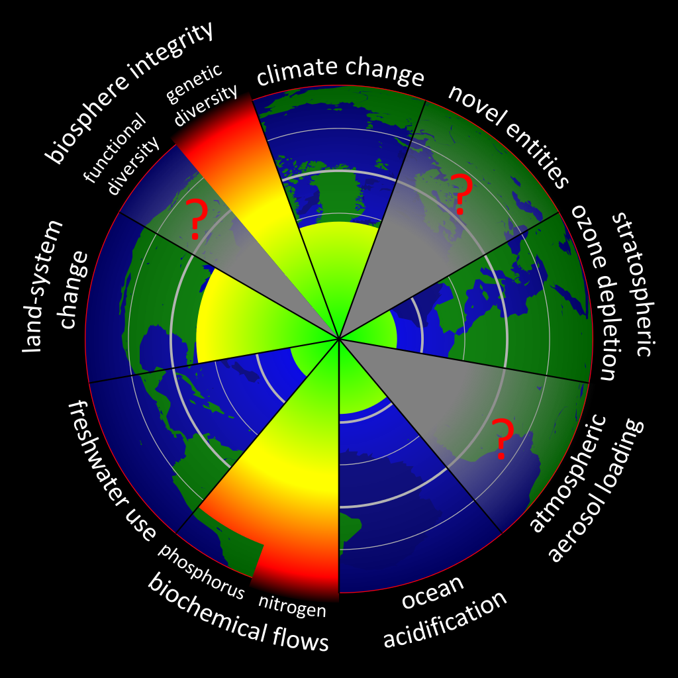
\includegraphics[width=0.6\linewidth]{figures/chap1/planetary_boundaries} 

}

\caption{The planetary boundaries (www.stockholmresilience.org)}\label{fig:f1}
\end{figure}

A more specific example of the plant-environment interactions is the global carbon budget. We are currently facing this significant change in biogeochemical cycling due to the rising fossil fuel emission over the last 150 years. Figure \ref{fig:f2} represents the balance between carbon sources (fossil carbon and land-use changes) and sinks (oceans, land, and atmosphere). The more we emit, the more the Earth system is capturing. Naturally, the emitted CO2 must go somewhere. Approximately half of it is taken up by the ocean and the land (soil + vegetation) sink. As stated earlier, roughly 25\% of the emitted CO2 is dissolved in the ocean sink. The land sink is highly variable: land and soils are very heterogeneous and difficult to model. Nevertheless, the land sink has taken up more emissions in the past 60 years than it did before. The atmosphere is responsible for most of the uptake. This takes us to a question, frequently addressed by global vegetation models, about how long these sinks will continue or not capture our increasing carbon emissions. Note that there is an imbalance: there was more CO2 emitted then absorbed. So, where did the surplus go? This is an active area of research.

\begin{figure}

{\centering 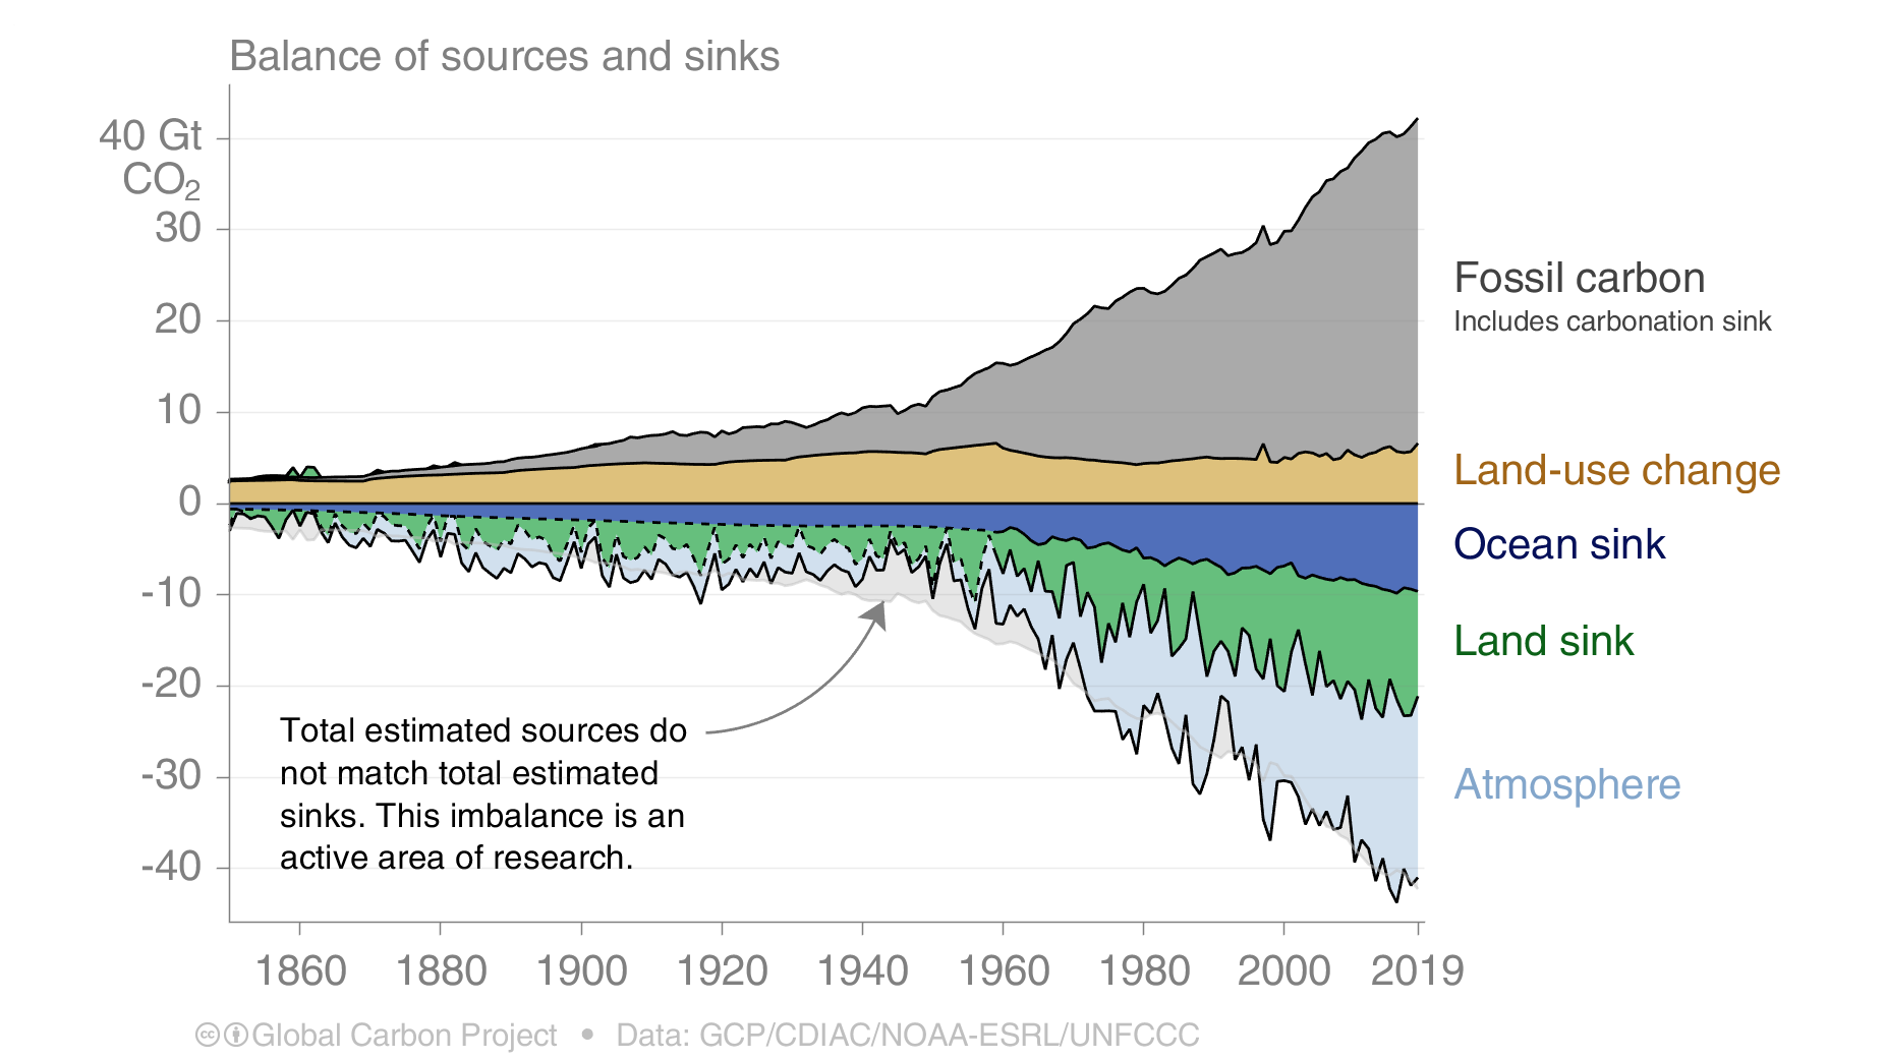
\includegraphics[width=0.8\linewidth]{figures/chap1/carbon_budget} 

}

\caption{The global carbon budget (www.globalcarbonproject.org)}\label{fig:f2}
\end{figure}

\textbf{Climate Models} predict how the long-term weather variation and average weather will evolve. These models include an atmosphere, land and ocean component (Figure \ref{fig:f3} top). The original climate models focused on biophysics: energy and water balances, predicting precipitation, radiation and fluxes between the three components.
More recently, climate models have evolved into \textbf{Earth System Models} (ESM). ESM have a more complex concept because they represents more processes (Figure \ref{fig:f3} bottom). Why? If you want to predict the end of the century climate, we need to consider greenhouse gases and thus the full carbon cycle. ESM are more complex but also more realistic.

\begin{figure}

{\centering 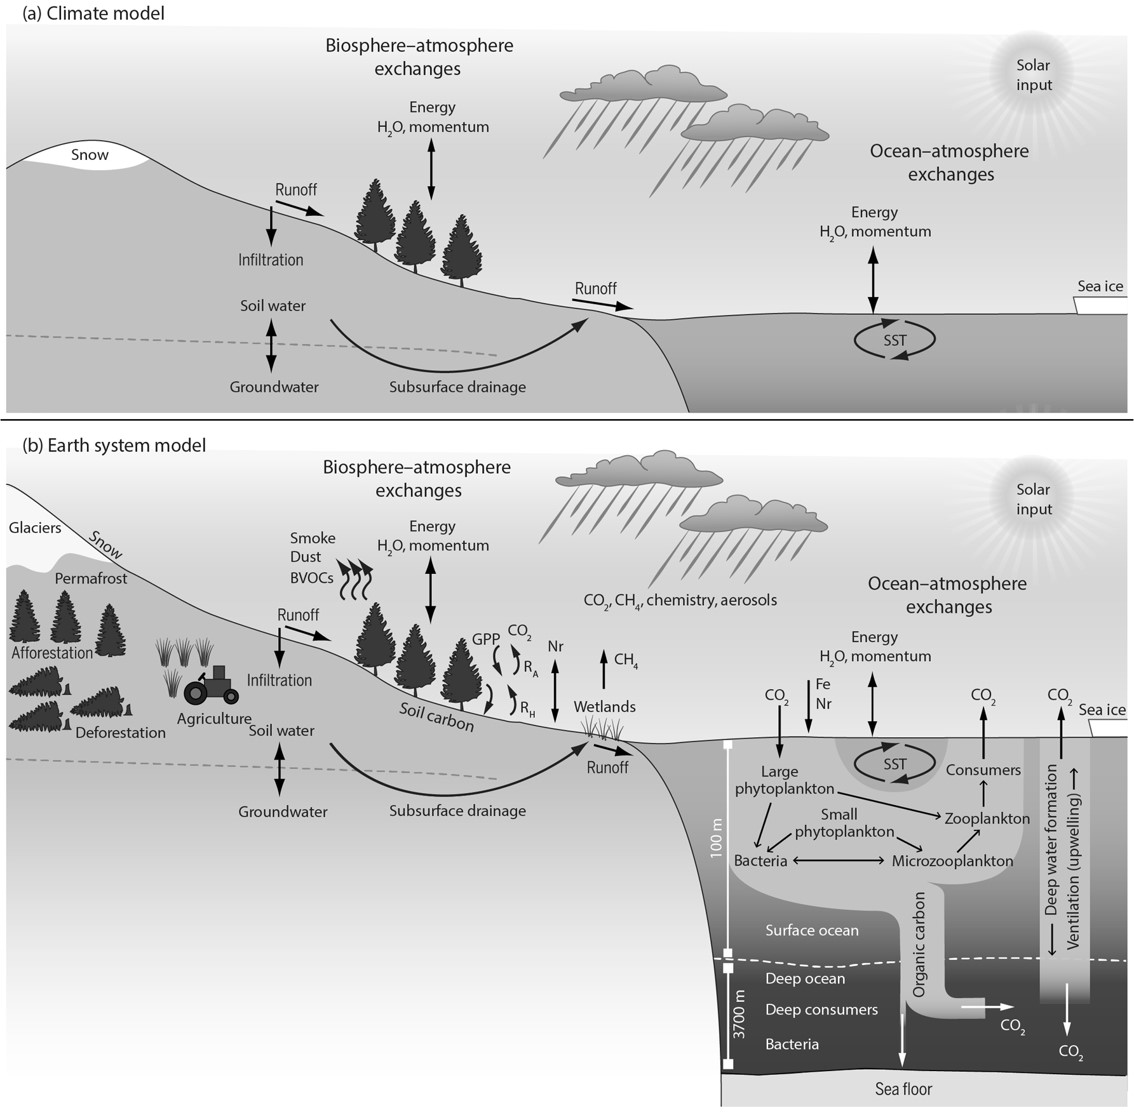
\includegraphics[width=0.7\linewidth]{figures/chap1/GCM_ESM} 

}

\caption{Scientific scope of (a) climate models and (b) earth system models. (Bonan 2019)}\label{fig:f3}
\end{figure}

Vegetation models are often the land component of an earth system model. These `terrestrial biosphere models'(TBM) or `land surface models' (LSM)

\begin{itemize}
\tightlist
\item
  simulate \textbf{energy fluxes}: radiation, evapotranspiration and sensible heat fluxes between the land and the atmosphere. Depending on the vegetation type, the impacts are different.
\item
  simulate the \textbf{hydrology} and the \textbf{carbon cycle}.
\item
  simulate slower processes like \textbf{vegetation dynamics}: the succession of forest or \textbf{land use} and \textbf{urbanization}.
\end{itemize}

\begin{figure}

{\centering 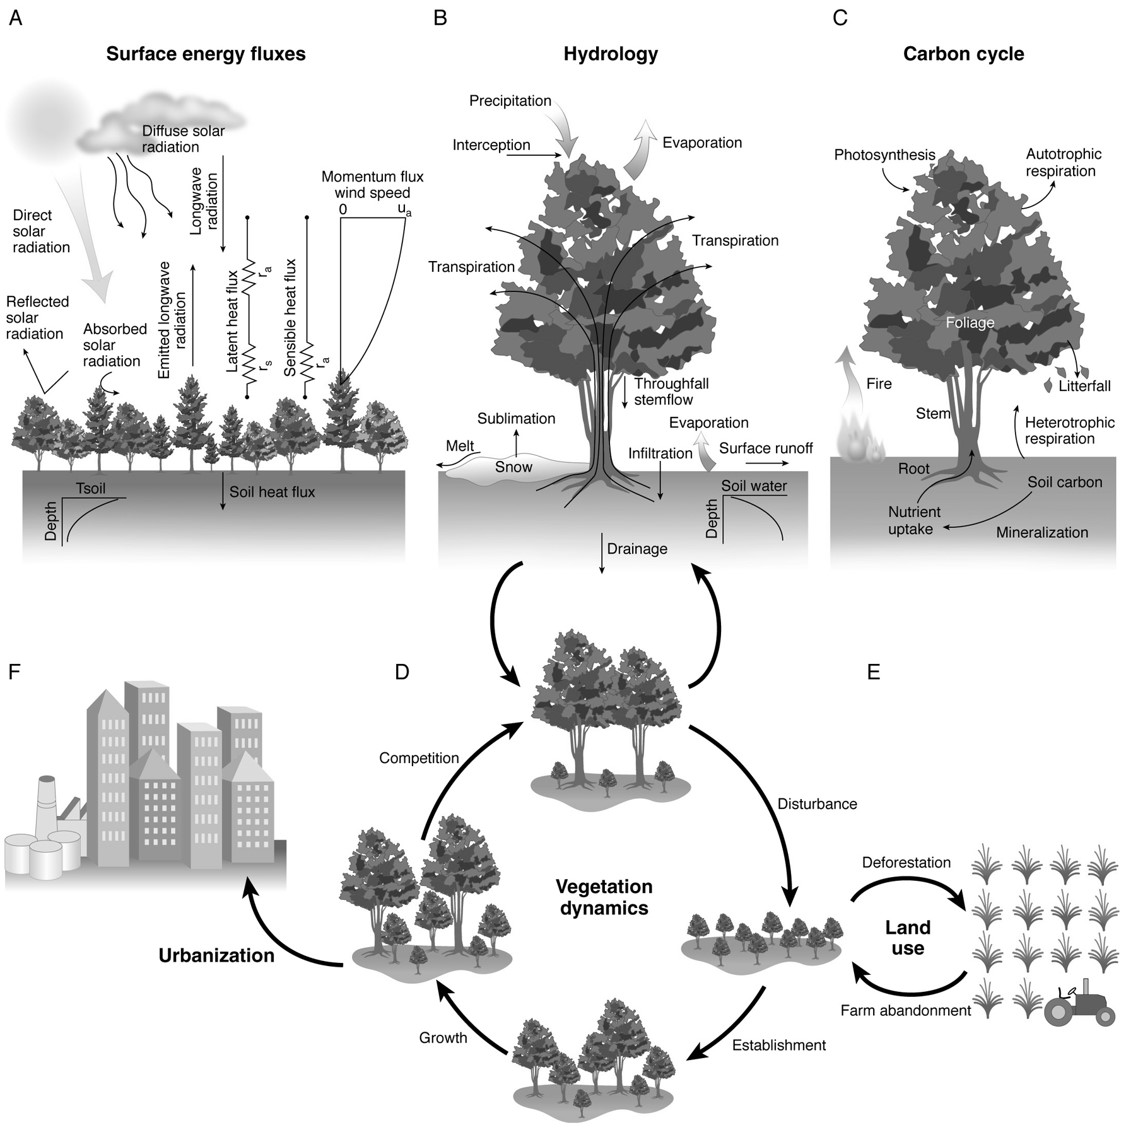
\includegraphics[width=0.8\linewidth]{figures/chap1/cycles_bonan} 

}

\caption{Scientific scope of terrestrial biosphere model. (Bonan 2019)}\label{fig:f4}
\end{figure}

The coupler is a system that links different models. For example the terrestrial biosphere can be seen as the coupler between geochemistry and hydrology. A coupler can be the link between more than two other systems, so that a kind of satellite system is formed. The land model is mostly seen as the coupler. This results in the fact that both fast and slow processes depend on each other. The surface energy flux is an example of a fast process since it varies over the course of one day Vegetation dynamics on the other hand, is a slow process. Succession does not happen overnight.

\hypertarget{why-do-we-need-modelling}{%
\section{Why do we need modelling?}\label{why-do-we-need-modelling}}

Modelling has proven to be a essential tool:

\begin{itemize}
\tightlist
\item
  For \textbf{understanding}: we need good theoretical foundations (understand processes) to generalize knowledge and observations in space and time (upscaling). Studying the inaccuraies in models leads to the formulation of new hypotheses.
\item
  For \textbf{prediction}, how vegetation responds to expected changes (temperature or CO2) to develop management strategies and policies.
\item
  For \textbf{data integration}: a framework to bring together multiple data sources and to guide future data collection.
\end{itemize}

\hypertarget{model-types}{%
\section{Model types}\label{model-types}}

How can we look at the different model types that exist (Table \ref{table:example})? Models are to be placed in a continuum ranging from empirical to process-based models. \textbf{Empirical models} are based on data and correlations, not describing precisely the biophysical processes --- \textbf{process-based models} describing the biophysical processes and causal relations between the variables (Table \ref{table:empiricial}). Most existing vegetation models are hybrid.

\begin{center}
\captionof{table}{Continuum of terrestrial biosphere/ecosystem models. (Bonan 2019)}
\label{table:example}

\begin{center}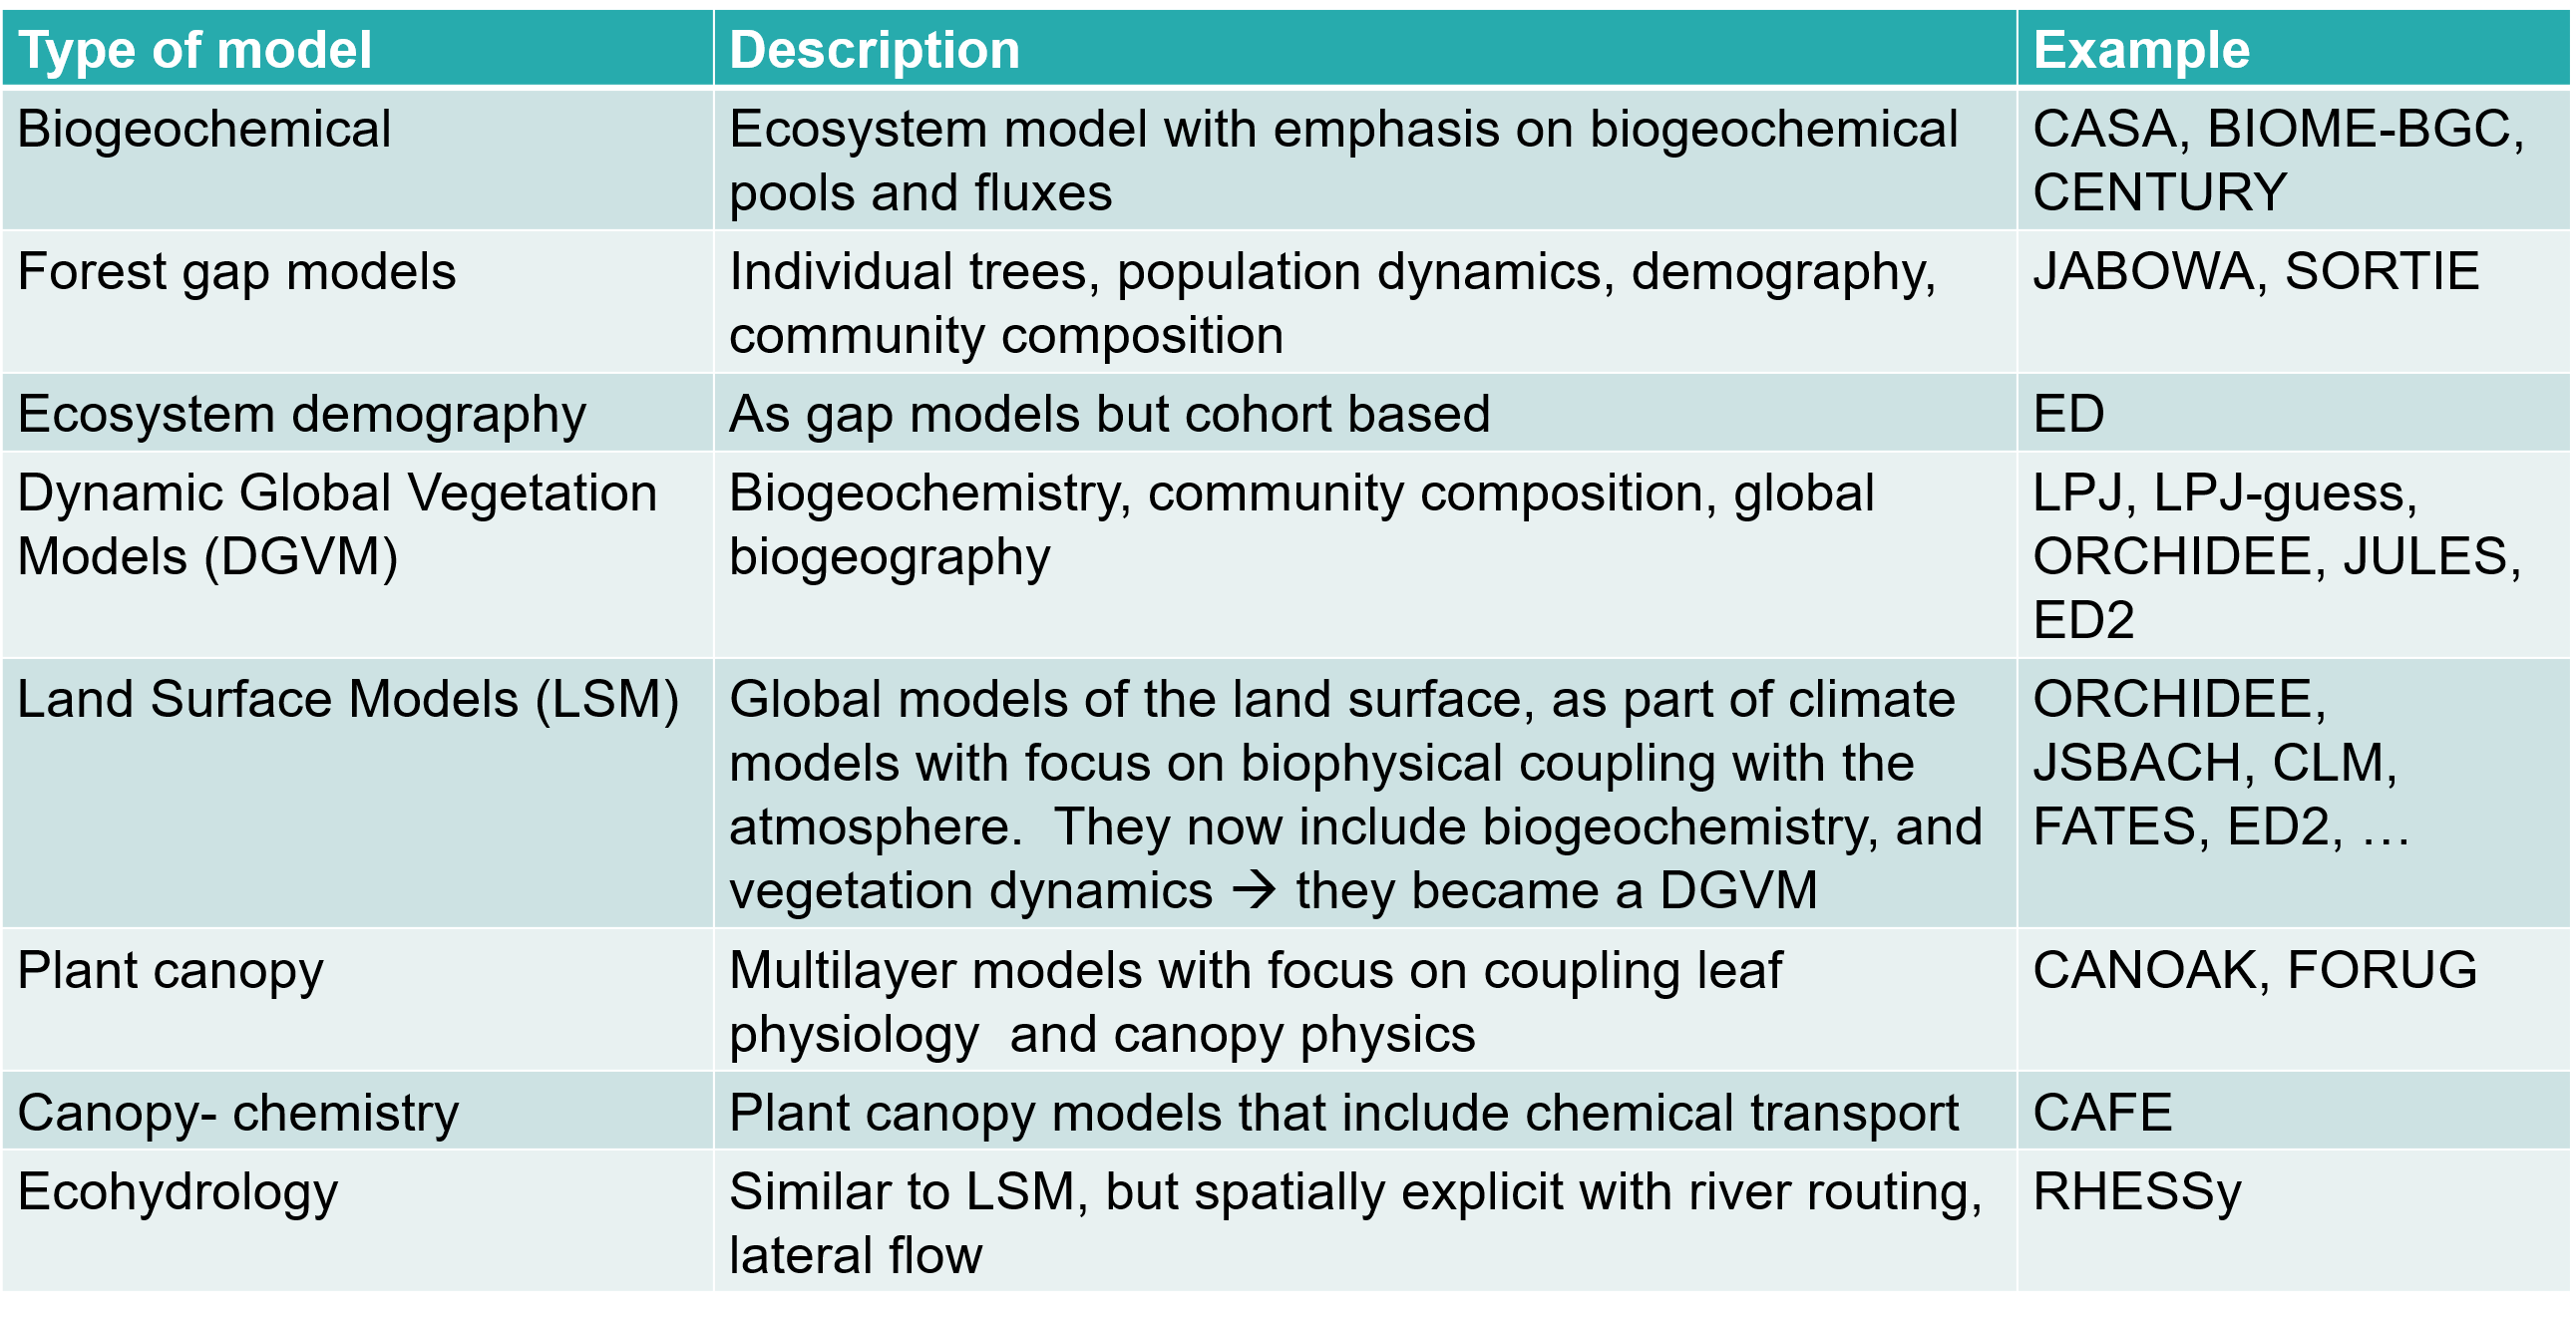
\includegraphics[width=0.8\linewidth]{figures/chap1/table_model_types} \end{center}
\end{center}

\begin{center}
\captionof{table}{Continuum of process-based versus empirical models. (Adams et al. 2013)}
\label{table:empiricial}

\begin{center}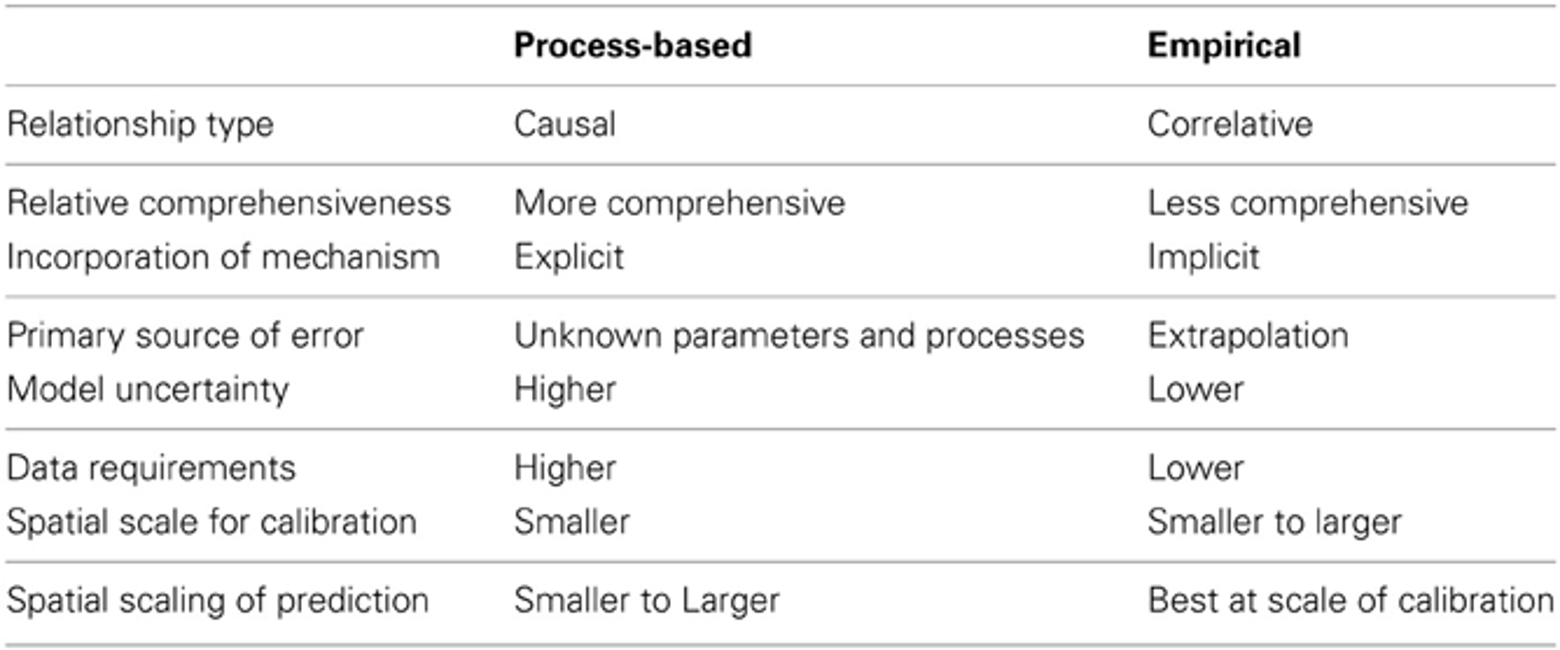
\includegraphics[width=0.8\linewidth]{figures/chap1/tables_PB_empirical} \end{center}
\end{center}

The model type depends on:
- Purpose: will it be used for management support, policy support, research.
- Question: different people will be interested in different questions (foresters, ecologists, policy makers\ldots)
- Scale: models that are to be applied for local use can be much more detailed than worldwide models because data gathering is much more straightforward on a small scale. Also the time-scale is of importance: will the model be used for research about the past, the present or the future?

\hypertarget{the-history-of-vegetation-models}{%
\section{The history of vegetation models}\label{the-history-of-vegetation-models}}

The history of vegetation models is one that parallels that of the computer. Computers made it possible to calculate much faster and much more, which made them suitable for modelling. The first vegetation models have emerged in the 1960s and 1970s.

One of the first models were the \textbf{box models} (1960); these models describe the flow of mass and energy through boxes. These models still exist in current biogeochemical models, where arrows represent the fluxes between the pools. In parallel, \textbf{gap models} had emerged. Gap models simulate the dynamics of the development of a gap in a forest and the growth of plants in this gap. Gaps can be created by fallen trees, by dead trees, \ldots{} . This kind of models are individual-based and focused on population dynamics and the life cycle of species: growth, regeneration and mortality while taking environmental constraints in account. These models are the first models that were ever used for upscaling: from tree level, to plot-level, to landscape level. They were developed by forest scientists using forest inventories to derive growth, regeneration, and mortality in response to environmental variables.
In 1973, the first model (MIAMI model by Lieth (1973)) was developed to derive global net primary productivity (NPP), relating NPP in an empirical way to climate variables (temperature) with vegetation productivity. This was the first attempt to make a global upscaling of a vegetation process.
In the 1980s surged the first \textbf{land surface models}. Land surface models are the models where the other models start to integrate into, and evolved as such into -- \textbf{Terrestrial biosphere models} (see Figure \ref{fig:f7}), which are now the state-of-the-art land components of ESMs.
Vegetation modelling therefore is a very interdisciplinary field because it involves knowledge of different scientific fields, making it difficult to find a common terminology. Global EMS are currently still not good to simulate realistic vegetation dynamics.

\begin{figure}

{\centering 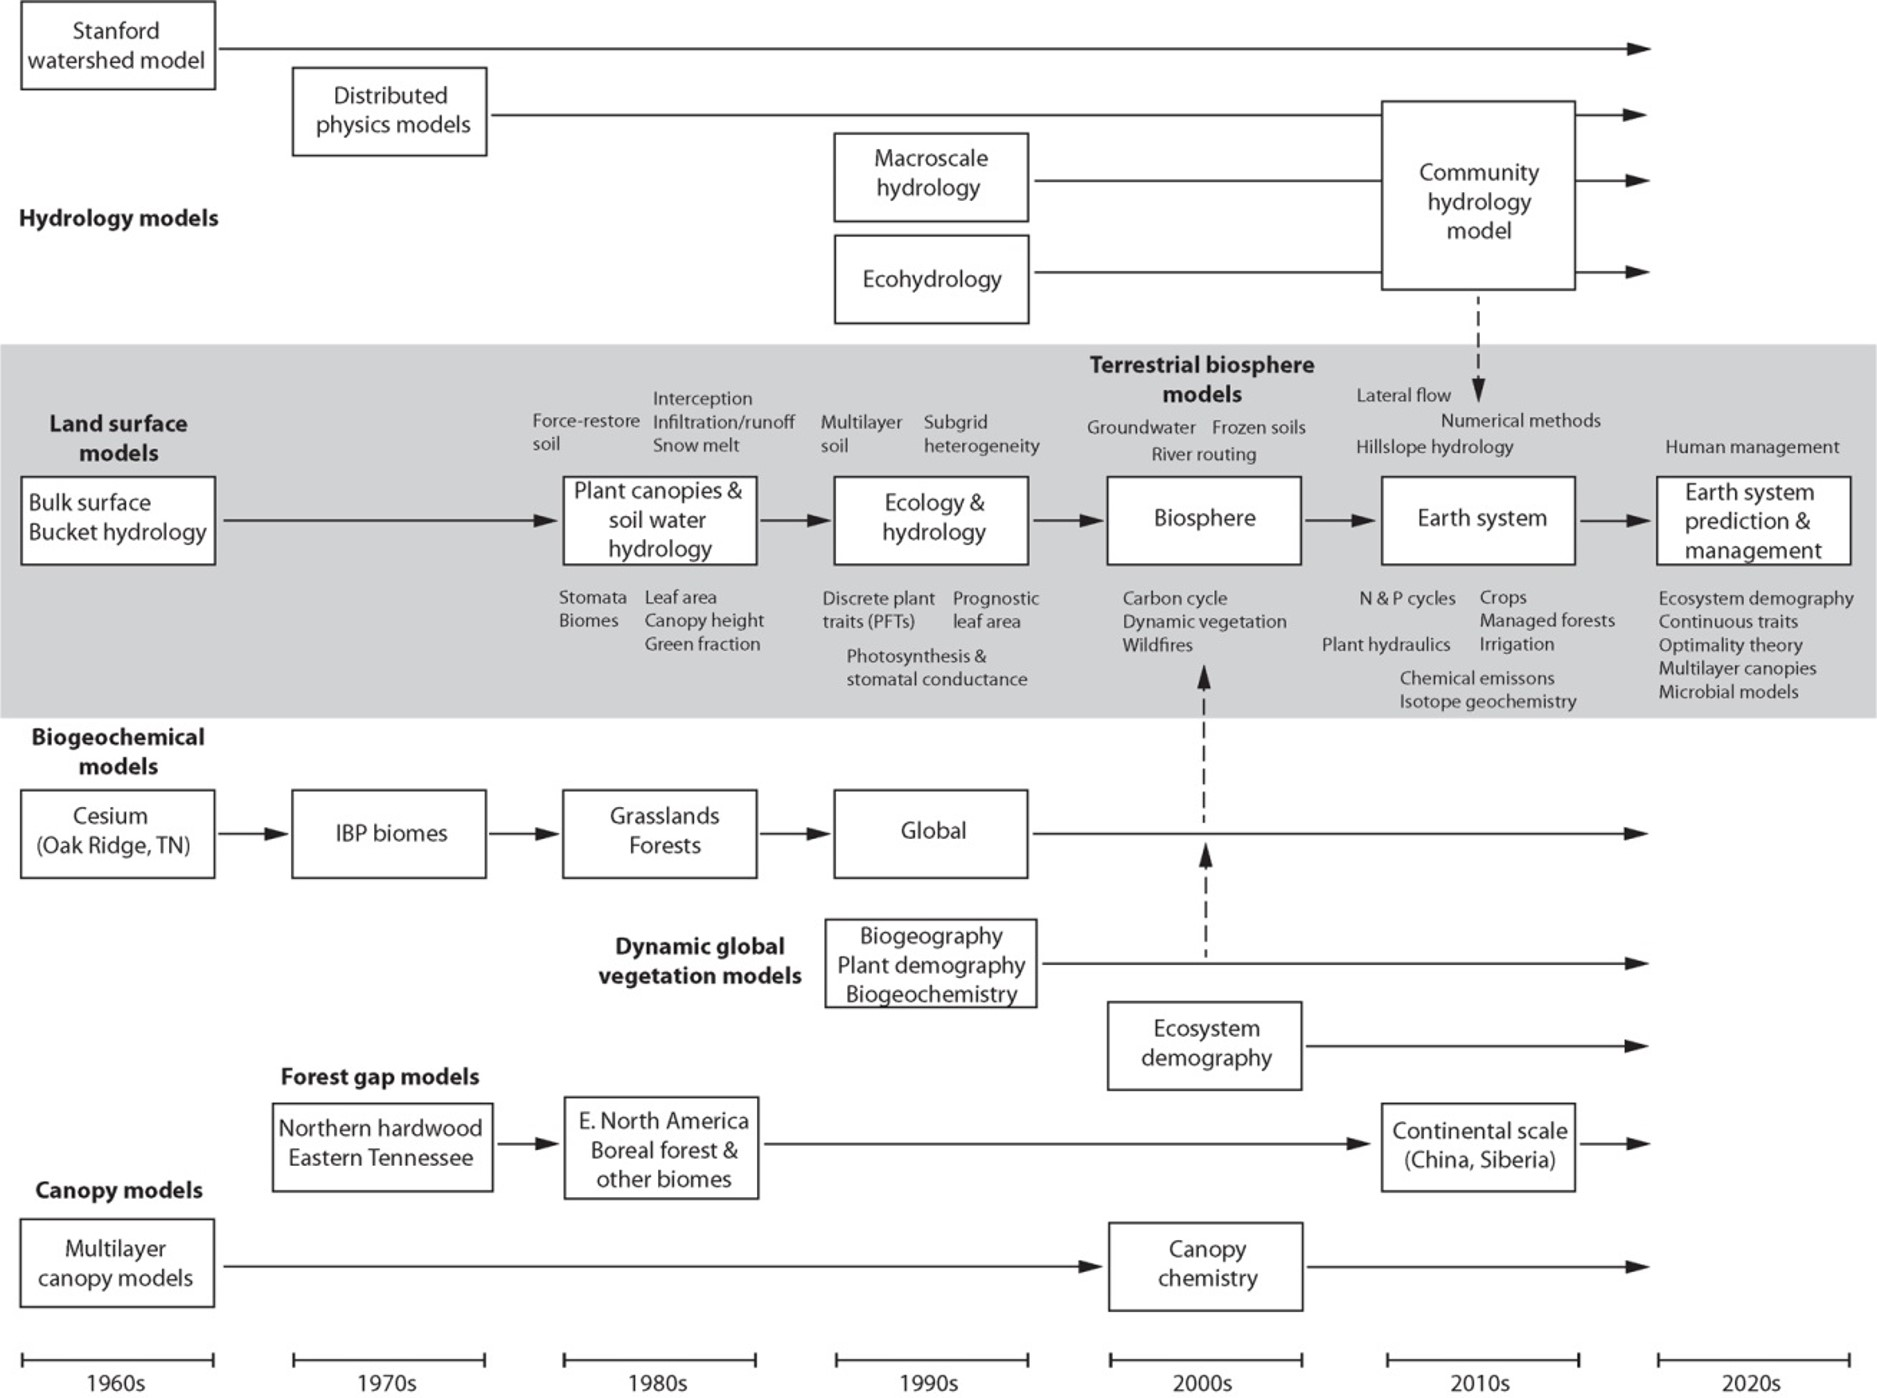
\includegraphics[width=0.8\linewidth]{figures/chap1/timeline} 

}

\caption{Timeline showing the parallel development of model types and the integration of model types into land surface models towards terrestrial biosphere models. (Bonan 2019)}\label{fig:f7}
\end{figure}

\hypertarget{components-of-a-model}{%
\section{Components of a model}\label{components-of-a-model}}

What is a vegetation model?
Two attempts for a definition:

\begin{itemize}
\tightlist
\item
  \textbf{Dynamic global vegetation models} (DGVMs) are powerful tools to project past, current and future vegetation patterns and associated biogeochemical cycles (Scheiter et al., 2013).
\item
  A \textbf{Dynamic Global Vegetation Model} (DGVM) is a computer program that simulates shifts in potential vegetation and its associated biogeochemical and hydrological cycles as a response to shifts in climate. DGVMs use time series of climate data and, given constraints of latitude, topography, and soil characteristics, simulate monthly or daily dynamics of ecosystem processes. DGVMs are used most often to simulate the effects of future climate change on natural vegetation and its carbon and water cycles (Wikipedia 2021).
\end{itemize}

\begin{center}
\captionof{table}{Definition of key model components and examples for a typical TBM}
\label{table:components}

\begin{center}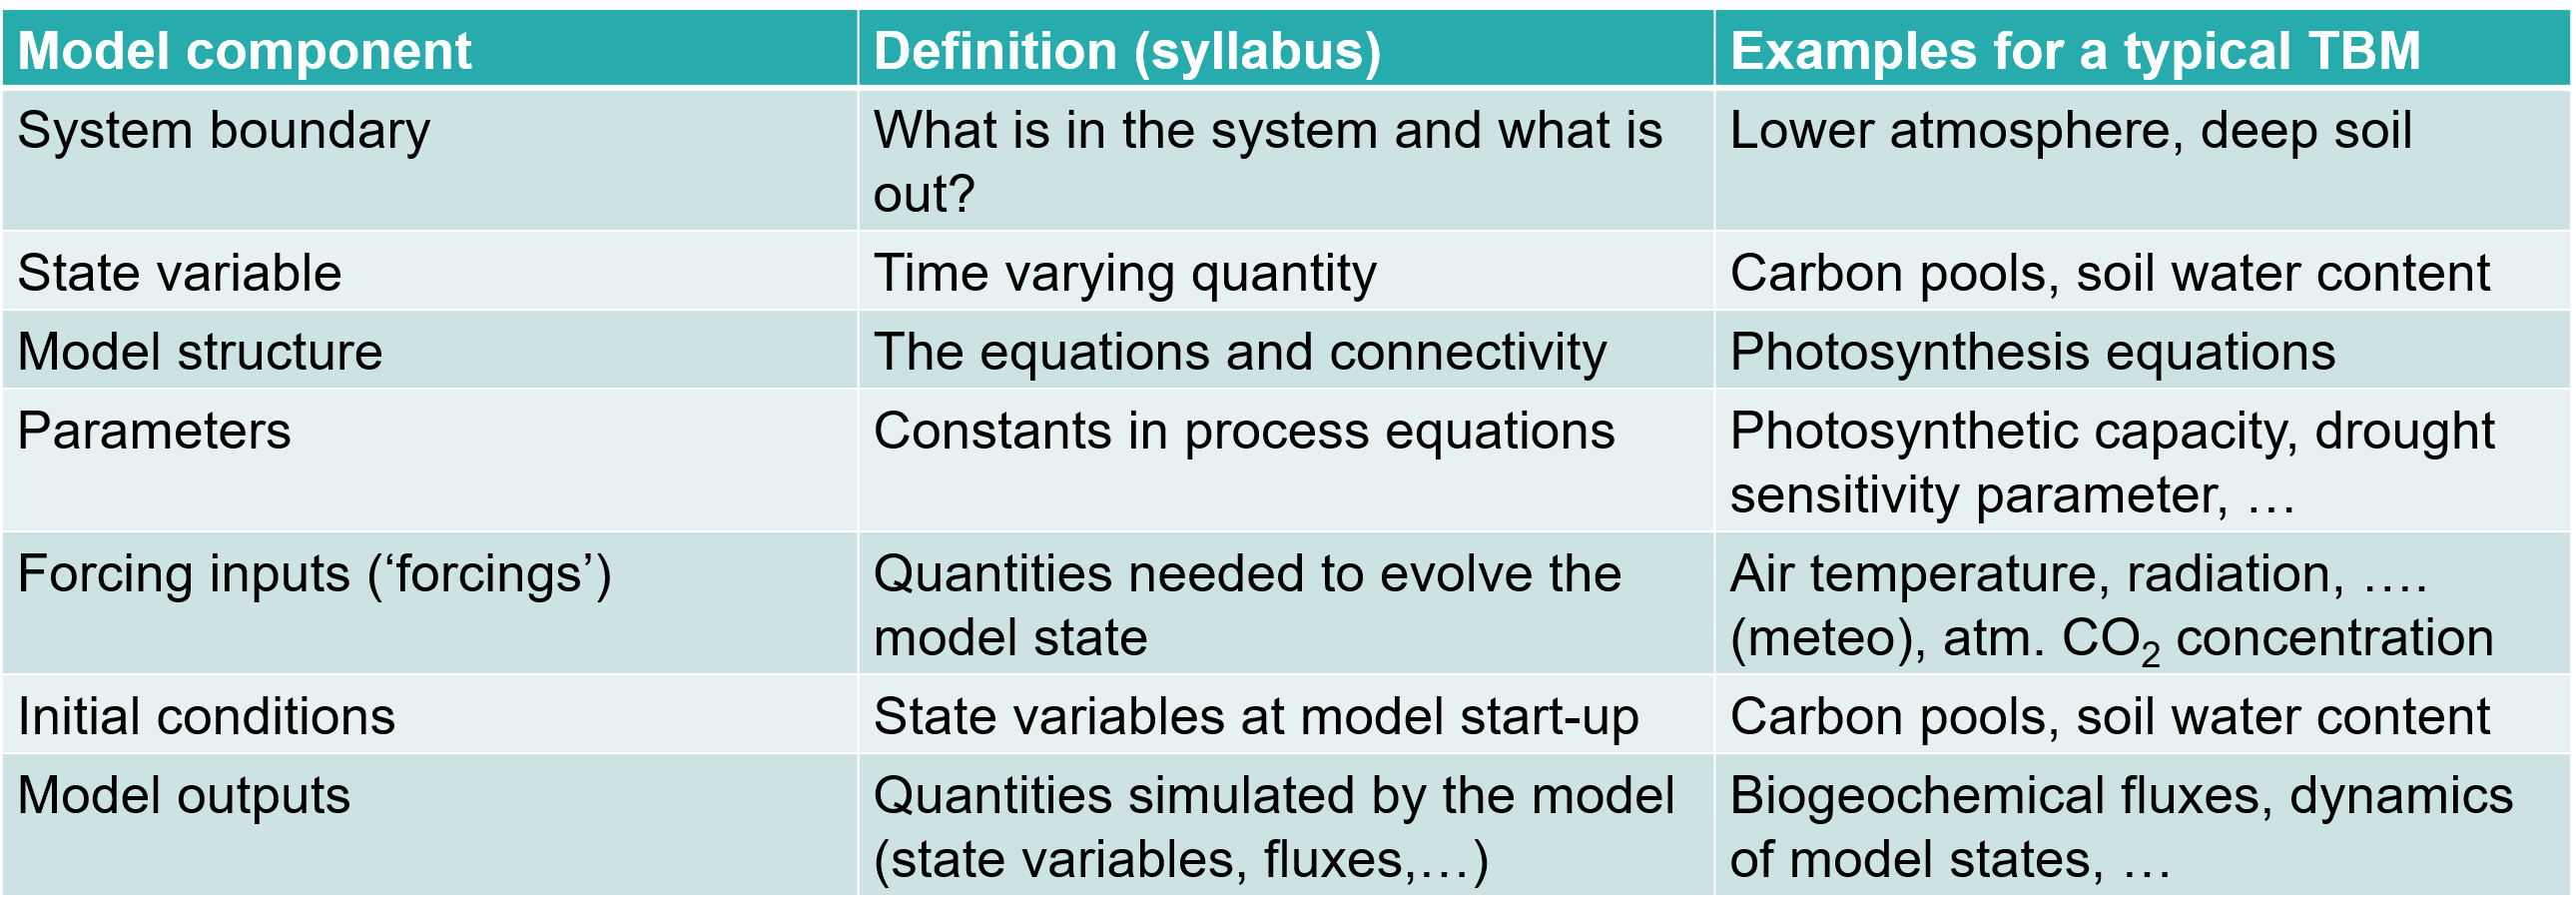
\includegraphics[width=0.9\linewidth]{figures/chap1/table_components} \end{center}
\end{center}

\hypertarget{processes}{%
\subsection{Processes}\label{processes}}

They are a key component because we are focusing on process-based models in this course. There is a long list of processes (energy, water, turbulent transport, canopy scaling, carbon, nitrogen, trace gasses, demography,\ldots) that the models integrate, especially the more complex ones. These processes will be discussed in detail in the following theory chapters and we will mainly focus on how to translate them into equations.

\hypertarget{equations}{%
\subsection{Equations}\label{equations}}

These are the mathematical representations of the processes. However, there are important constraints to insert equations into a vegetation model, such as the specific time scale at which a process operates. For example, it makes little sense to resolve the equation for forest composition (succession) on a daily calculation time step. This is a prolonged process with an extremely low variance between consecutive days. The solution for the equation for photosynthesis, on the other hand, varies significantly throughout the day and between consecutive days (cloudy day vs sunny day).

There are three types of equations within vegetation models:
- \textbf{prognostic equations}: time derivatives of differential equations -- they calculate the state's change over time
- \textbf{conservation equations}: equations describing the conservation of mass and energy
- \textbf{diagnostic equations}: linking multiple variables independent from the time.

Often there is no analytical solution of the equations describing on-linear processes in biological systems; therefore, we must use numerical methods to solve the equations.

\hypertarget{parameters}{%
\subsection{Parameters}\label{parameters}}

These are the constants in the model. Some parameters are highly uncertain because we cannot measure them very well at the relevant scale. For example, we can make reliable measurements of the photosynthetic capacity of a single leaf. However, upscaling this parameter so that it is applicable for a forest or multiple PFTs (= plant functional types) induces uncertainty. The more parameters a model uses, the more uncertainties that are to be taken into account.

\hypertarget{time-steps}{%
\subsection{Time Steps}\label{time-steps}}

Vegetation models run at multiple timescales (combining processes that are resolved at multiple timescales). Models present fast processes, which are calculated every hour (e.g.~photosynthesis and energy balance), intermediate processes calculated daily (e.g.~carbon allocation and growth) and slow processes in order of years (e.g.~mortality) (Fig.6).

\begin{figure}

{\centering 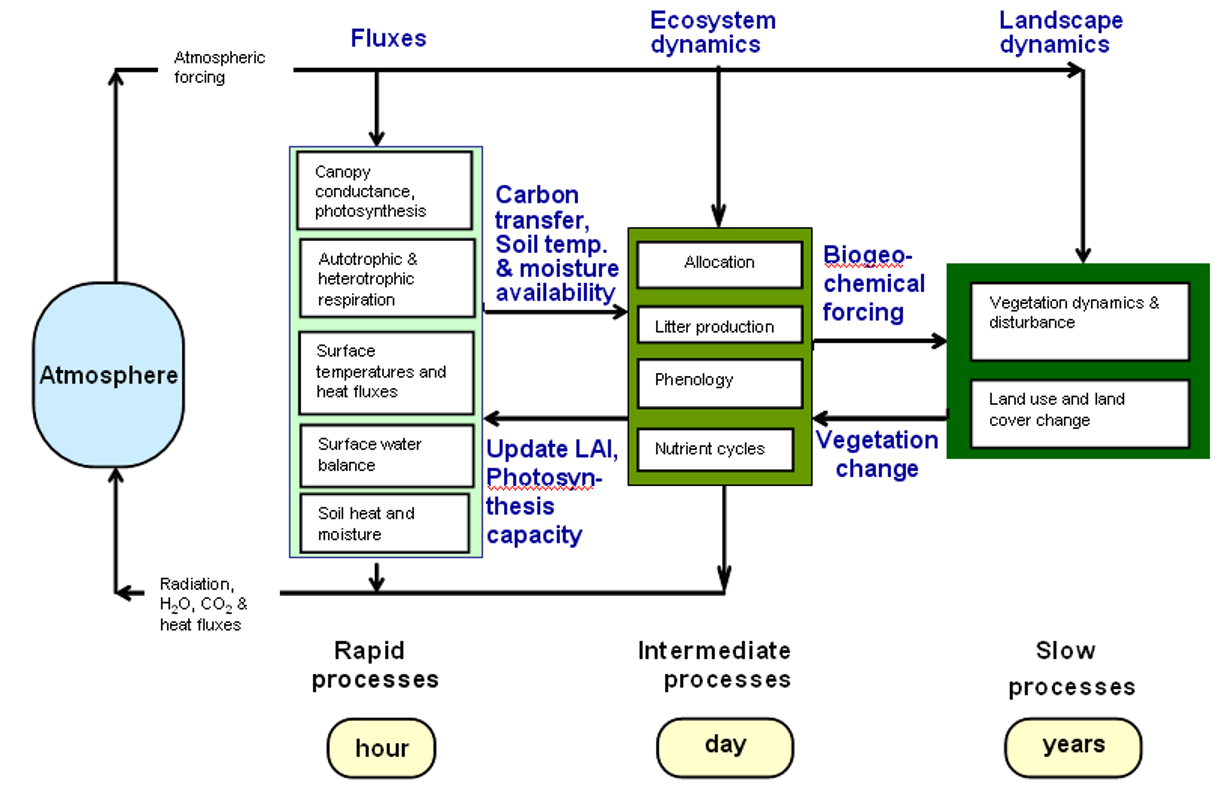
\includegraphics[width=0.8\linewidth]{figures/chap1/time_steps} 

}

\caption{Structure of a vegatation model indicating the different time steps at which each process is simulated (Williams et al. 2009)}\label{fig:f9}
\end{figure}

\hypertarget{spatial-structure}{%
\subsection{Spatial structure}\label{spatial-structure}}

The division of space in voxels, layers or grid cells and its resolution determines how many times we repeat our calculations in space. Global vegetation models have a typical spatial grid of 100km or even more and divide the landscape into patches. In each patch, they simulate the vegetation (forest, savannas, grassland\ldots). Models also have a horizontal grid or horizontal layering: some models consider multiple soil layers. The same is true for above ground layers, where some models divide the canopy into multiple layers (Figure \ref{fig:f10}).
For example, the Ecosystem Demography Model (ED2.2) divides the forest into multiple grid cells where the same meteorological conditions apply within each grid cell. Then within each cell, this model has different sites with different soils. Each site is divided into multiple patches (forests with a similar disturbance history). For each patch, the model simulates multiple cohorts of trees where size and plant functional types play a role (Figure \ref{fig:f11}).

\begin{figure}

{\centering 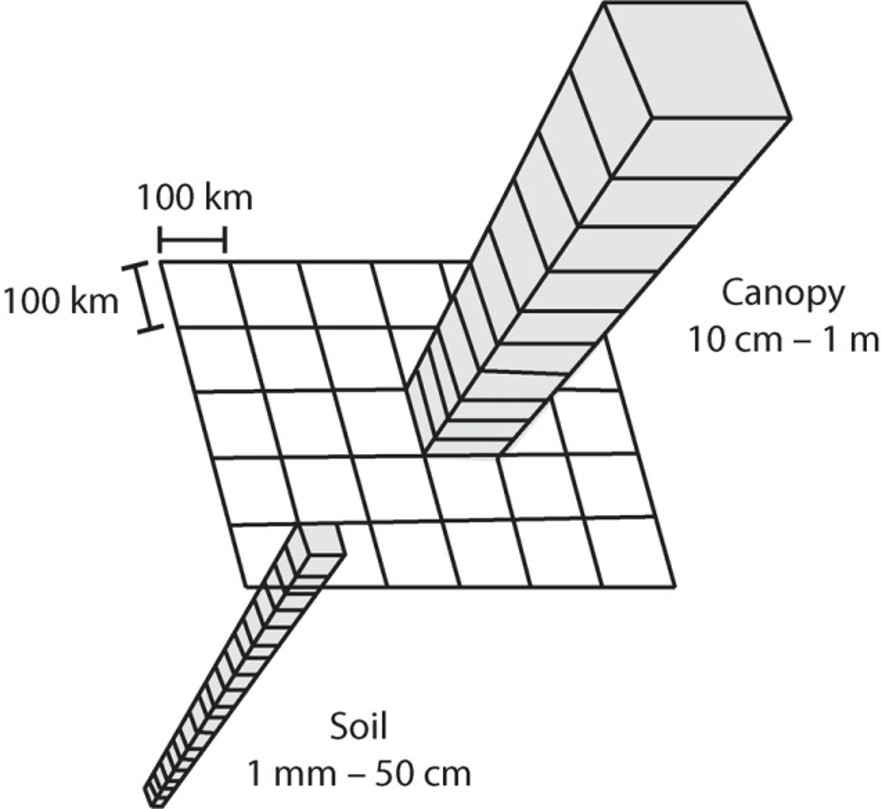
\includegraphics[width=0.5\linewidth]{figures/chap1/grid_vert_hor} 

}

\caption{Three dimensional grid of a TBM structured in terms of longitude x latitude x level. The number of soil and canopy layers and the geographical resolution is model dependent, (Bonan 2019)}\label{fig:f10}
\end{figure}

\begin{figure}

{\centering 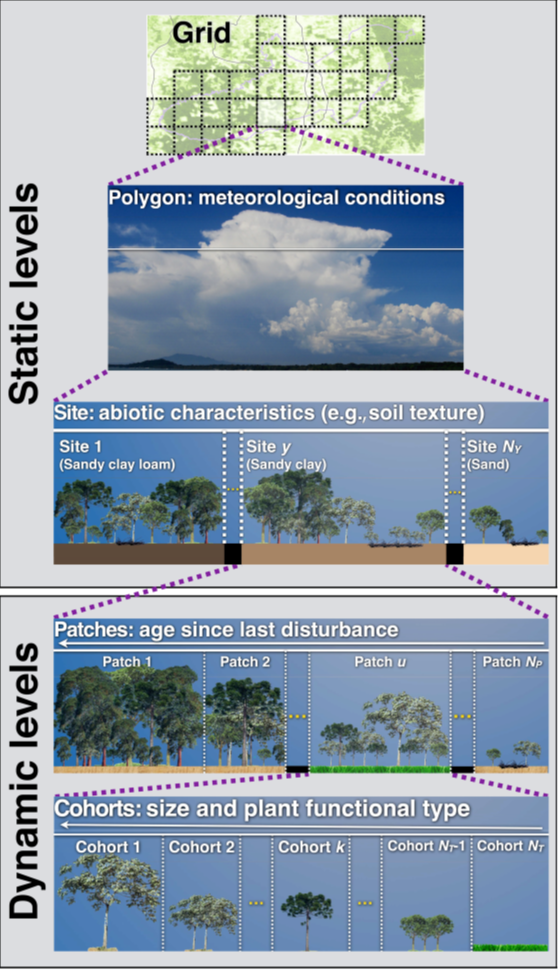
\includegraphics[width=0.7\linewidth]{figures/chap1/grid_ED2} 

}

\caption{Example: the spatial multi-level grid structure of of the ED2 vegetation model (Longo et al. 2019)}\label{fig:f11}
\end{figure}

\hypertarget{model-code-complexity-and-uncertainty}{%
\subsection{Model code, complexity and uncertainty}\label{model-code-complexity-and-uncertainty}}

There is a gap between equations and how the are implemented in the actual model code. Also, a specific process can be implemented into an equation in various ways. Usually, large models also contain a ``technical debt'', which means over the years, multiple modelers have continued working on models and added code lines, but at some point, the code is so large that none of the developers still knows the entire code, resulting in persistent bugs or overlooked assumptions.

Models are always a simplification of the real world, but they tend to become overly complex.

More complex models (adding more processes) become more realistic, but we also add more sources of uncertainty. Therefore, we should choose our model carefully based on the research question we want to adress.

\hypertarget{data}{%
\subsection{Data}\label{data}}

It is not possible to develop models without data. In general, the more data (multiple data sources), the better.

\hypertarget{modelling-workflow-and-structure-of-the-course}{%
\section{Modelling workflow and structure of the course}\label{modelling-workflow-and-structure-of-the-course}}

Vegetation modelling is a multidisciplinary field. This course will mainly focus on the mathematical formulation of processes and translating these equations into a working model.

\begin{figure}

{\centering 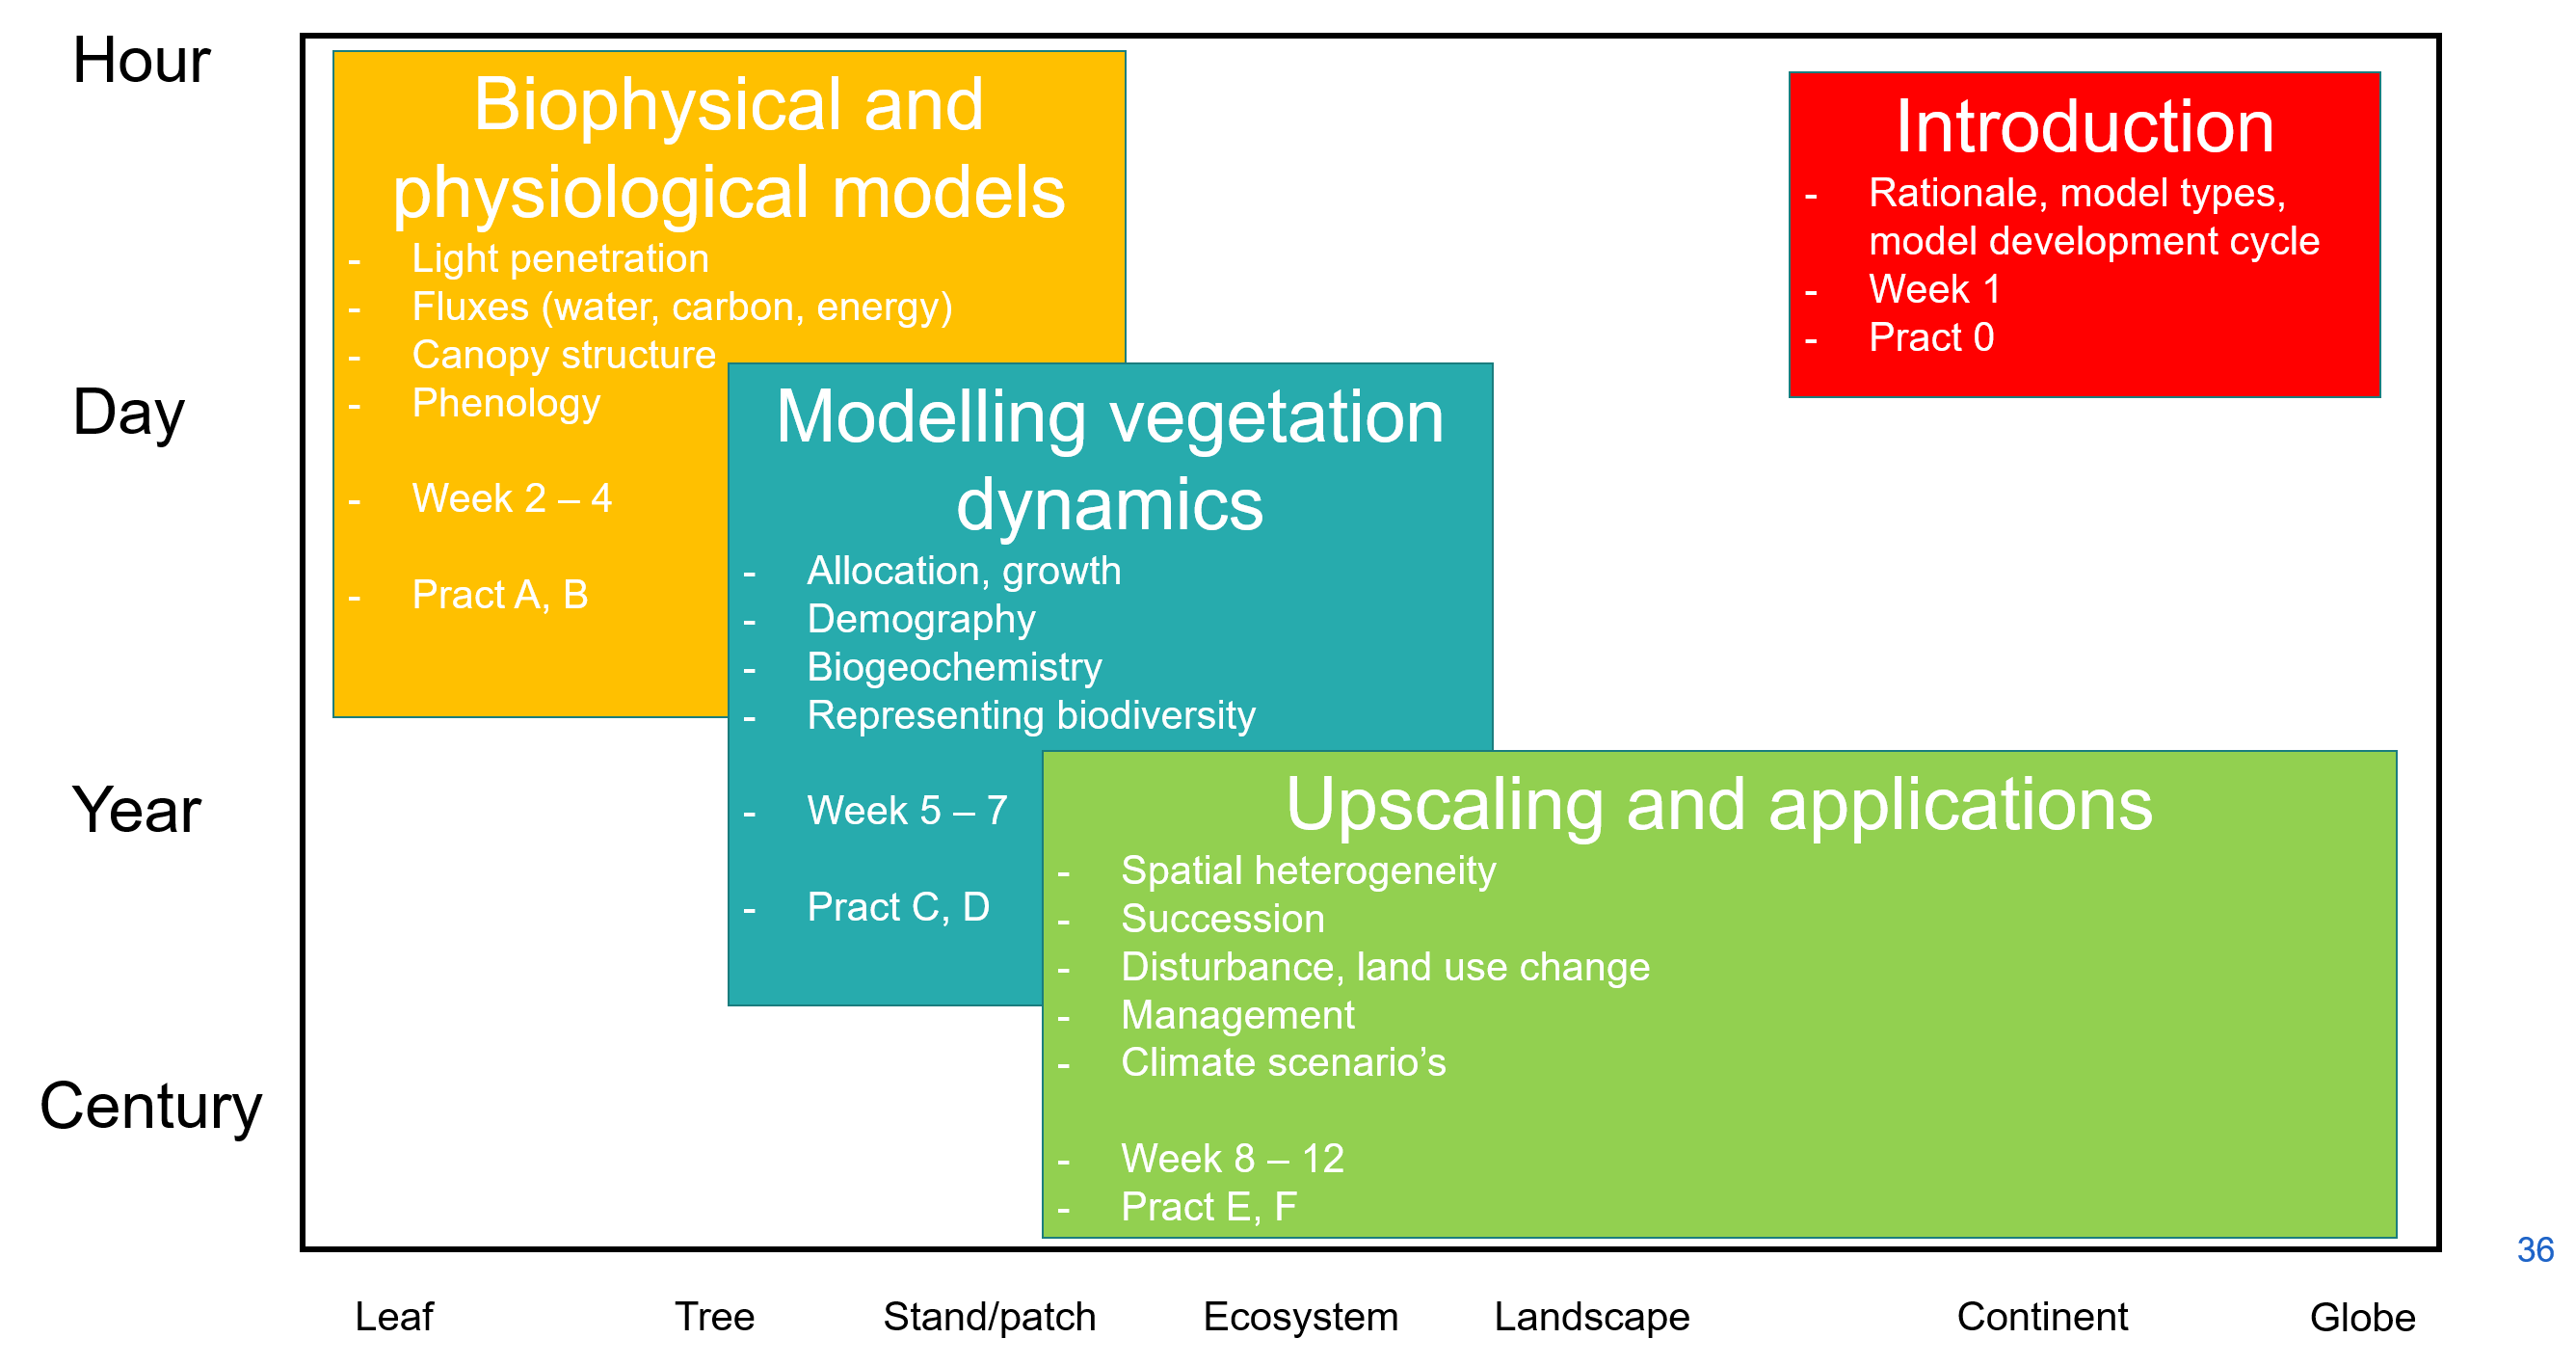
\includegraphics[width=0.9\linewidth]{figures/chap1/course_overview} 

}

\caption{Progression through spatial and temporal scales throughout this course}\label{fig:f12}
\end{figure}

The construction of a model is a continuous process -- a model is never finished. As Figure 10 shows us, we start by describing our system in the form of equations, then running the computer program to characterize the model, perform parameter estimation and interpretation, and then apply it to other locations and validate against independent data.

\begin{figure}

{\centering 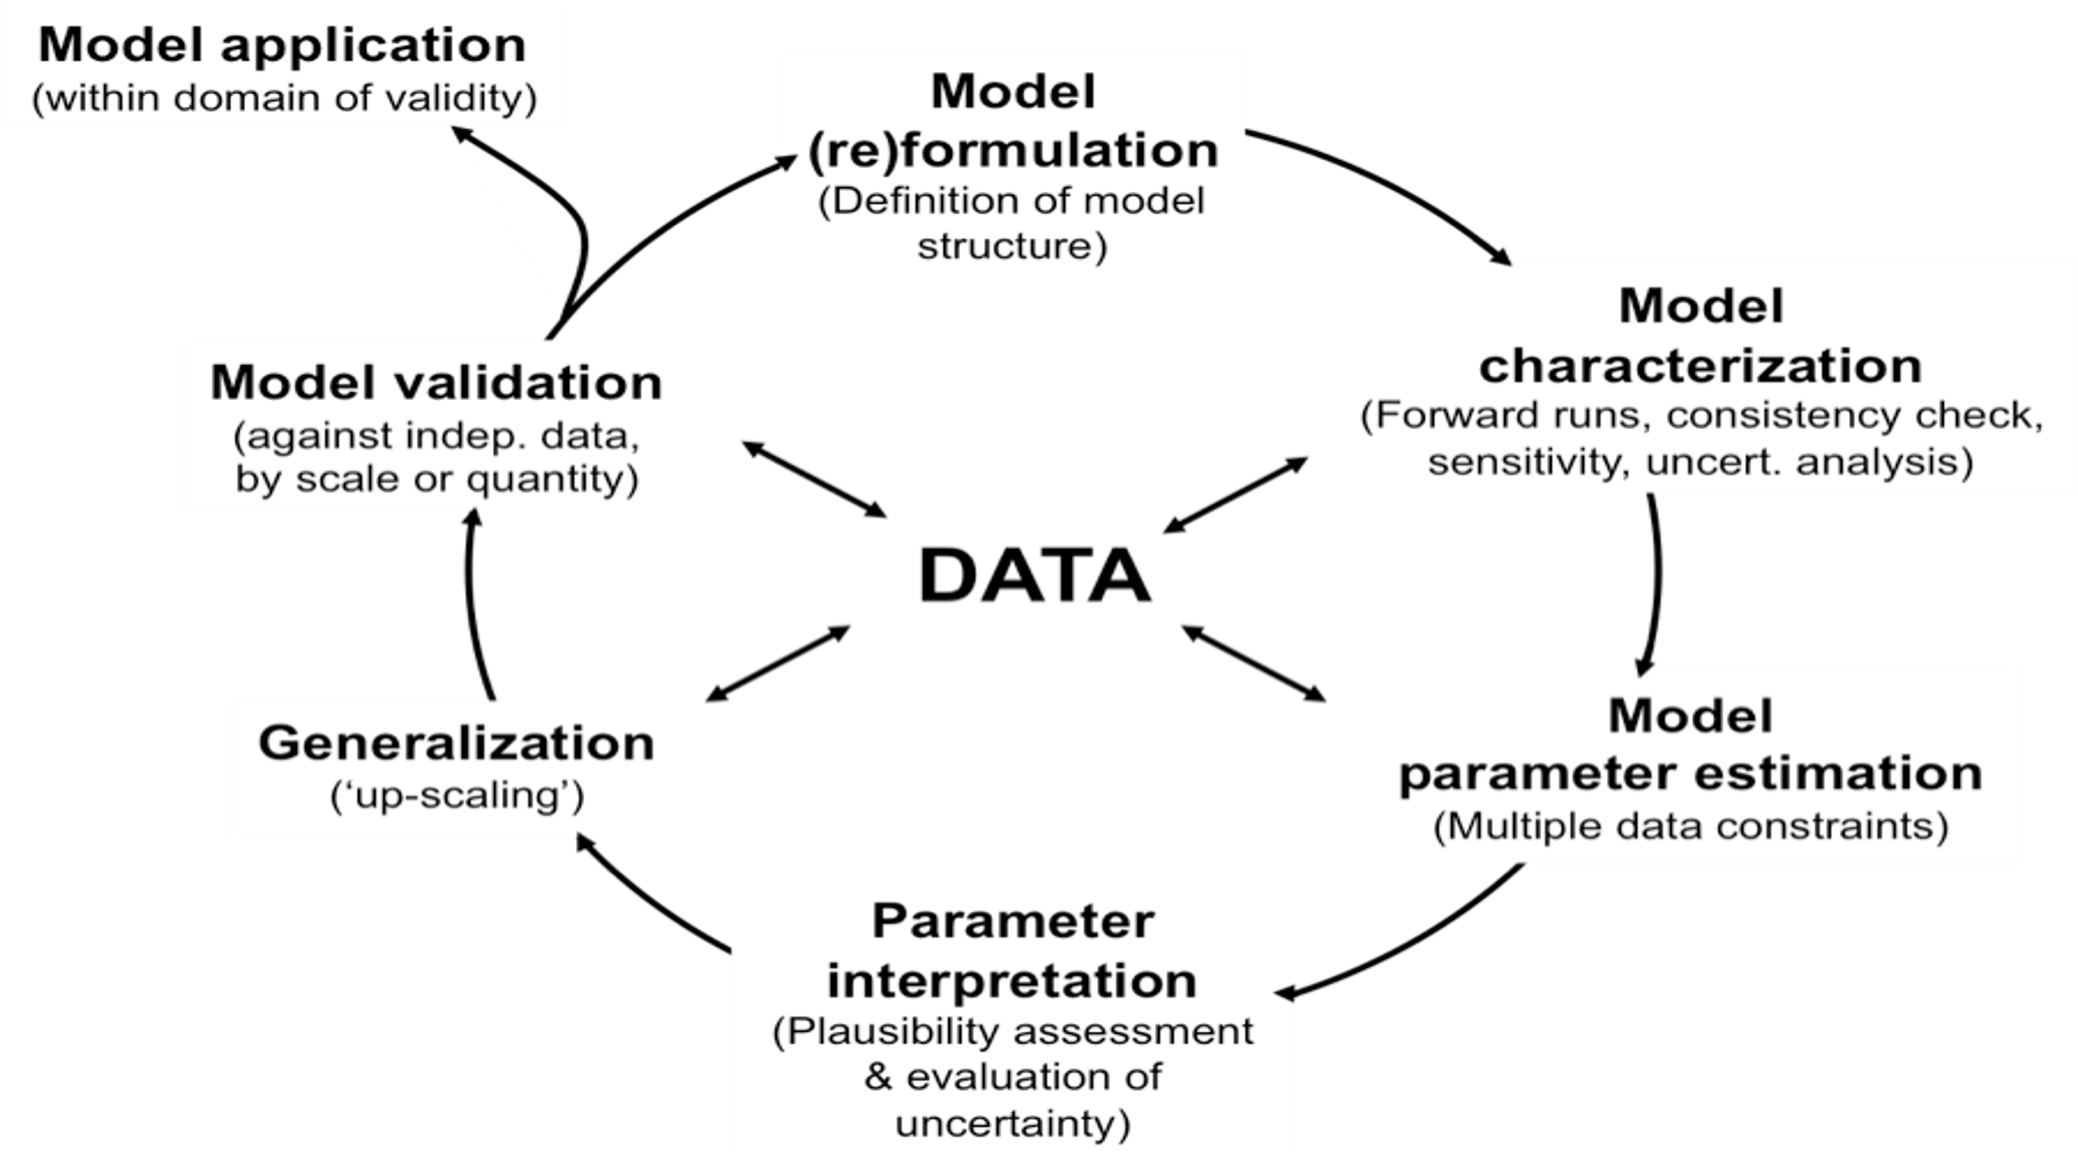
\includegraphics[width=0.8\linewidth]{figures/chap1/williams_fusion} 

}

\caption{Model data fusion in every step of the model development cycle (Williams et al. 2009)}\label{fig:f13}
\end{figure}

\begin{figure}

{\centering 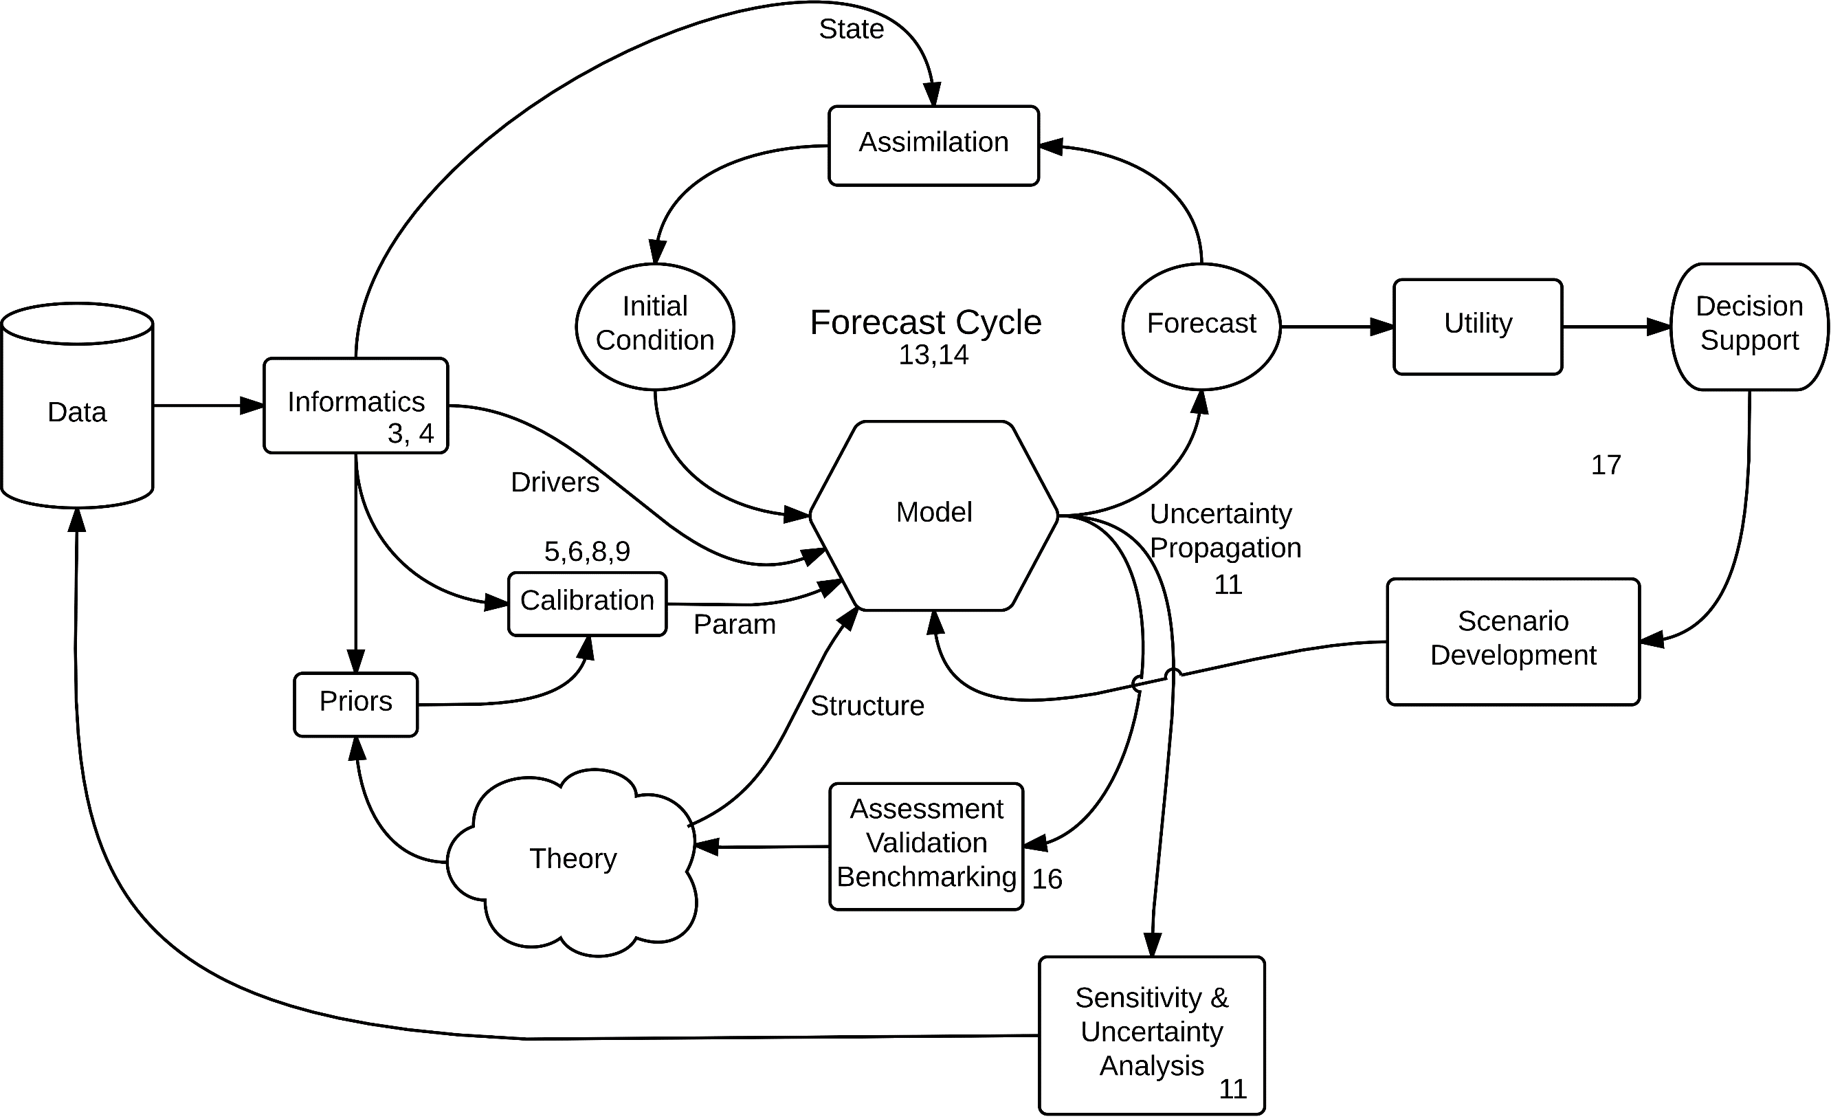
\includegraphics[width=0.8\linewidth]{figures/chap1/dietze_workflow} 

}

\caption{Methodological workflow of model data fusion (Dietze: Ecological Forecasting)}\label{fig:f14}
\end{figure}

\hypertarget{part-biophysical-and-physiological-models}{%
\part{Biophysical and physiological models}\label{part-biophysical-and-physiological-models}}

\hypertarget{modelling-plant-basic-processes}{%
\chapter{Modelling plant basic processes}\label{modelling-plant-basic-processes}}

\chaptermark{photsynthesis}

\hypertarget{photosynthesis-models}{%
\section{Photosynthesis models}\label{photosynthesis-models}}

Photosynthesis is a process that takes place in all plants on earth. There is a huge variability in photosynthesis rates in space and time because of environmental variations (weather/climate) and properties of the vegetation (species composition, structure).

\hypertarget{refreshing-the-basic-knowledge}{%
\subsection{Refreshing the basic knowledge}\label{refreshing-the-basic-knowledge}}

Leaf processes that are discussed in this lecture occur at the small spatio-temporal timescale (Figure \ref{fig:f12}), but have an important impact on ecosystem functioning on the long term, for example: photosynthesis.

\begin{itemize}
\tightlist
\item
  Carbon assimilation (Photosynthesis) and water loss (Transpiration) are regulated by stomatal closure (Figure \ref{fig:f21}).
\item
  Leaf temperature is the result of the energy balance at the leaf level which is tightly regulated by transpiration, and thus will impact photosynthesis.
\end{itemize}

\begin{figure}

{\centering 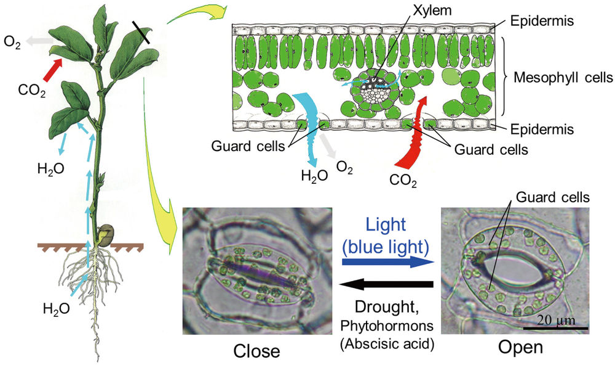
\includegraphics[width=0.8\linewidth]{figures/chap2/leaf_level_processes} 

}

\caption{Leaf level processes transpiration and photosysnthesis are strongy interlinked and both regulated by stomatal conductance}\label{fig:f21}
\end{figure}

Carbon assimilation follows two main reactions:

\begin{itemize}
\tightlist
\item
  Light harvesting (chlorophyll): the use of light to convert molecules into higher energy molecules through the photosystems
\item
  Carbon fixation: converting \(CO_2\) into sugars
\end{itemize}

The RuBisCO (ribulose-1,5-diphosphate carboxylase/oxygenase) enzyme plays an essential role for the carboxylation and oxidation reactions, while light harvesting is essential to regenerate the RuBP (ribulose 1,5-bisphosphate) --\textgreater{} see the Calvin cycle

Three different photosynthetic mechanisms:

\begin{itemize}
\tightlist
\item
  C3: PGA (phosphoglycerate) is the first product of \(CO_2\) assimilation in the Calvin cycle, the entire process takes place in the mesophyll cell
\item
  C4: PEP (phosphoenolpyruvate): make organic acids with a 4C skeleton, only 2\% of all plants follow a C4 pathway. It represents only 5 \% of the plant biomass on earth, but despite its scarcity, C4 plants account for around 23\% of the terrestrial carbon fixation; they have the Kranz anatomy, with bundle sheath cells, process is separated between mesophyll and bundle sheet cells; The main advantage is that C4 plants have a higher \(CO_2\) concentration in their bundle sheath cells, in which they also recycle \(CO_2\).
\item
  CAM: will not be discussed in the models, here the \(CO_2\) assimilation and \(CO_2\) uptake are separated in time, plants adapted to very dry conditions.
  How to observe photosynthesis? Mainly done by leaf gas exchange measurements. This methodology measures the net \(CO_2\) exchange of the leaf, which is the sum of the gross photosynthesis minus the respiration. The difference between these two fluxes is the net photosynthesis.
\end{itemize}

Photosynthesis reacts to different environmental factors (Figure \ref{fig:f22}).

\begin{enumerate}
\def\labelenumi{\arabic{enumi}.}
\tightlist
\item
  \textbf{Light}: Assimilation increases with increasing light availability, but reaches saturation at higher light levels.
\item
  \textbf{Temperature}: Assimilation increases up to an optimum temperature. Beyond the optimal temperature there is a limitation of photosynthesis.
\item
  \textbf{VPD}: Assimilation is reduced with increasing VPD.
\item
  \textbf{Moisture}: Assimilation decreases with decreasing leaf water potential (drought stress), less turgor, stomates close.
\item
  \textbf{\(CO_2\)}: Assimilation increases at elevated atmospheric \(CO_2\) concentration, with saturation.
\item
  \textbf{Nutrients}: The more nitrogen a leaf contains (for example at the top of the canopy), the more \(CO_2\) can be assimilated. Leaf N is a proxy of the amount of rubisco.
\end{enumerate}

\begin{figure}

{\centering 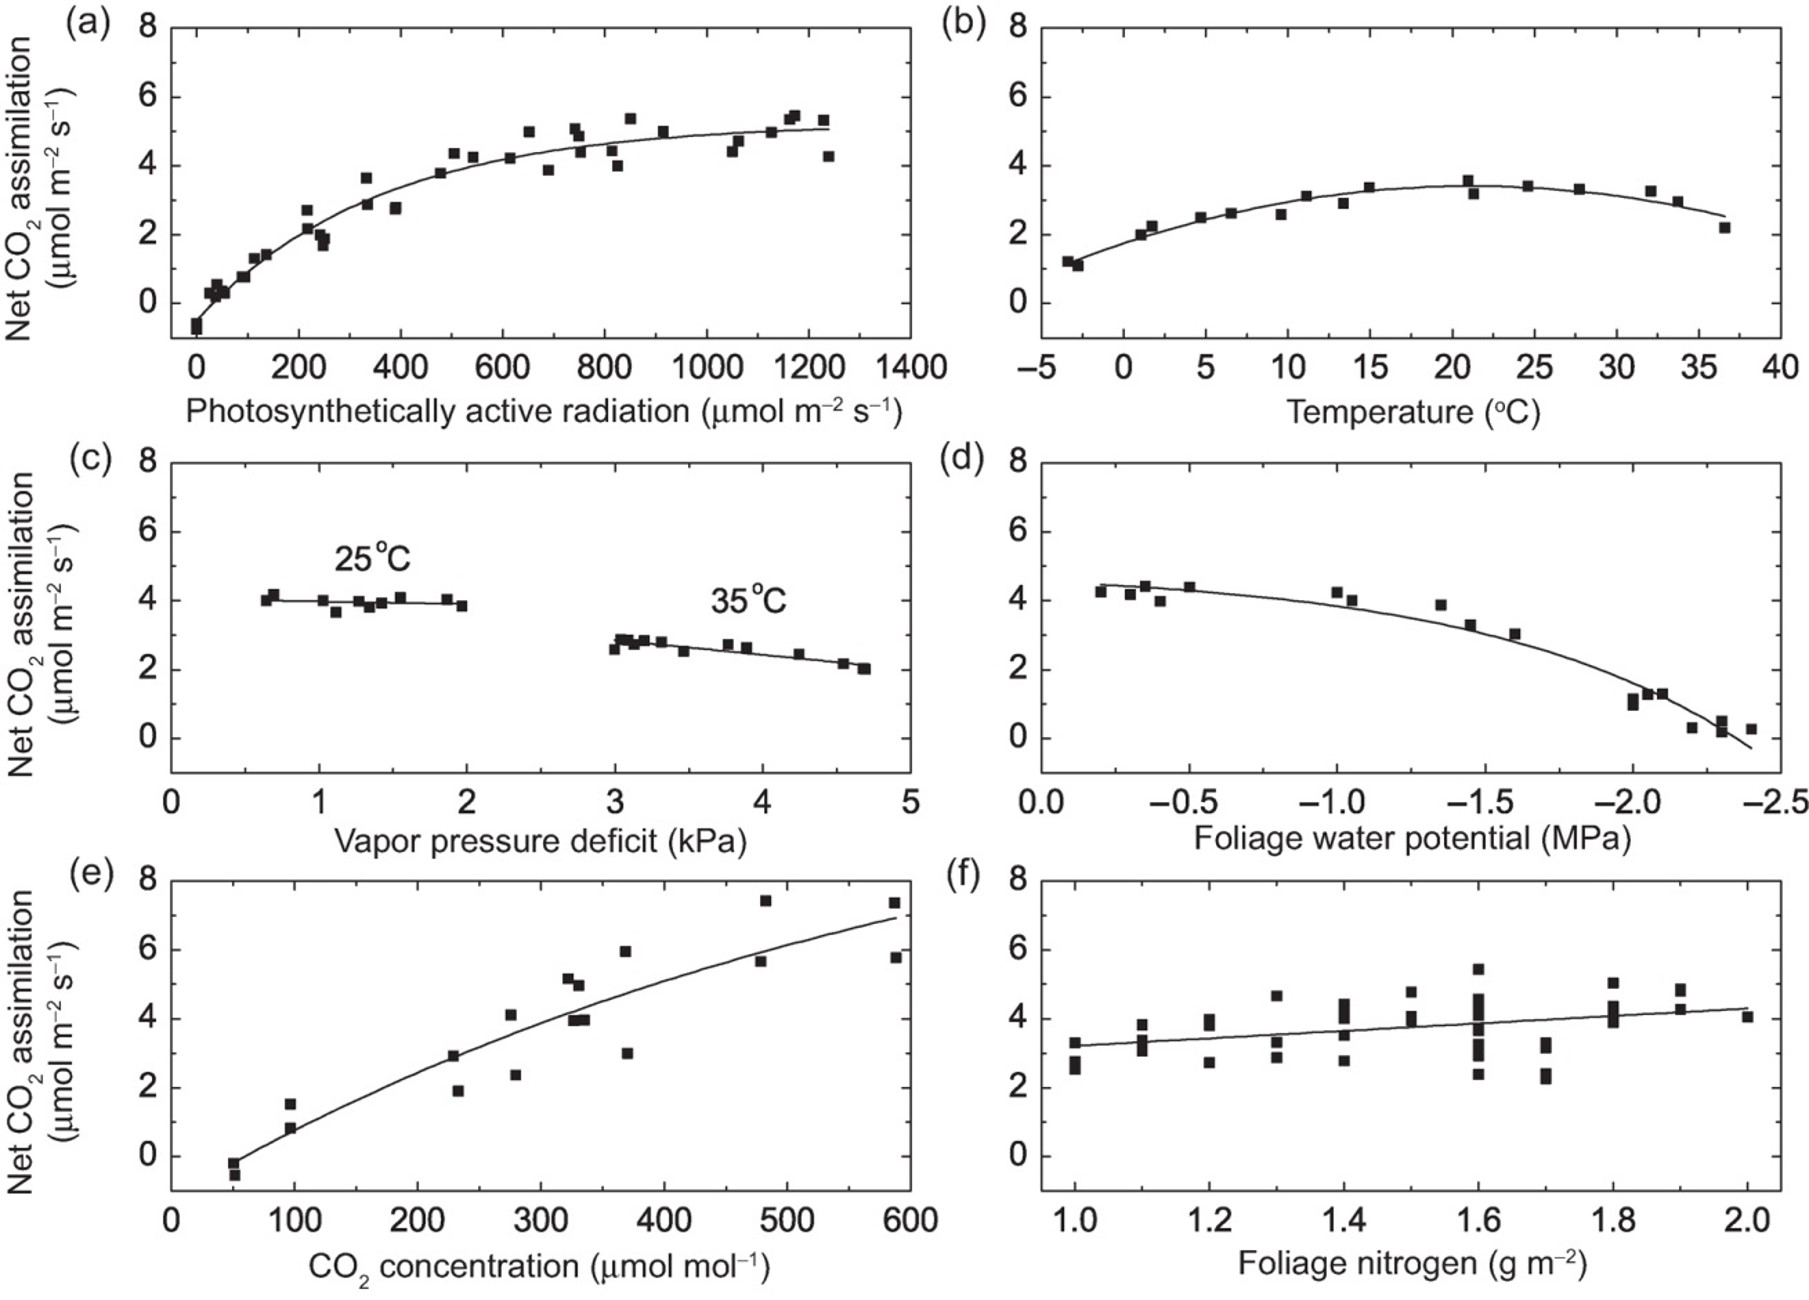
\includegraphics[width=0.8\linewidth]{figures/chap2/photosynthesis_obs} 

}

\caption{Net C assimilation in relation to (a) photosynthetically active radiation,(b) temperature, (c) vapor pressure deficit at 25°C and 35°C,(d) foliage water potential, (e) ambient $CO_2$ concentration, and (f) foliage water potential for jack pine trees (Pinus banksiana). Bonan (2019)}\label{fig:f22}
\end{figure}

Different environmental parameters interact with each other (Figure \ref{fig:f23}).

Left: leaf respiration response is different than the photosynthesis response. Respiration keeps increasing with T, followed by a collapse (degrading enzymes), the respiration peak occurs at a higher temperature than the photosynthesis peak. The temperature response is also different for different \(CO_2\) levels in the atmosphere.

Right: at lower light levels, the optimal temperature also drops. These interacting responses, need to be implemented in models!

\begin{figure}

{\centering 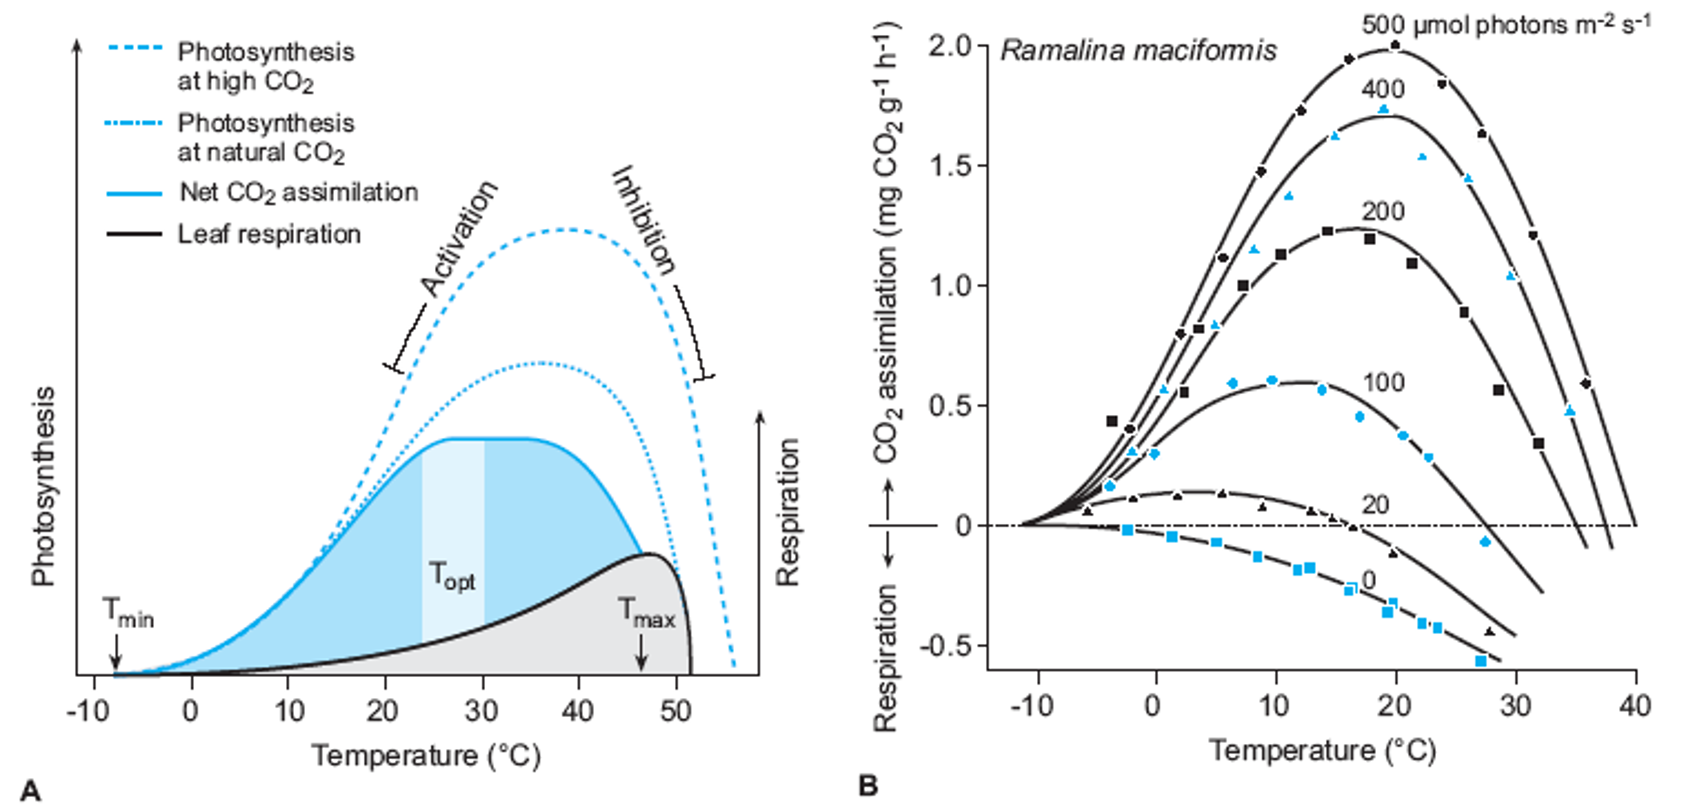
\includegraphics[width=0.8\linewidth]{figures/chap2/Trespons_interactions} 

}

\caption{Temperature responses of photosynthesis, respiration and net $CO_2$ exchange, interaction with $CO_2$ concentration (A) and light  (B)  Schulze ()}\label{fig:f23}
\end{figure}

\hypertarget{c3-photosynthesis}{%
\subsection{C3 photosynthesis}\label{c3-photosynthesis}}

\hypertarget{light-response-curve-models}{%
\subsubsection{Light response curve models}\label{light-response-curve-models}}

This model is based on light only. The slope of the curve (Figure \ref{fig:f24}) is the quantum yield, and describes the linear part of the curve.

Pmax: max photosynthesis rate, describes the level of the saturation plateau. Light compensation point, is that light level at which respiration equals the gross carbon uptake. Dark respiration: \(CO_2\) released in the dark by respiration.
This curve is described based on measurements on plants, and formulated as a mathematical equation.

\begin{figure}

{\centering 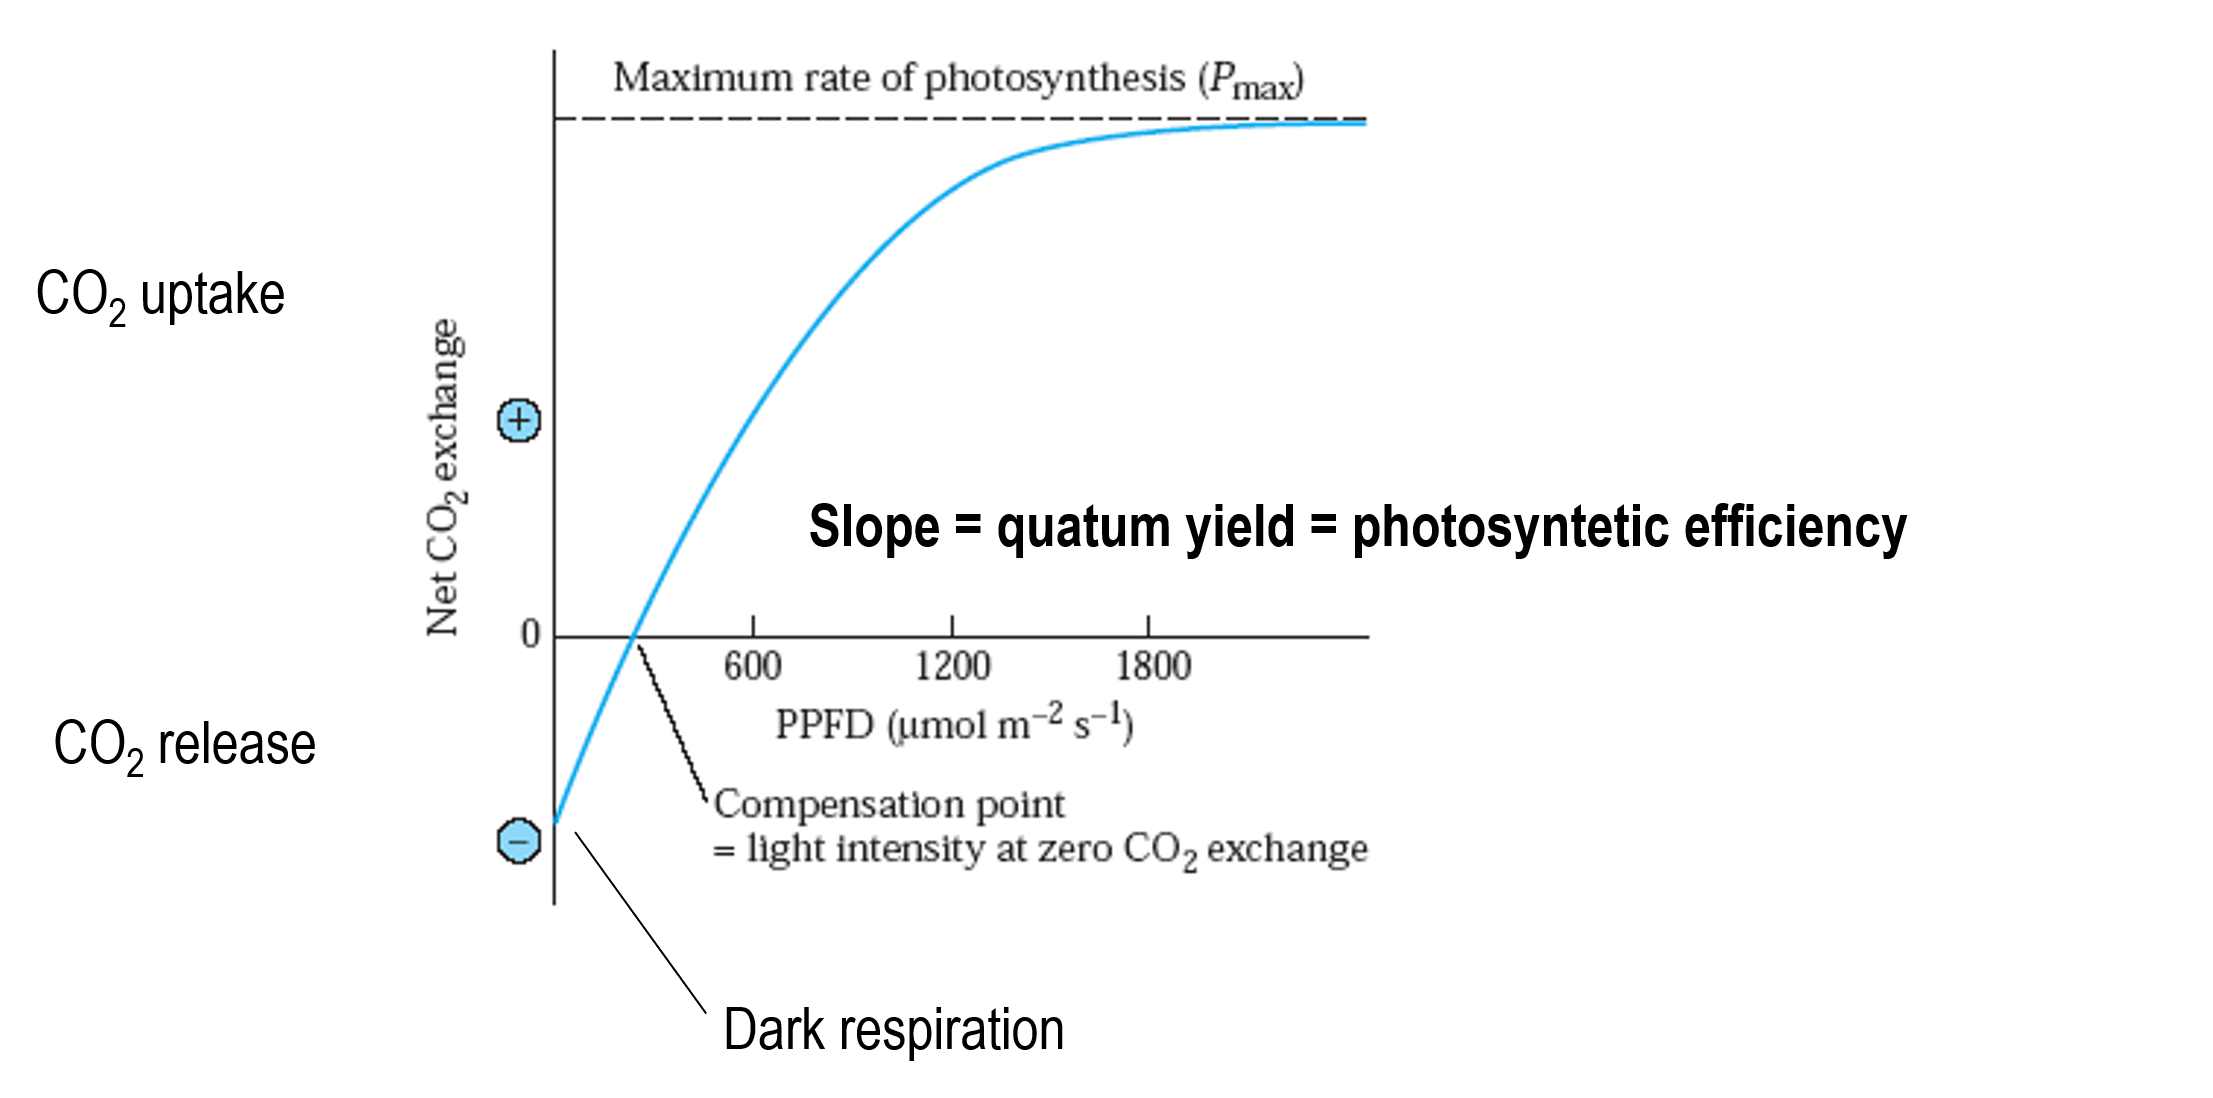
\includegraphics[width=0.8\linewidth]{figures/chap2/LRC} 

}

\caption{Conceptual figure of a leaf-level light reponse curve}\label{fig:f24}
\end{figure}

In a second approach the light response is described as a co-limitation, a response with two phases: (1) light limitation and (2) light saturation (linear increase and plateau). Such a co-limitation is described by the non-rectangulare hyperbola formula below (Figure \ref{fig:f25}). The formula has two parameters: Amax (max photosynthesis rate) and E (quantum yield). The theta factor adapts the curve shape.

Disadvantages of these light response curve models: they are measured on a specific plant in specific conditions, and only applicable under the same conditions for the same plant, on the same location. They are only used in empirical studies, not really applicable for prognostic models.

\[
\theta.A^2-(E.I+A_{max})A+E.I-A_{max}=0
\]

with \(\theta\) the curvature of the light response curve, \(A\) the assimilation rate in \(micromol m^{-2} s^{-1}\), and \(I\) the incident radiation in \(micromol m^{-2} s^{-1}\).

\begin{figure}

{\centering 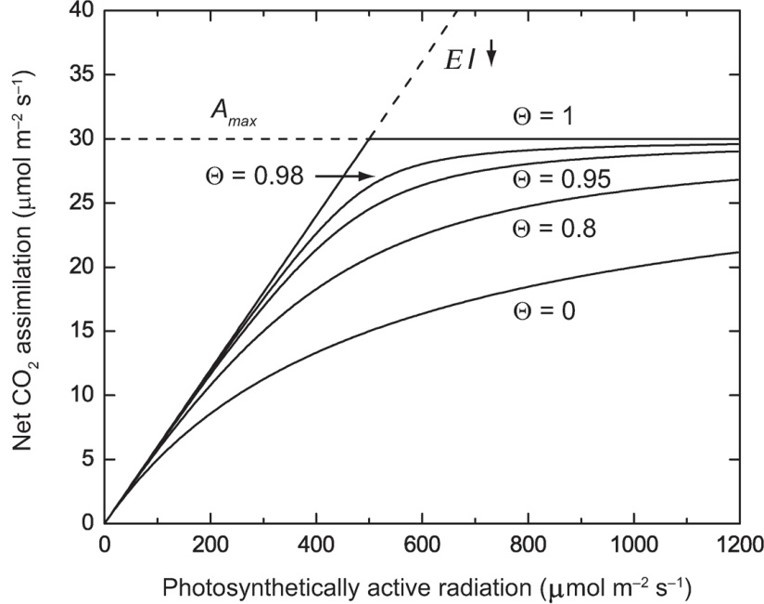
\includegraphics[width=0.8\linewidth]{figures/chap2/hyperbola} 

}

\caption{Co-limitation illustrated for photosynthetic response to light. The two dashed lines show the rates Amax adn EI The solid lines show the co-limited rate. (Bonan 2019)}\label{fig:f25}
\end{figure}

\hypertarget{light-use-efficiency-models}{%
\subsubsection{Light use efficiency models}\label{light-use-efficiency-models}}

Light use efficiency (LUE) is the slope of the linear part of the light response curve. These LUE models calculate photosynthesis at a larger scale (GPP) by multiplying the available amount of light with a light use efficiency factor(Figure \ref{fig:f26}). Other factors are introduced to mimic saturation at stressful environmental conditions (e.g.~temperature, soil water availability, atmospheric drought). These are empirical models, with its advantages and disadvantages (see above). Often used for large scale, remote sensing-based simulations of photosynthesis, as I can be measured by satellites.

\[
GPP=LUE.I.f_1(T).f_2(\theta).f_3(D)
\]

\begin{figure}

{\centering 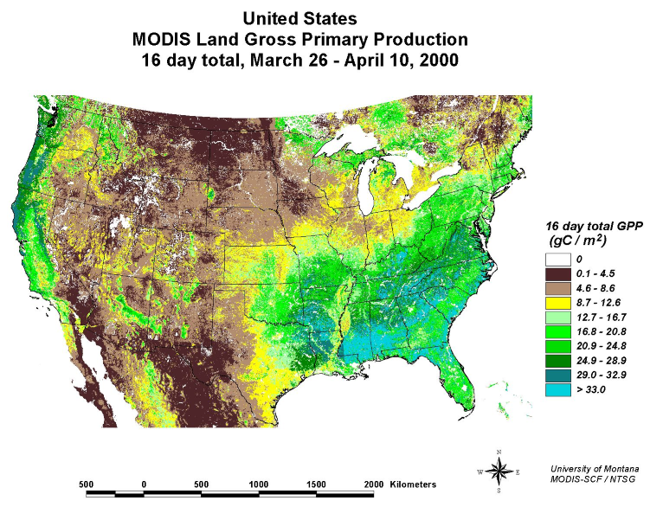
\includegraphics[width=0.8\linewidth]{figures/chap2/MODIS_GPP} 

}

\caption{MODIS based GPP map of the US, based on a LUE model.}\label{fig:f26}
\end{figure}

\hypertarget{the-farquhar-von-caemmerer-and-berry-model-fvcb}{%
\subsubsection{The Farquhar, Von Caemmerer and Berry model (FvCB)}\label{the-farquhar-von-caemmerer-and-berry-model-fvcb}}

Photosynthesis is not only limited by light response.
Diffusion of \(CO_2\) from atmosphere into the leaf plays an important role. This is driven by the \(CO_2\) concentration gradient between the atmosphere and the substomatal space. Diffusion depends on the boundary layer of the leaf, the area of the stomatal cavity as well as the resistivity of the chloroplast membrane (Figure \ref{fig:f27}).

The FvCB model was developed in 1980, and is currenty included in the large majority of (global) vegetation models. The FvCB model describes the rubisco kinetics, rubisco regeneration, the carboxylation rate when rubisco is saturated and the carboxylation rate when rubisco is limited.

\textbf{See Bonan's book, Chapter 11.1}

\begin{figure}

{\centering 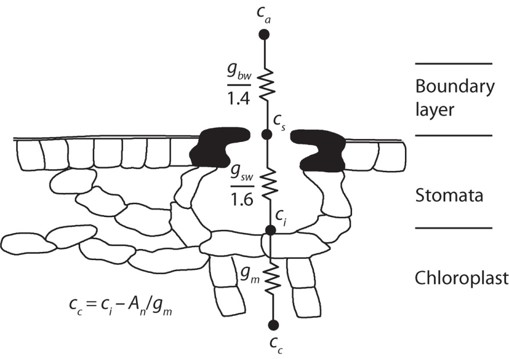
\includegraphics[width=0.8\linewidth]{figures/chap2/conductance} 

}

\caption{Diffusion of $CO_2$ from free air across the leaf boundary layer and through stomata to the intercellular space. Diffusion to the chloroplast is additionally regulated by mesophyl conductance. (Bonan 2019)}\label{fig:f27}
\end{figure}

The net photosynthesis is described as the carboxylation rate \(V_c\) minus the photorespiration \(V_o\) and dark leaf respiration \(R_d\).
\[
A_n=V_c-0.5V_o-R_d
\]
with \({A_n}\), \({V_c}\), \({Vo}\) and \({R_d}\) in \(micromol m^{-2} s^{-1}\).

\({V_c}\) corresponds to the rate of carboxylation by RUBISCO, which follows a Michalelis-Menten response function:
\[
V_c=\frac{V_{cmax}C_i}{C_i+K_c\left( 1+\frac{O_i}{K_o}\right)}
\]
with \(V_{cmax}\) the maximum rate of carboxylation in \(micromol CO_{2} m^{-2} s^{-1}\), \(C_i\) and \(O_i\) the intercellular CO\_\{2\} concentration in \(micromol mol^{-1}\), and \(K_c\) and \(K_o\) are the Michaelis-Menten constants for CO2 and O2 in \(micromol mol^{-1}\), respectively.

Photorespiration releases 0.5 mole of \(CO_2\)
\[
V_o=\frac{V_{omax}O_i}{O_i+K_o\left( 1+\frac{C_i}{K_c}\right)}
\]

It exists a specific \(C_i\) concentration value at which oxygenation compensate carboxylation and no net CO2 uptake occurs in the absence of mitrochondrial respiration. We call this value the CO2 compensation point \(\Gamma^*\). Net assimilation can be reformulated as:
\[
A_n=(1-\frac{\Gamma^*}{C_i})V_c-R_d
\]
The term \(1-\Gamma^*/C_i\) accounts for CO2 release during photorespiration.

In the simplest form of the model, carboxylation \(V_c\) is limited by either the activity of RUBISCO (CO2 limitation), denoted by the rate \(W_c\), or by the regeneration of RuBP (light limitation), denoted by the rate \(W_j\), so that:
\[
A_n=(1-\frac{\Gamma^*}{C_i})min(W_c,W_j)-R_d
\]

with Wc describing the Michealis-Menten kinetics of carboxylation.
\[
W_c=V_{cmax}\frac{C_i}{C_i+K_c(1+O_i/K_o)}
\]

and Wj represents the rate of regeneration of the RuBP by light. It depends on electron transport rate, as such the photosynthesis light response is integrated in the Farquhar model.\\
\[
W_j=J\frac{C_i}{4C_i+8\Gamma^*}
\]
\(J\) is the electron transport rate (in \(micromol m^{-2} s^{-1}\)) for a given irradiance.

The rate of electron transport is related to absorbed photosynthetically active radiation (PAR), the maximum electron transport rate and the amount of light utilized by photosystems. Different expressions can be found for J. We will use the most common form:

\[
J=\frac{I_{abs}+J_{max}-\sqrt{(I_{abs}+J_{max})^2-4\theta_jI_{abs}J_{max}}}{2\theta_j}
\]

with \(I_{abs}\) the absorbed PAR in \(micromol photon m^{-2} s^{-1}\), \(\theta_j\) is the curvature of the light response curve and \(J_{max}\) the maximal electron transport rate in \(micromol m^{-2} s^{-1}\).

The absorbed incident radiation by the photosystem II (\(I_{abs}\)) depends on leaf absorptance \(\alpha_l\) and the quantum yield of photosystem II \(\phi_{PSII}\):
\[
I_{abs}=\frac{\phi_{PSII}}{2}\alpha_lI_r
\]
where \(I_r\) is PAR in \(micromol m^{-2} s^{-1}\), and only one half of absorbed light reaches the PSII.

In summary, a common form of the FvCB model represents photosynthetic CO2 assimilation for plants utilizing the C3 photosynthetic pathway as limited by (i) Ac -- the rate of Rubisco catalyzed carboxylation when RuBP is saturated (called Rubisco-limited photosynthesis because of its dependence on maximum Rubisco activity as set by Vcmax); and (ii) Aj -- the rate of RuBP regeneration by light absorption and electron transport as determined by Jmax (RuBP regeneration-limited, or light-limited, photosynthesis).

When accounting for the CO2 compensation point, the general Farquhar model is thus written as follows:

\[
A_n=min(A_c,A_j)-R_d
\]
with
\[
A_c = V_{cmax}\frac{C_i-\Gamma^*}{C_i+K_c\left(1+\frac{O_i}{K_c}\right)}
\]

\[
A_j = \frac{J}{4}\left(\frac{C_i-\Gamma^*}{C_i+2\Gamma^*}\right)
\]

Figure \ref{fig:f28} illustrates the response of assimilation to intercellular \(CO_2\) and light. We neglect TPU limitation (\(A_p\)) in the models we consider here. TPU limitation only occurs at elevated intercellular \(CO_2\).

\begin{figure}

{\centering 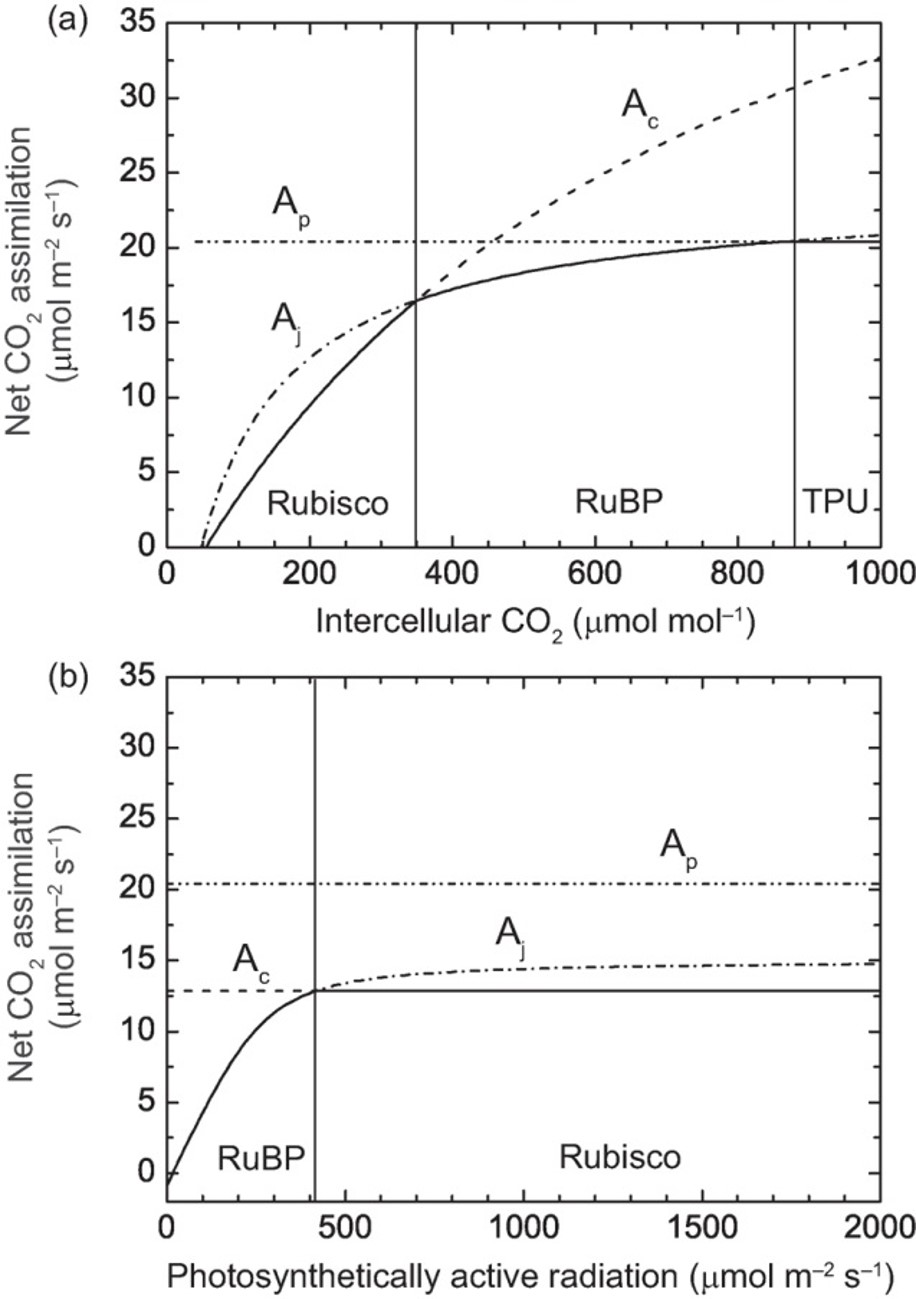
\includegraphics[width=0.8\linewidth]{figures/chap2/simulated_responses} 

}

\caption{Simulated responses of C3 photosynthesis in relation to (a) intercellular $CO_2$ (at I↓ = 2000 micromol m–2 s–1) and (b) photosynthetically active radiation (at ci = 266 micromol mol–1). (Bonan 2019)}\label{fig:f28}
\end{figure}

As an alternative formulation a co-limitation analytical model can be used. In this case we don't use the minimum equation of the original Farquhar model, but take both limitations into account simultaneously in the following equation.

\[
\Theta_{A}A^2-(A_c+A_j)A+A_cA_j
\]

\hypertarget{parameter-and-temperature-dependencies}{%
\subsection{Parameter and temperature dependencies}\label{parameter-and-temperature-dependencies}}

\textbf{See Bonan's book, Chapter 11.2}

The FvCB model requires 6 physiological parameters: \(K_c\), \(K_o\), \(\Gamma^*\), \(V_{cmax}\), \(J_{max}\) and \(R_d\). Additionally, the specification of electron transport requires \(\theta_j\) and \(\phi_j\). Values for\(K_c\), \(K_o\) and \(\Gamma^*\) are defined by the biochemistry of Rubisco and are similar among species. On the opposite, \(V_{cmax}\) is species-dependent.

\(V_{cmax}\) is a key parameter in the FvCB model. It directly determines the Rubisco-limited rate \(A_c\) and, for C3 plants, also influences the RuBP regeneration-limited rate \(A_j\) though its covariation with \(J_max\). The maximum rate of carboxylation has a wide range among plant species and environments and is tightly linked to leaf nitrogen content; reported values for 109 species of C3 plants vary from less than 10 to more than 150 \(micromol m^{–2} s^{–1}\).

Because \(J_{max}\) is well correlated to \(V_cmax\), it can be approximated to:
\[
J_{max} = 1.67V_{cmax}
\]

\(R_d\) is also well correlated to \(V_cmax\) and can be approximated as:
\[
R_d=0.015V_{cmax}
\]

The parameters \(K_c\), \(K_o\), \(\Gamma^*\), \(V_{cmax}\), \(J_{max}\) and \(R_d\) vary with temperature (Figure \ref{fig:f28bis}). The instantaneous responses of photosynthesis and respiration to temperature are driven by their underlying enzymatic responses. When warmed from low temperature, the enzymes involved in photosynthesis and respiration increase their activity as described by the Arrhenius function:
\[
f(T_l)=exp\left[\frac{\Delta H_a}{298.15R}(1-\frac{298.15}{T_l})\right]
\]
where \(T_l\) is leaf temperature (in K), R is the universal gas constant (8.314 J K\textsuperscript{--1} mol\textsuperscript{--1}), and \(\Delta H_a\) is the activation energy (J mol\textsuperscript{--1}). This function is normalized to 25°C (298.15 K). Parameter values measured at 25°C are multiplied by \(f(T_l)\) to adjust for leaf temperature.

\begin{figure}

{\centering 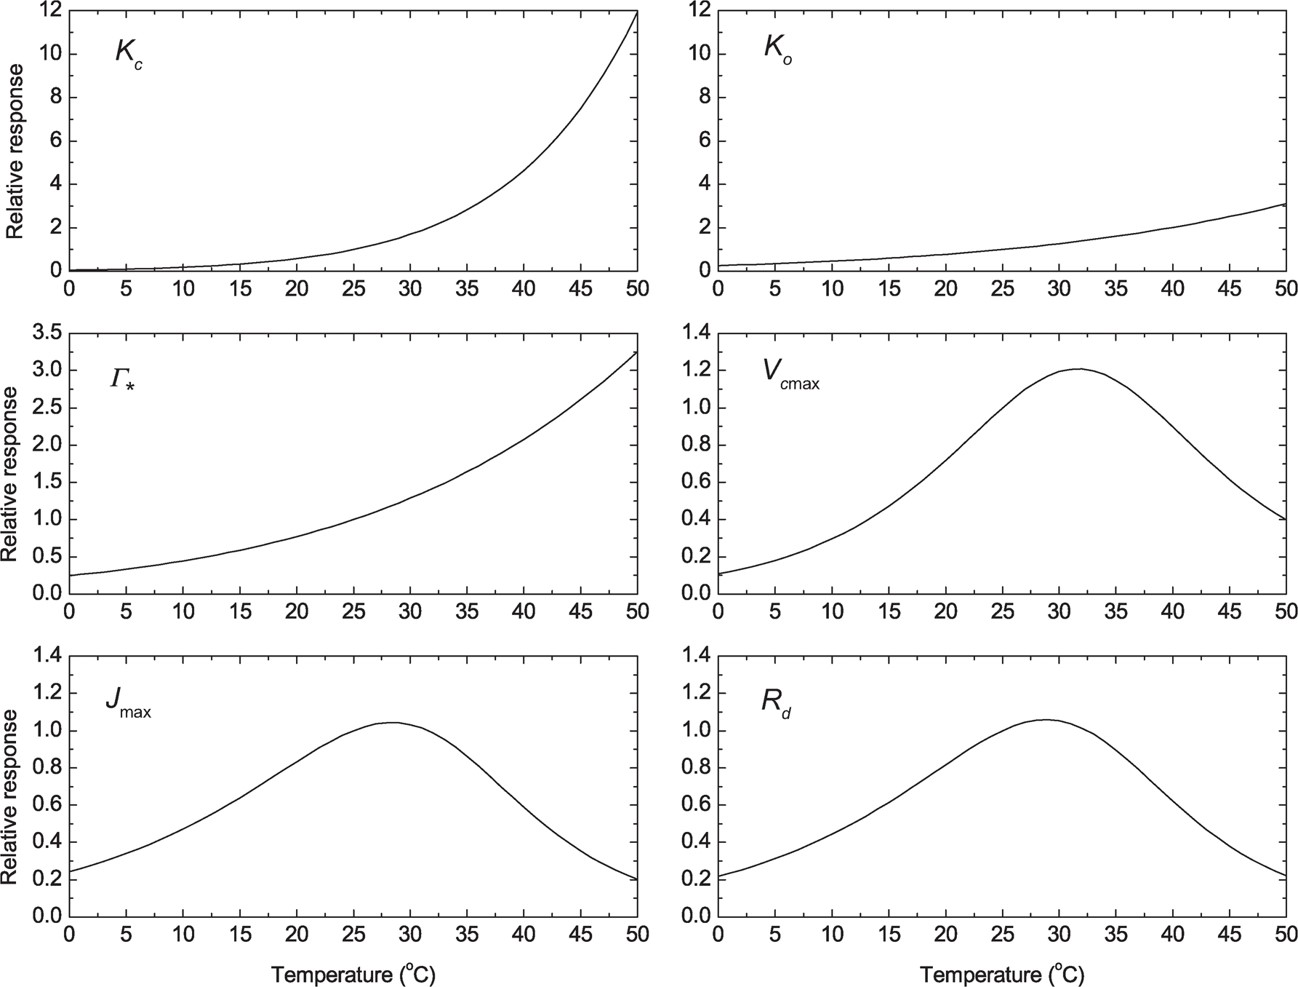
\includegraphics[width=0.8\linewidth]{figures/chap2/temp_responses} 

}

\caption{Relative temperature responses of the parameters of the Farquhar model (Bonan 2019)}\label{fig:f28bis}
\end{figure}

The parameters \(V_{cmax}\), \(J_{max}\) and \(R_d\) vary with temperature following the Arrhenius function but have a peaked response in which enzymatic activity increases up to a temperature optimum beyond which the reaction rate decreases when temperature is too high because of enzyme degradation. In this case, parameters such as \(V_{cmax}\) are writen by:
\[
V_{cmax}=V_{cmax25}f(T_l)f_H(T_l)
\]
with \(V_{cmax25}\) the value of \(V_{cmax}\) at 25°C. The \(f_H(T_l)\) function represents the thermal breakdown of biochemical processes:
\[
f_H(T_l)=\frac{1+exp\left(\frac{298.15\Delta S-\Delta H_d}{298.15R}\right)}{1+exp\left(\frac{\Delta ST_l-\Delta H_d}{RT_l}\right)}
\]

To correctly model photosynthesis over time, you should also take into account climate adaptation (acclimation): the temperature adaptation curve is different for the same species if they are grown under different climatic conditions.

Challenges with the Farquhar model: its parameter values are not well defined, or the values of the parameters are highly variable, depending on the type of plant or environmental conditions. Vcmax is highly variable over different leaves in the same tree, and on global scales.
Which value should we use? -\textgreater{} Vcmax is scaling very well to photosynthesis, so Vcmax is often optimized with data available. However, by doing so you turn the model into an empirical model, so this should be avoided.
The advantage we have, is that there are covariations between parameters (Figure \ref{fig:f29}) for example the strong correlation between Vcmax and Jmax -\textgreater{} you can describe Jmax as a function of Vcmax, so you can remove one parameter from the model.

\begin{figure}

{\centering 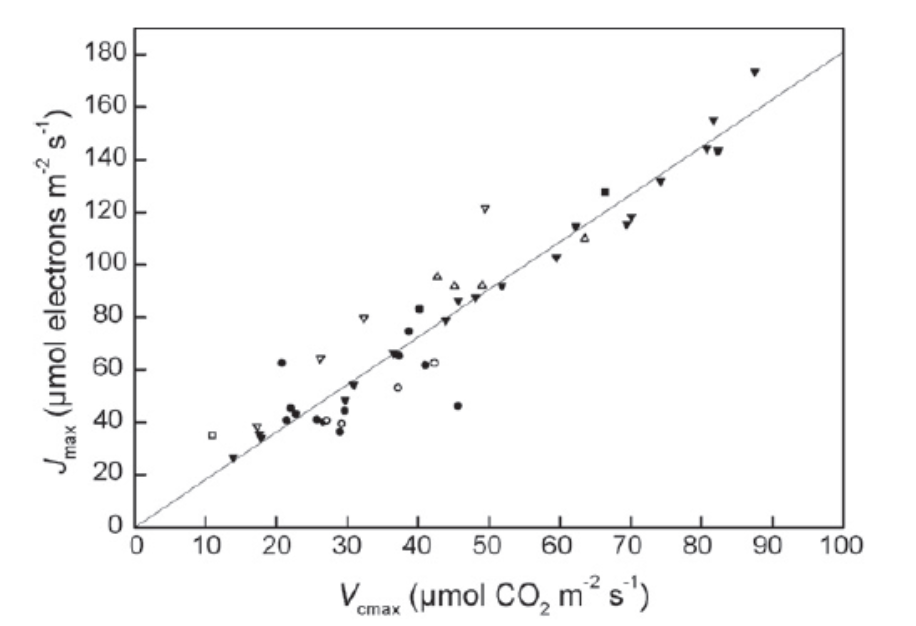
\includegraphics[width=0.8\linewidth]{figures/chap2/vcmax_jmax} 

}

\caption{Linear relation between observed Vcmax and Jmax values for Beech (Verbeeck et al. 2008)}\label{fig:f29}
\end{figure}

Vcmax can also be calculated based on leaf nitrogen content. Some vegetation models model the N content of leaves, and simulated based on the Vcmax of the leaves. It's a linear relationship with two parameters. Some models also use more complex relations.

There are also attempts to propose average values per plant functional type.

\[
V_{cmax25} = i_v + s_v.N_a
\]
The temperature functions also have dependence factors.

The Farquhar model has 4 input variables: \(O_i\), \(C_i\), \(PAR\) and \(T_{leaf}\). Light depends on how the radiation is penetrating the canopy \textbf{-\textgreater{} see lecture 3}. \(O_i\) is assumed to be equal to the oxygen concentration in the atmosphere. Leaf temperature \(T_{leaf}\) is in most models assumed to be equal to air temperature or can be calculated based on an energy balance. \(C_i\) is calculated based on gas diffusion through the stomates -\textgreater{} you need an extra model to fully simulate the behavior of the stomates.

\begin{figure}

{\centering 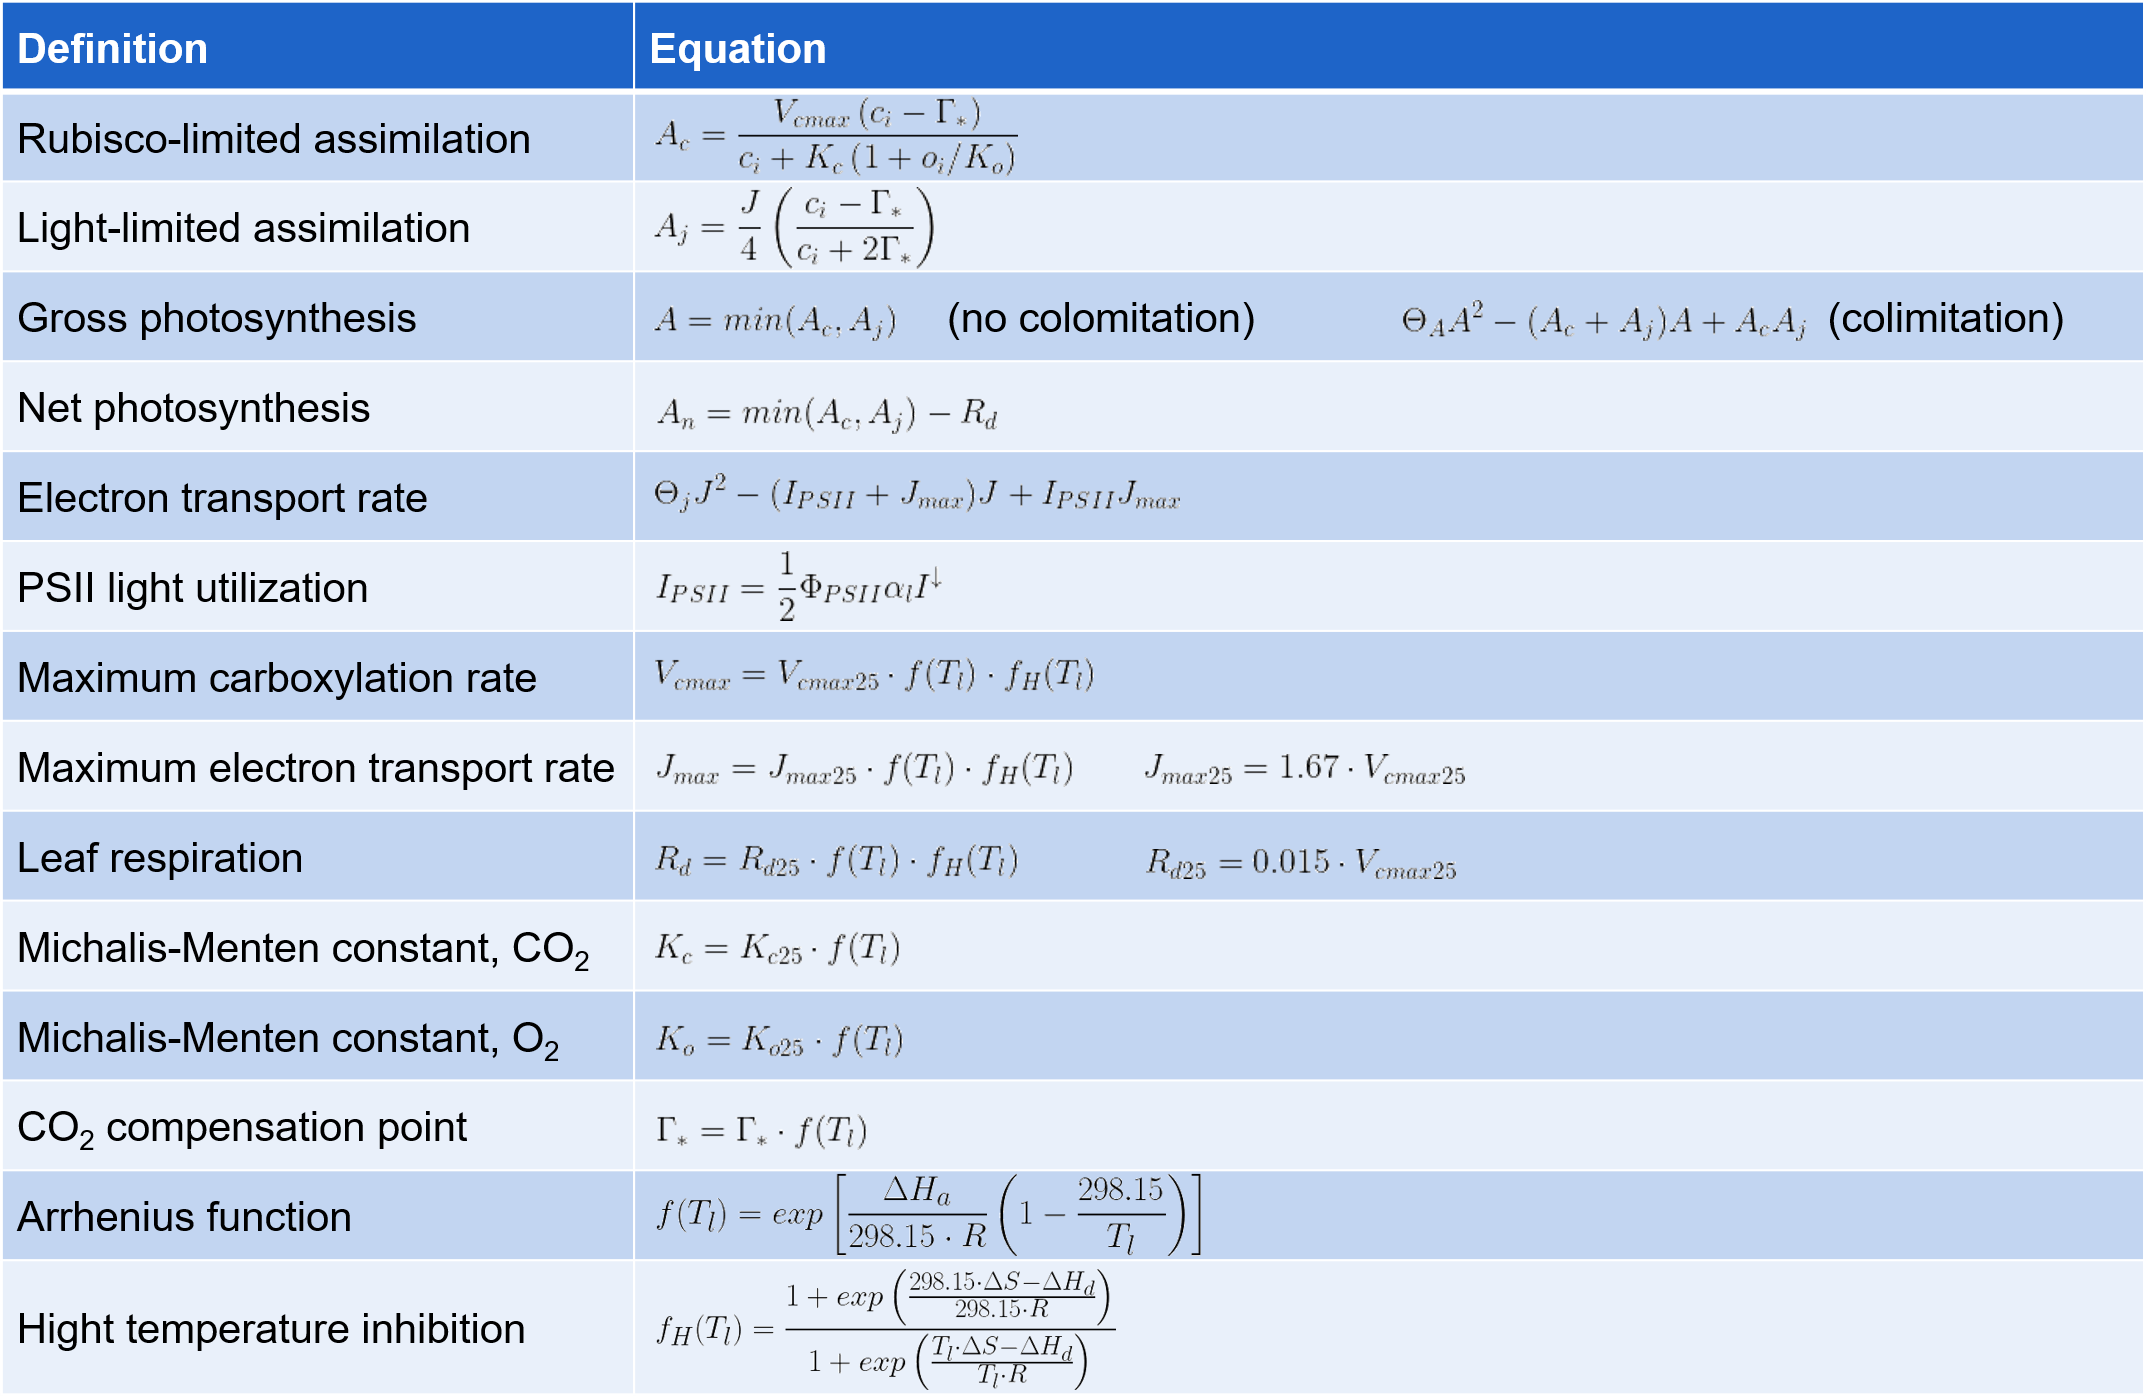
\includegraphics[width=0.8\linewidth]{figures/chap2/full_farquhar} 

}

\caption{Equations of the full Farquhar model}\label{fig:f210}
\end{figure}

\hypertarget{c4-photosynthesis}{%
\subsection{C4 photosynthesis}\label{c4-photosynthesis}}

\textbf{See Bonan's book, Chapter 11.7}

The behaviour of the C4 and C3 models is really different

\begin{figure}

{\centering 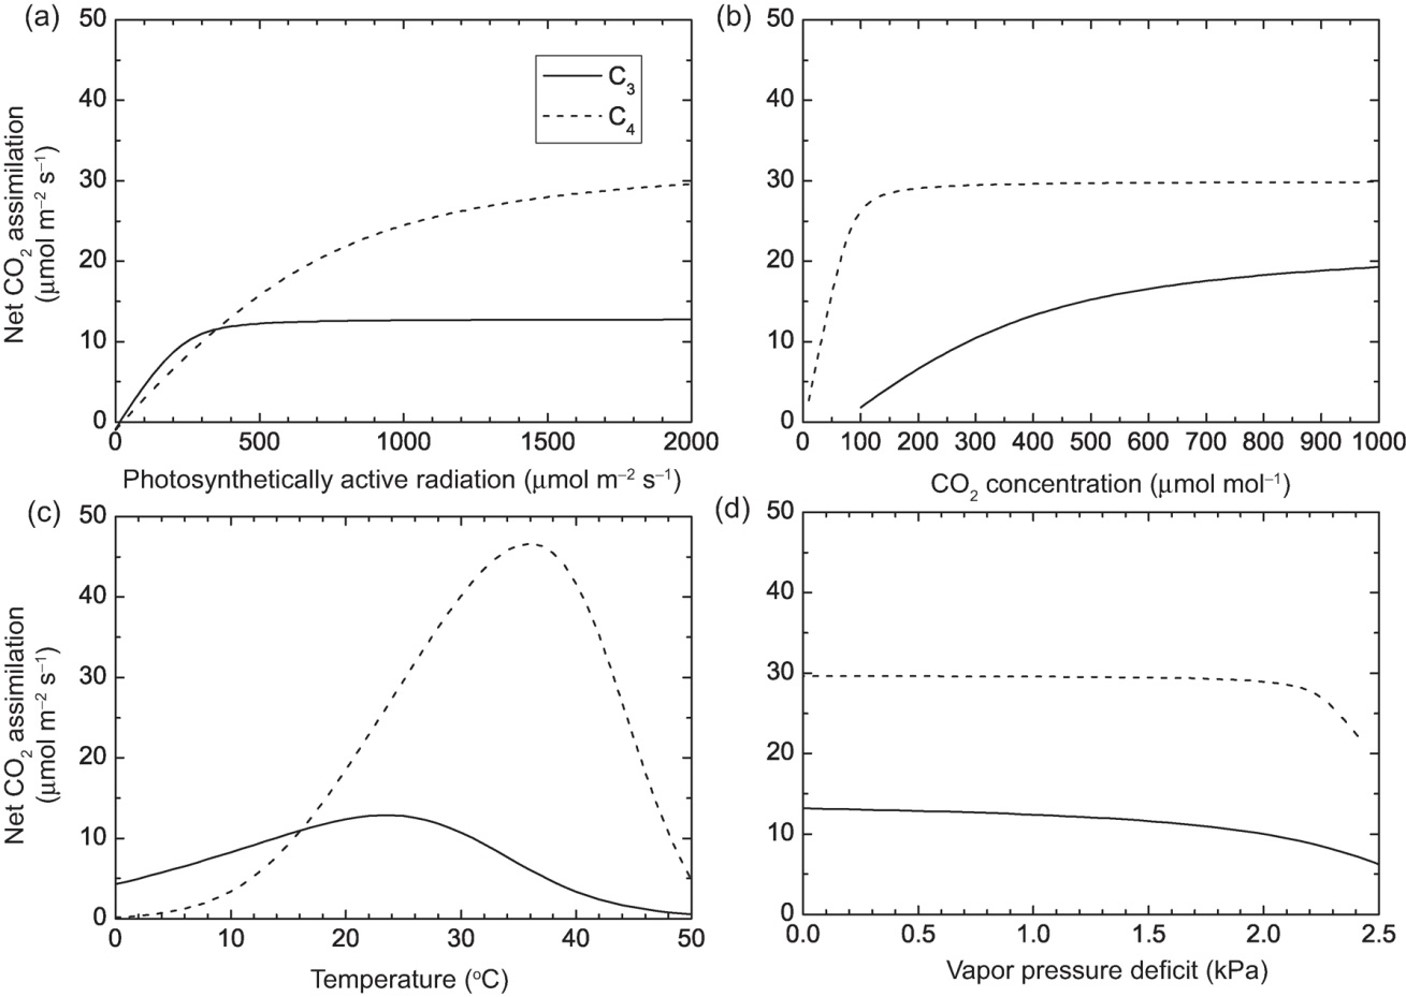
\includegraphics[width=0.8\linewidth]{figures/chap2/c3_c4} 

}

\caption{Comparison of C3 and C4 photosynthesis in response to (a) photosynthetically active radiation, (b) ambient $CO_2$ concentration, (c) leaf temperature, and (d) vapor pressure deficit. In this figure, stomatal conductance is calculated using the Ball–Berry model and ci is obtained from the diffusion equation}\label{fig:f210b}
\end{figure}

\hypertarget{stomatal-models}{%
\section{Stomatal models}\label{stomatal-models}}

\hypertarget{refreshing-the-basic-knowledge-1}{%
\subsection{Refreshing the basic knowledge}\label{refreshing-the-basic-knowledge-1}}

Guard cells are transporting ions actively and passively into/out of the cells in order to open or close the stomates by adapting the turgor in the guard cells.
The stomatal conductance represents how easy it is for a \(CO_2\) molecule to diffuse in or out of the stomates. The higher the conductance, the easier the transfer.
Stomatal models are needed for transpiration, leaf temperature and \(CO_2\) -\textgreater{} key process in the model. Stomatal conductance for \(CO_2\) is lower than that of water as the molecule is a bit bigger. Sometimes expressed as a resistance in models that use the electric analog concept (Figure \ref{fig:f211}).

\begin{figure}

{\centering 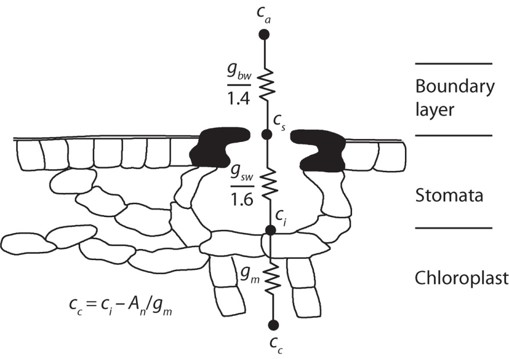
\includegraphics[width=0.8\linewidth]{figures/chap2/conductance} 

}

\caption{Diffusion of $CO_2$ from free air across the leaf boundary layer and through stomata to the intercellular space. Diffusion to the chloroplast is additionally regulated by mesophyl conductance. (Bonan 2019)}\label{fig:f211}
\end{figure}

Plants constantly balance their physical and biochemical limitation, by adjusting their stomatal conductance.

Photosynthesis is expressed as a diffusion process. Photosynthesis flux is a range through the circuit of figure \ref{fig:f211}. \(A_n\) can be described as the flux going from the atmosphere to the internal part of the leaf, or as the flux going from the internal part of the leaf into the cell, or a combinations of the two methods.

\[
A_n=\frac{g_{bw}}{1.4}(C_a-C_s) = \frac{g_{sw}}{1.6}(C_s-C_i)=\frac{1}{1.4g_{bw}^{-1}+1.6g_{sw}^{-1}}(C_a-C_i)
\]
with \(g_{sw}\) and \(g_{bw}\) the stomatal and boundary layer conductance for water, respectively, in mol m\textsuperscript{-2} s\textsuperscript{-1}. the ratio 1.6 correspond to the molecular mass ration between \(H_2O\) and \(CO_2\) to convert conductance to water to \(CO_2\). \(C_a\), \(C_s\) and \(C_i\) are the \(CO_2\) concentration from the atmosphere, at leaf surface and in the stomatal cavity, respectively.

Stomatal conductance is also dependent on environmental conditions (Figure \ref{fig:f212}). There is a saturated response to light, an optimum for temperature, strong response to VPD, stomata close when VPD is too high, and there is a response to the leaf water potential. Again, there is interaction between the different environmental conditions.

\begin{figure}

{\centering 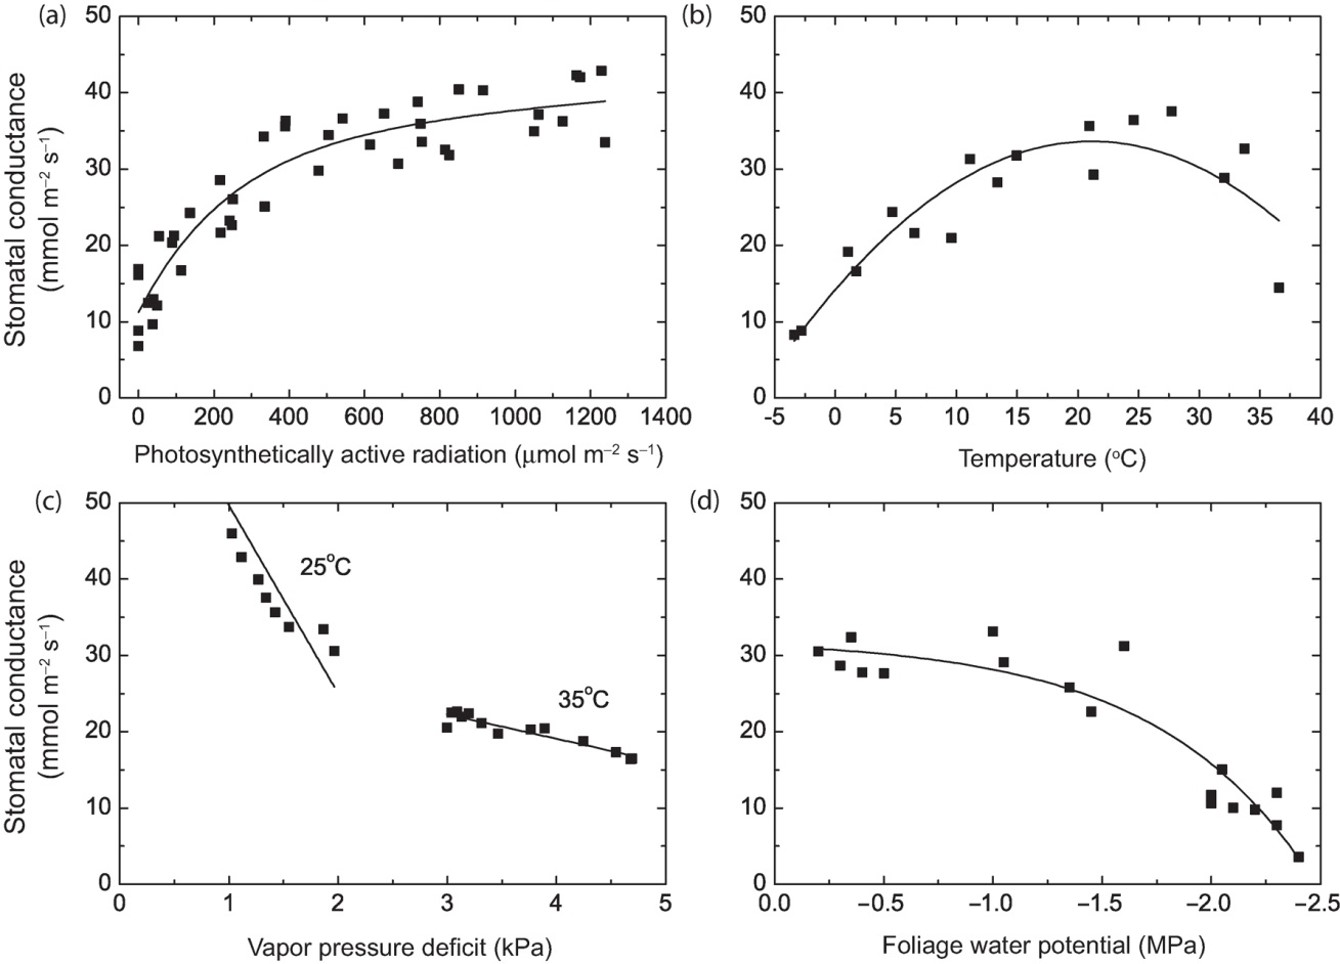
\includegraphics[width=0.8\linewidth]{figures/chap2/gs_obs} 

}

\caption{Observed responses of stomatal conductance for Pinus banksiana. (Bonan 2019)}\label{fig:f212}
\end{figure}

If the air is dry stomates close to avoid losing too much water

\emph{accounting for all these effects makes it complex
}stomatal conductance is quite linear with photosynthesis

We have three unknowns in the combined photosynthesis-diffusion equations but only two equations: we need an extra equation to describe stomatal conductance to be able to solve for the unknowns. 4 Possibilities discussed: see below.

\hypertarget{empirical-multiplicative-models}{%
\subsection{Empirical multiplicative models}\label{empirical-multiplicative-models}}

This is an empirical approach. The actual stomatal conductance is calculated based on the max stomatal conductance (\(G_{smax}\) multiplied by correction factors for light, temperature, etc. between 0 and 1. It is based on observations. Gsmax is species dependent.
There is no link with the carbon cycle/photosynthesis, this is why it is not used anymore in the global vegetation models as part of the earth system models of the IPCC

\[
g_{sw}=g_{smax}f(I^{\downarrow})f(T_l)f(D_l)f(\Phi_l)f(C_a)
\]

\hypertarget{semi-empirical-photosynthesis-based-models}{%
\subsection{Semi-empirical photosynthesis-based models}\label{semi-empirical-photosynthesis-based-models}}

Semi-empirical models are still commonly used in vegetation models and are based on the linear relation between stomatal conductance and photosynthesis (Figure \ref{fig:f213}).

\begin{figure}

{\centering 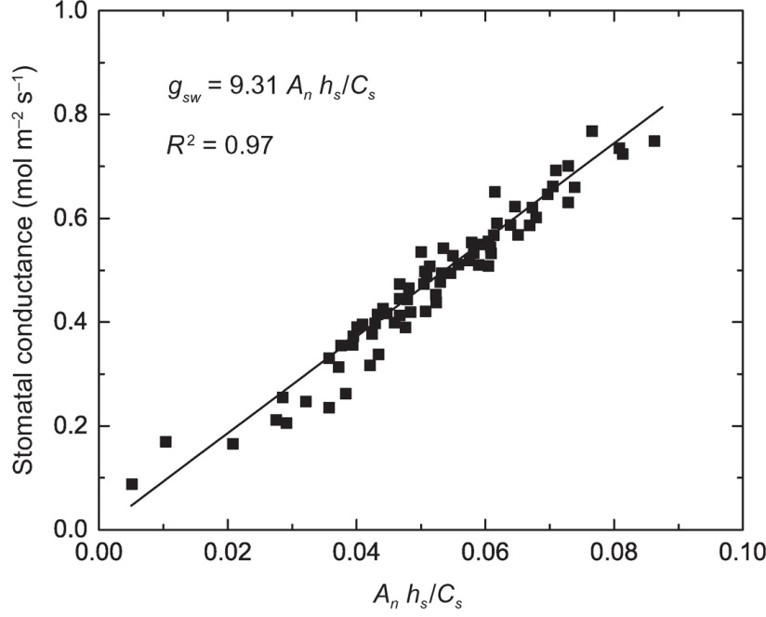
\includegraphics[width=0.8\linewidth]{figures/chap2/ball_berry} 

}

\caption{Relationship between stomatal conductance and Anhs/cs for soybean.(Bonan 2019). On the x axis, the photosynthesis is depicted, but multiplied by relation humidity and $CO_2$ concentration at the leaf surface.}\label{fig:f213}
\end{figure}

\textbf{Ball-Berry model}: Stomatal conductance is calculated based on photosynthesis, relative humidity and \(CO_2\) concentration at the leaf level. This is the third equation needed to solve the problem. The model needs observations to determine the parameters (i.e.~semi-empirical).
Plants adapt their stomatal opening to maintain a constant Ci/Ca ratio, or the \(CO_2\) concentration in the leaf and the concentration outside the leaf (atmosphere).
As the model uses the \(CO_2\) concentration at the surface of the leaf, we also need the boundary layer conductance.

\[
g_{sw}=g_0 + g_1\frac{A_n}{C_s}h_s
\]
with \(g_0\) and \(g_1\) empirical model parameters, \(A_n\) the net assimilation, \(C_s\) the \(CO_2\) concentration at the leaf surface and \(h_s\) the relative air humidity.

The model becomes a combination of multiple non-linear equations, which cannot be solved analytically. Some model try to find an analytical solution by simplifying the equations, this gains calculation speed. Other models use numerical techniques based on the scheme below (Figure \ref{fig:f214}): we start with an initial guess of \(C_i\) and do enough iterations until the guess convergences with the outcome value of the model. This approach is slower as multiple iterations have to be calculated, which is time-consuming.
This model still needs empirical input to determine the Ball-Berry parameters. SO it is a theoretical model that needs empirical constraints.

\begin{figure}

{\centering 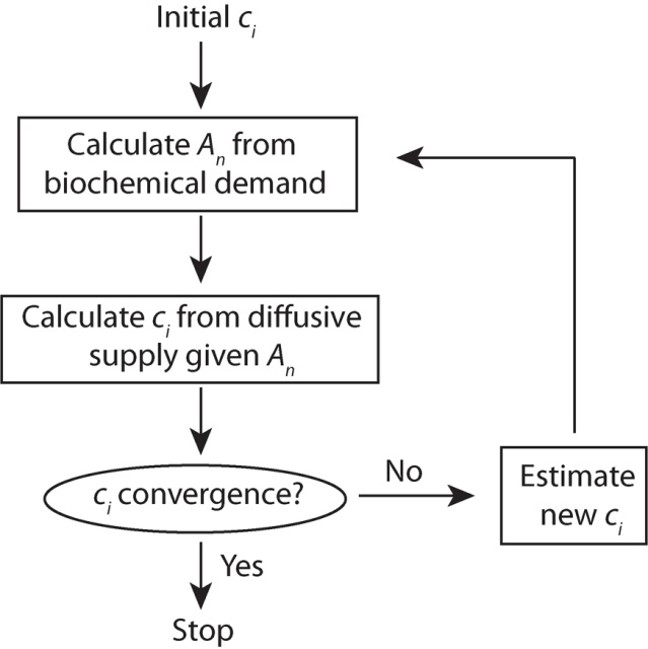
\includegraphics[width=0.8\linewidth]{figures/chap2/numerical_solution} 

}

\caption{Flow diagram of the iterative procedure to numerically calculate ci.(Bonan 2019)}\label{fig:f214}
\end{figure}

\hypertarget{wue-models-and-optimality-theory}{%
\subsection{WUE models and optimality theory}\label{wue-models-and-optimality-theory}}

Not discussed in detail, but this approach is increasingly implemented in models as it overcomes the use of empirical parameters. They are based on ecological theories. Here, the stomatal conductance is optimized by maximizing the water use efficiency. We assume that plants try to optimize the benefit of photosynthesis with the cost of water loss. Stomatal conductance is not described explicitly by an equation, but it emerges from the model.
The concept of calculations is shown in figure \ref{fig:f215}: we start with an assumed stomatal conductance value, we go through all calculations and in the end calculate WUE and do the same for an increased/decreased stomatal conductance, and check what the gain of WUE is.

\begin{figure}

{\centering 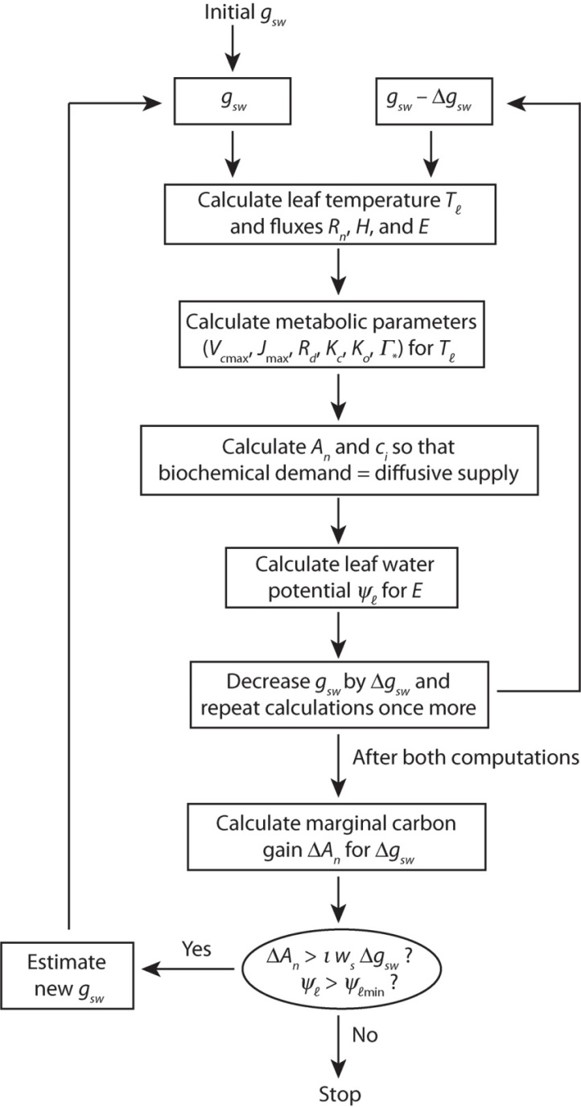
\includegraphics[width=0.8\linewidth]{figures/chap2/optimality} 

}

\caption{Flow diagram of leaf flux calculations to numerically solve for stomatal conductance that optimizes water-use efficiency.(Bonan 2019)}\label{fig:f215}
\end{figure}

\hypertarget{soil-drought-stress}{%
\subsection{Soil drought stress}\label{soil-drought-stress}}

Basic models do not account for soil drying. Many models add an additional factor that describes the soil wetness. The beta factor varies between 0 (wilting point) and 1 (field capacity), with different courses between the two extremes (see figure \ref{fig:f216}). Various vegetation models differ in the way they account for this factor. Some models apply this factor on Vcmax other model integrated the factor in the stomatal equation.
Some models simulate leaf figure (Figure \ref{fig:f216}) or soil (Figure \ref{fig:f217}) water potentials. Species have a different response to the leaf water potential. First there is no impact, species have a tolerance, but after threshold, a decrease in photosynthesis occurs.

\begin{figure}

{\centering 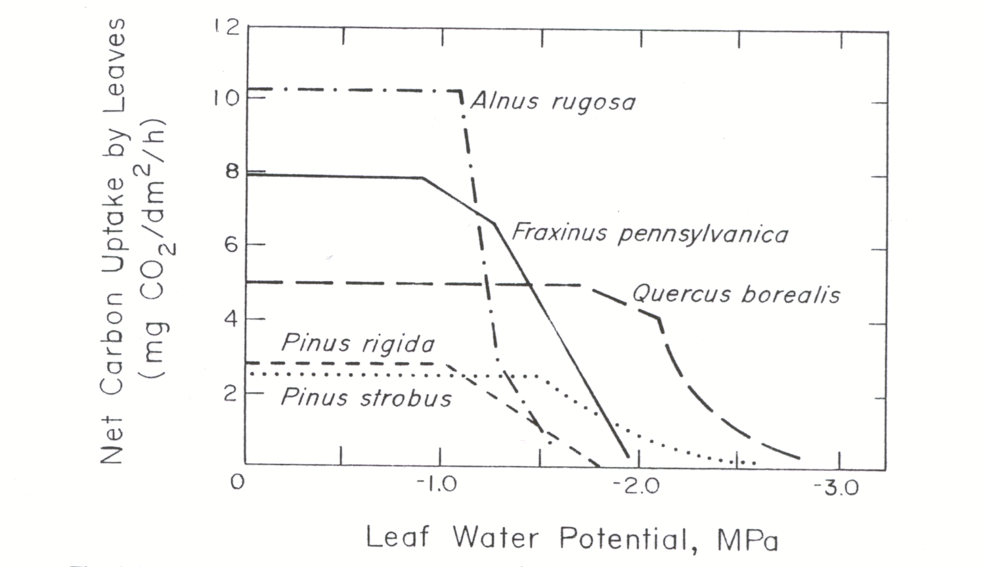
\includegraphics[width=0.8\linewidth]{figures/chap2/leafWP} 

}

\caption{Leaf carbon uptake in response to leaf water potential for multiple tree species.}\label{fig:f216}
\end{figure}

\begin{figure}

{\centering 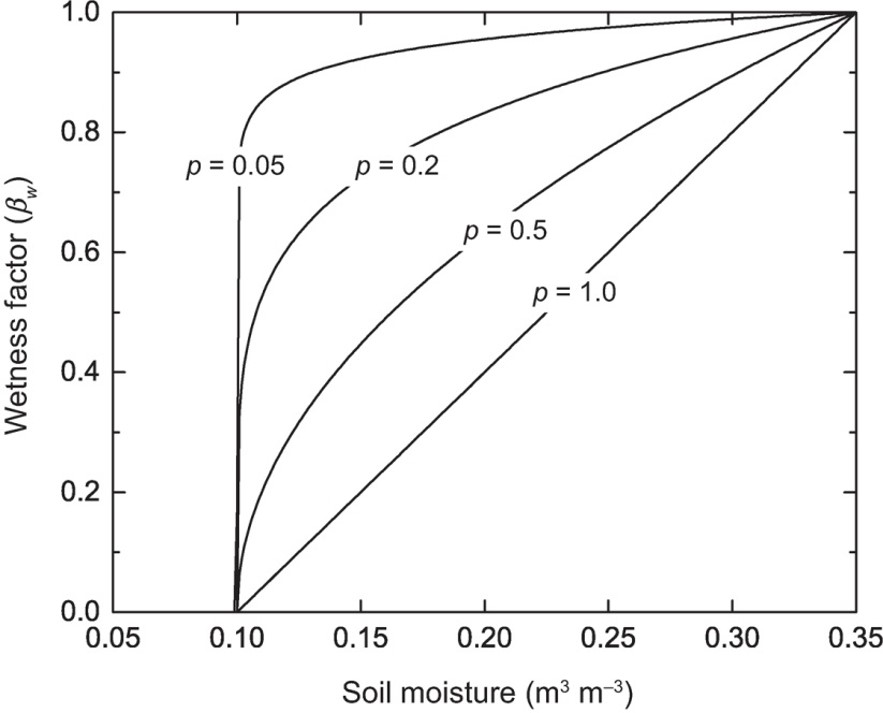
\includegraphics[width=0.8\linewidth]{figures/chap2/SWfactor} 

}

\caption{Soil moisture wetness factor in relation to volumetric water content. (Bonan 2019)}\label{fig:f217}
\end{figure}

\hypertarget{hydraulic-models}{%
\subsection{Hydraulic models}\label{hydraulic-models}}

These models are originally developed to simulated plant water relations of individual plants/trees (Figure \ref{fig:f218}). The model simulates the water transport through the trees. Challenging to apply at the large scale.
Isohydric species: maintain their leaf water potential, independently from the soil water potentials.

\begin{figure}

{\centering 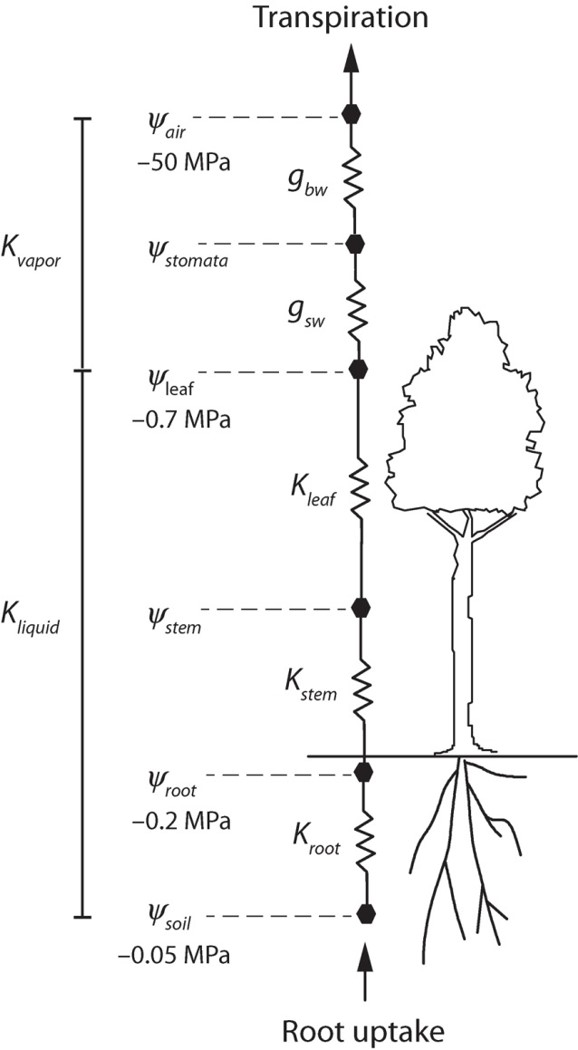
\includegraphics[width=0.8\linewidth]{figures/chap2/hydraulics} 

}

\caption{Flow of water and representative water potentials along the soil–plant–atmosphere continuum. Also shown are conductances along the hydraulic pathway.(Bonan 2019)}\label{fig:f218}
\end{figure}

\textbf{Soil-Plant-Atmosphere (SPA) model}: combines a plant hydraulic model with photosynthesis model, and they interact with each other. Such models have a high level of complexity (Figure \ref{fig:f219}).

\begin{figure}

{\centering 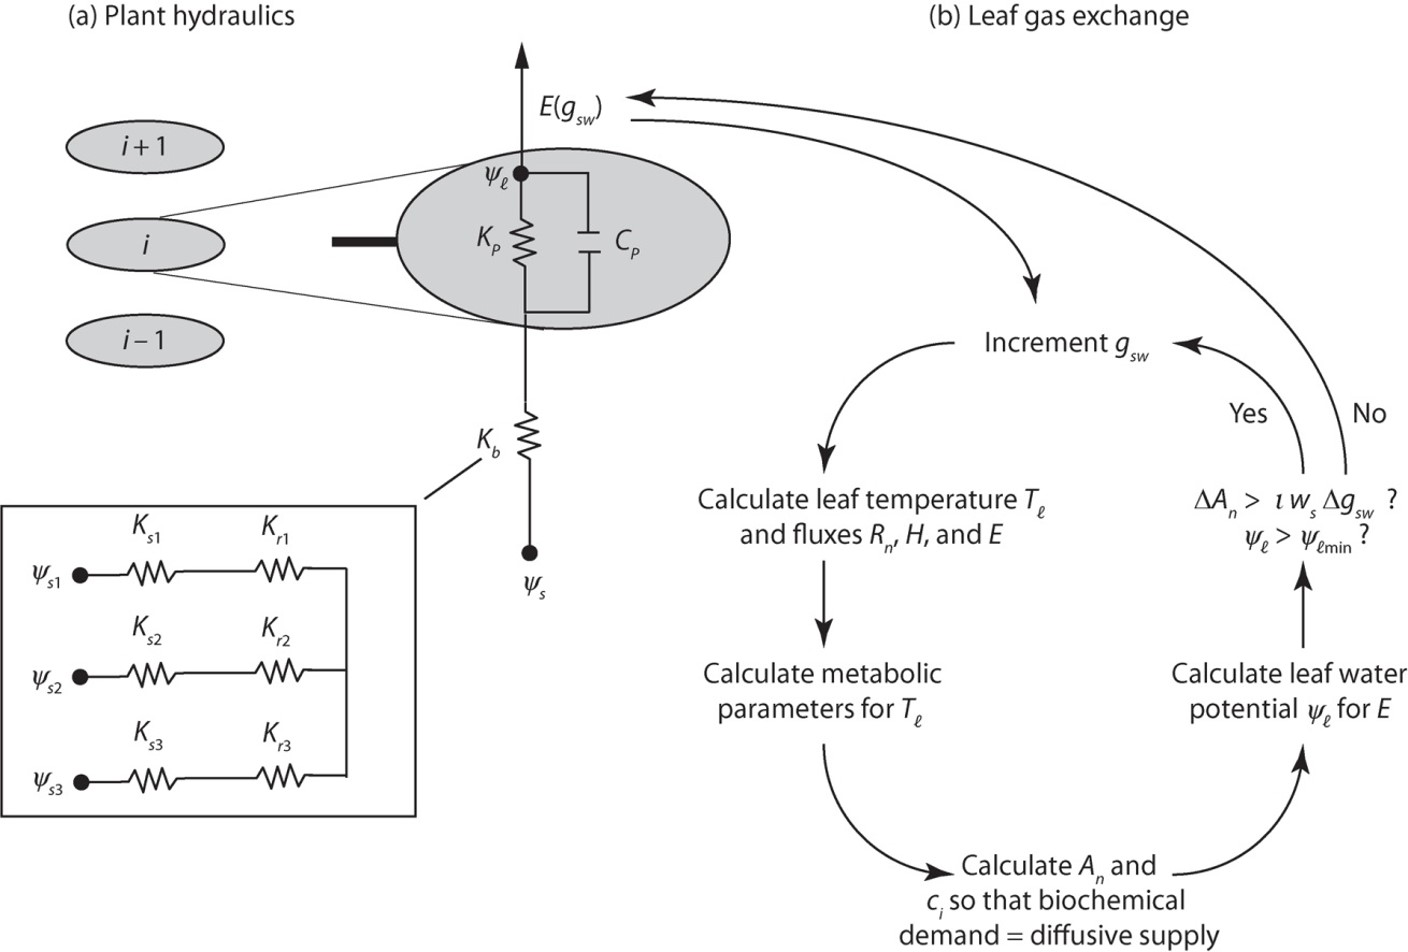
\includegraphics[width=0.8\linewidth]{figures/chap2/SPA} 

}

\caption{Depiction of (a) plant hydraulics and (b) leaf gas exchange in the Soil–Plant–Atmosphere (SPA) model. SPA is a multilayer canopy model.(Bonan 2019)}\label{fig:f219}
\end{figure}

Different models give different results (Figure \ref{fig:f220}): full line: Ball-Berry, dashed line: other models. The shapes of the curves are similar, but there is a difference between them.

\begin{figure}

{\centering 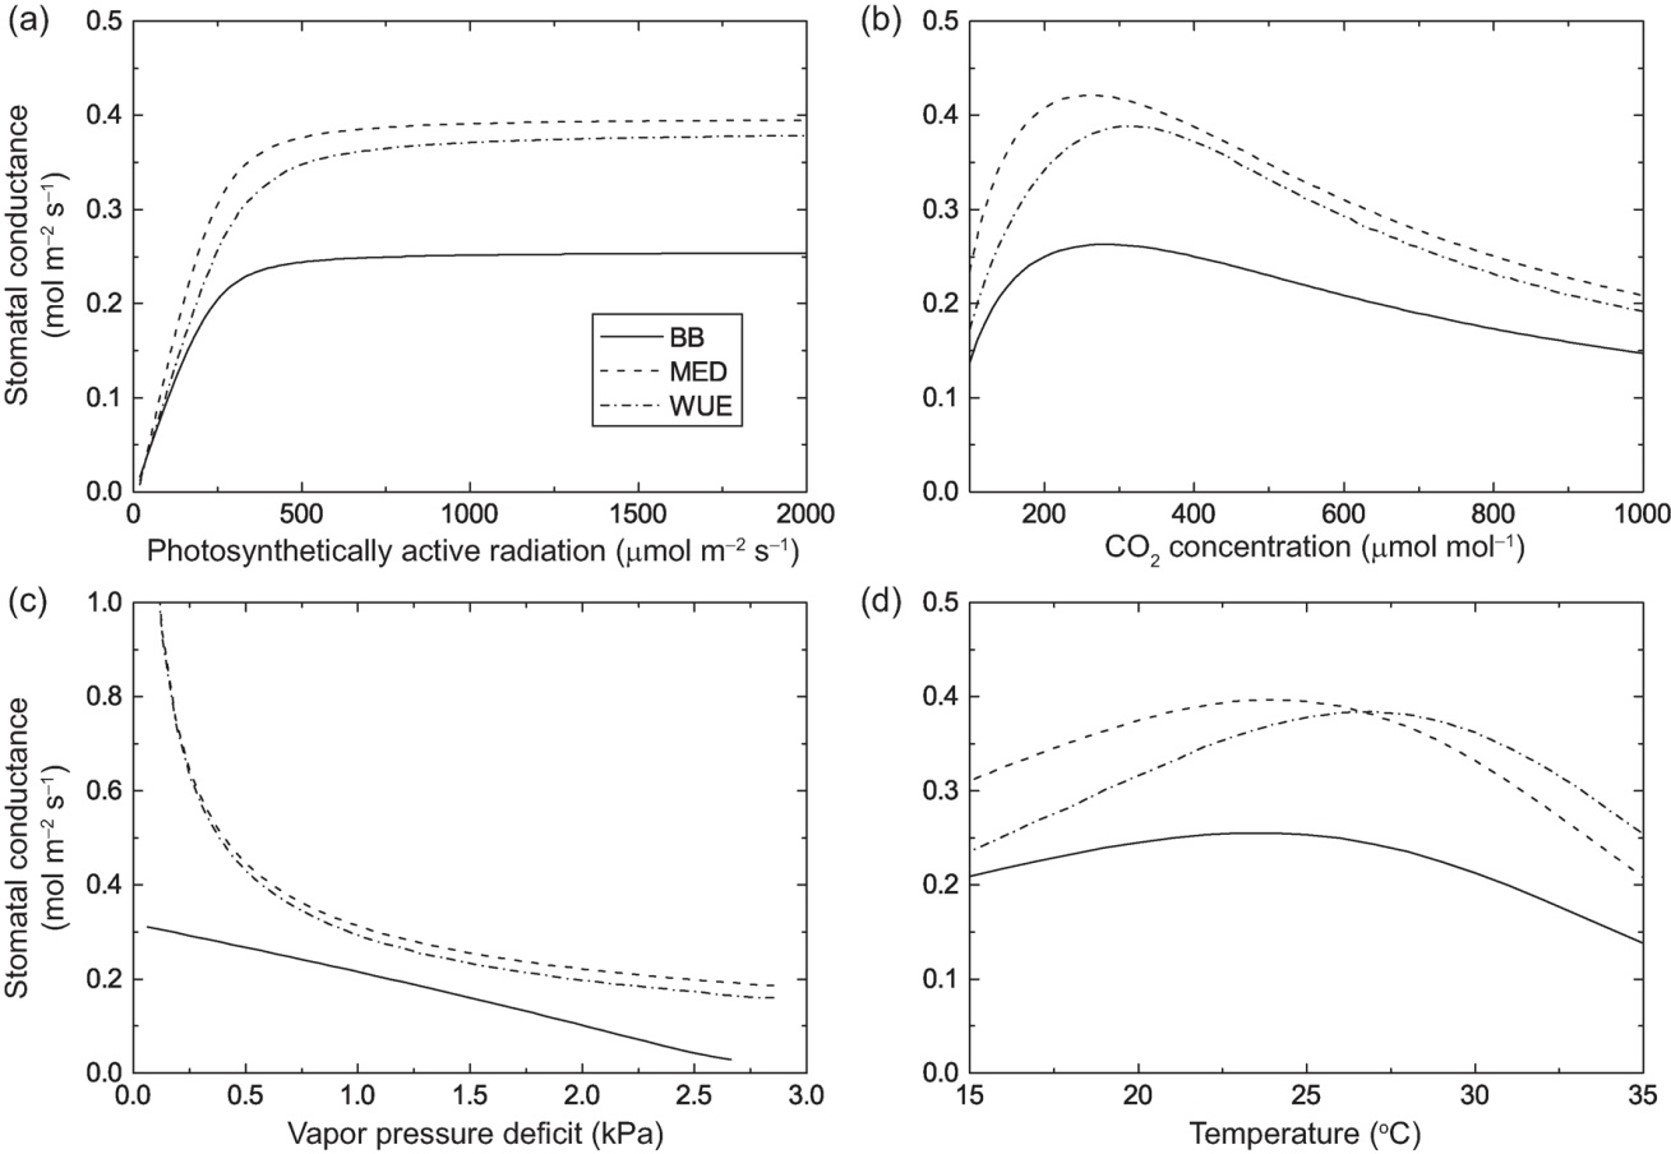
\includegraphics[width=0.8\linewidth]{figures/chap2/modelling_approaches} 

}

\caption{Simulated stomatal responses for various modelling approaches. (Bonan 2019)}\label{fig:f220}
\end{figure}

\hypertarget{upscaling-from-leaf-to-canopy}{%
\section{Upscaling from leaf to canopy}\label{upscaling-from-leaf-to-canopy}}

In this chapter we discussed all processes at the leaf level, but in a forest or other vegetation type, every leaf is different. E.g. the difference between sun and shade leaves.

Figure \ref{fig:f221}: different responses for shade and sun leaves: big differences!
on the long term there is also genetic adaptation to the environmental conditions they are living in.

\begin{figure}

{\centering 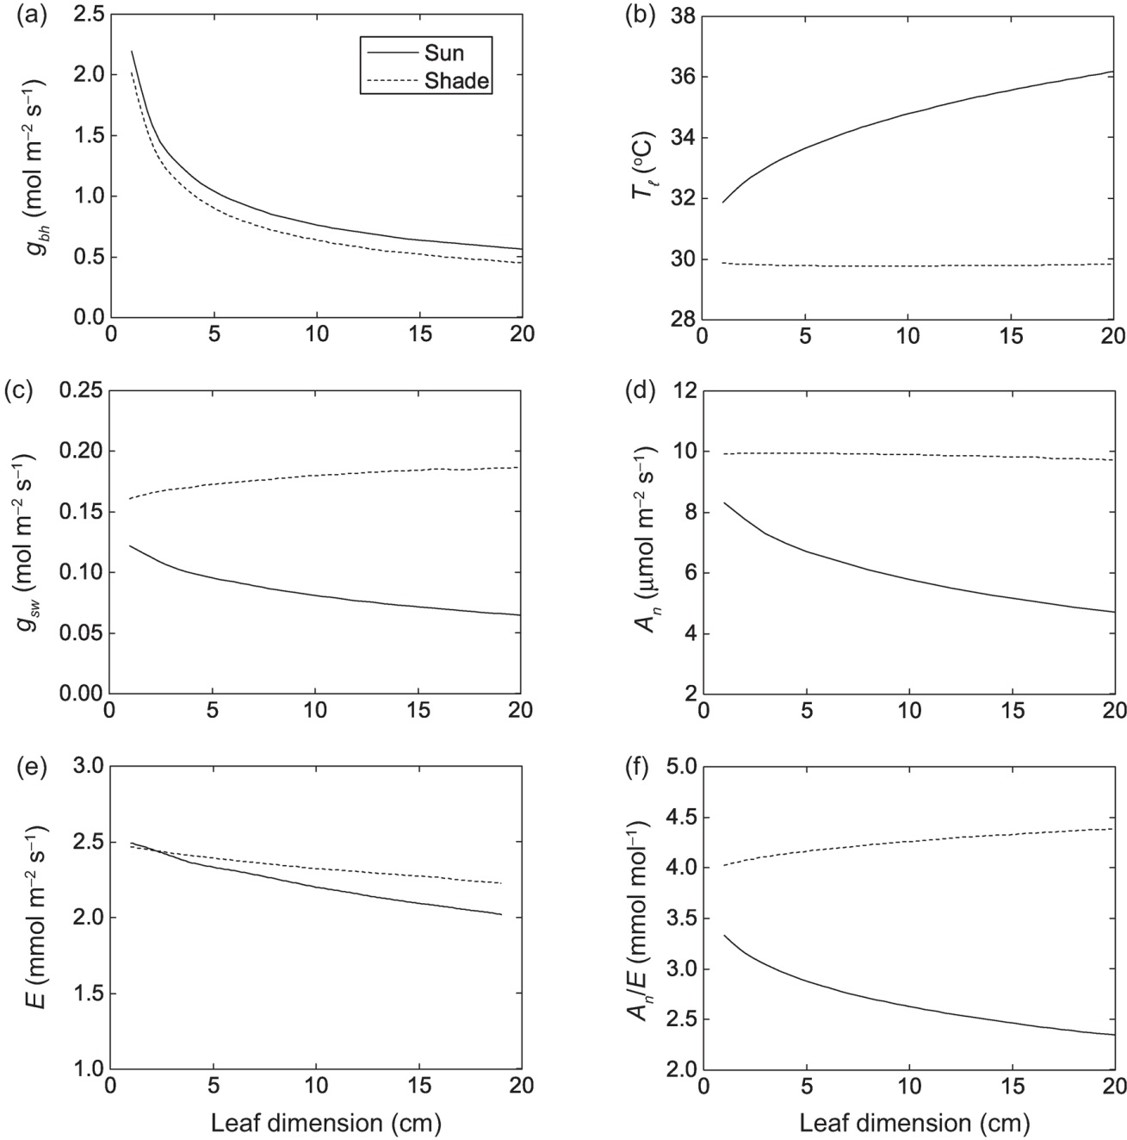
\includegraphics[width=0.8\linewidth]{figures/chap2/sun_shade} 

}

\caption{Leaf microclimate and boundary layer processes in relation to leaf dimension for sun and shade conditions.(Bonan 2019)}\label{fig:f221}
\end{figure}

If you calculated GPP (Figure \ref{fig:f222}), you need to take into account that leaves are not the same all over the world -\textgreater{} see coming lectues.

\begin{figure}

{\centering 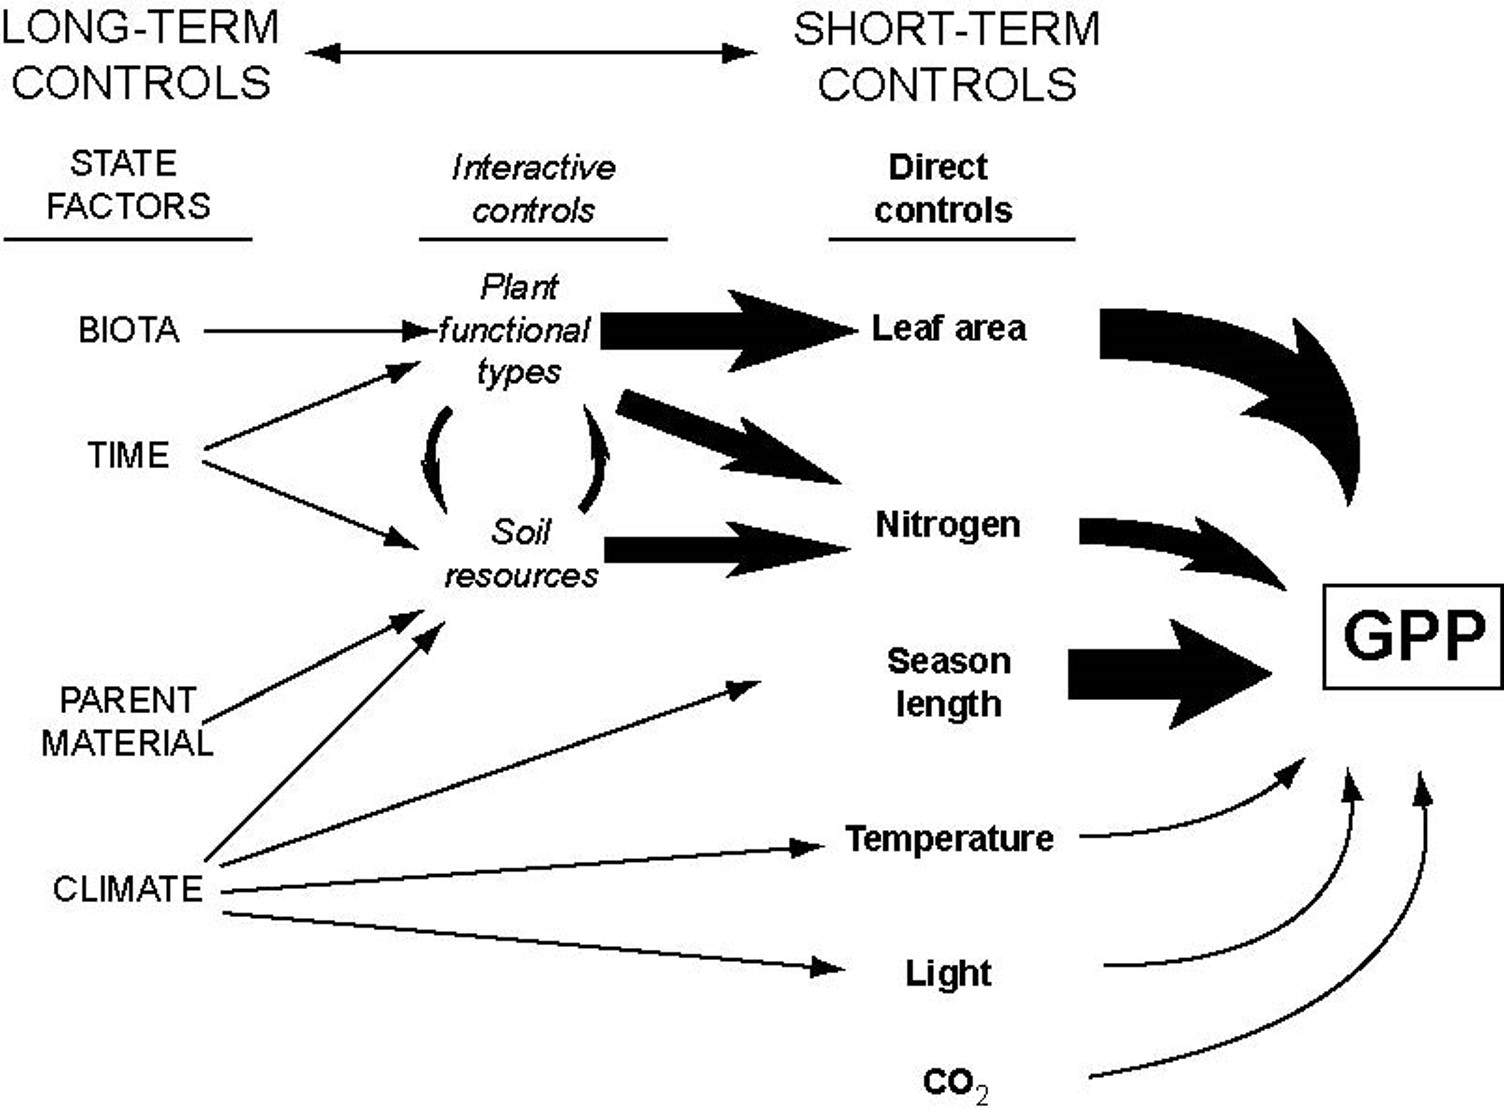
\includegraphics[width=0.8\linewidth]{figures/chap2/GPPcontrols} 

}

\caption{Controlling facors on ecosystem GPP. (Chapin)}\label{fig:f222}
\end{figure}

Thicker arrow means a stronger influence on ecosystem long term GPP.

\hypertarget{case-studies}{%
\section{Case studies}\label{case-studies}}

\hypertarget{case-study-2.1-ozone-impact-on-global-gpp}{%
\subsection{Case study 2.1 Ozone impact on global GPP}\label{case-study-2.1-ozone-impact-on-global-gpp}}

\textbf{Sitch et al.~2003: Indirect radiative forcing of climate change through ozone effects on the land-carbon sink}

The evolution of the Earth's climate during the 21th century depends on the rate at which \(CO_2\) emissions are removed by the ocean and land carbon cycles . To asses/simulate this removal, climate-carbon cycle models are used, but these typically neglect the impacts of changing atmospheric chemistry (e.g.~\(CO_2\) and ozone concentration). Ozone causes cellular damage inside leaves that adversely affects plant production and reduces photosynthesis. In this case study, a global land carbon cycle model - modified to include the effect of ozone and to account for interactions between ozone and \(CO_2\) - is used to estimate the impact of projected changes in ozone levels on the land-carbon sink.

Large scale model. It used a similar leaf gas exchange model as discussed above, but they added an extra equation that reduces stomatal conductance depending on the ozone concentrations (higher ozone levels reduce photosynthesis). The impact of the ozone is highest in tropical zones, with reductions up to 30\%, which will impact the \(CO_2\) storage of tropical forests.

\begin{figure}

{\centering 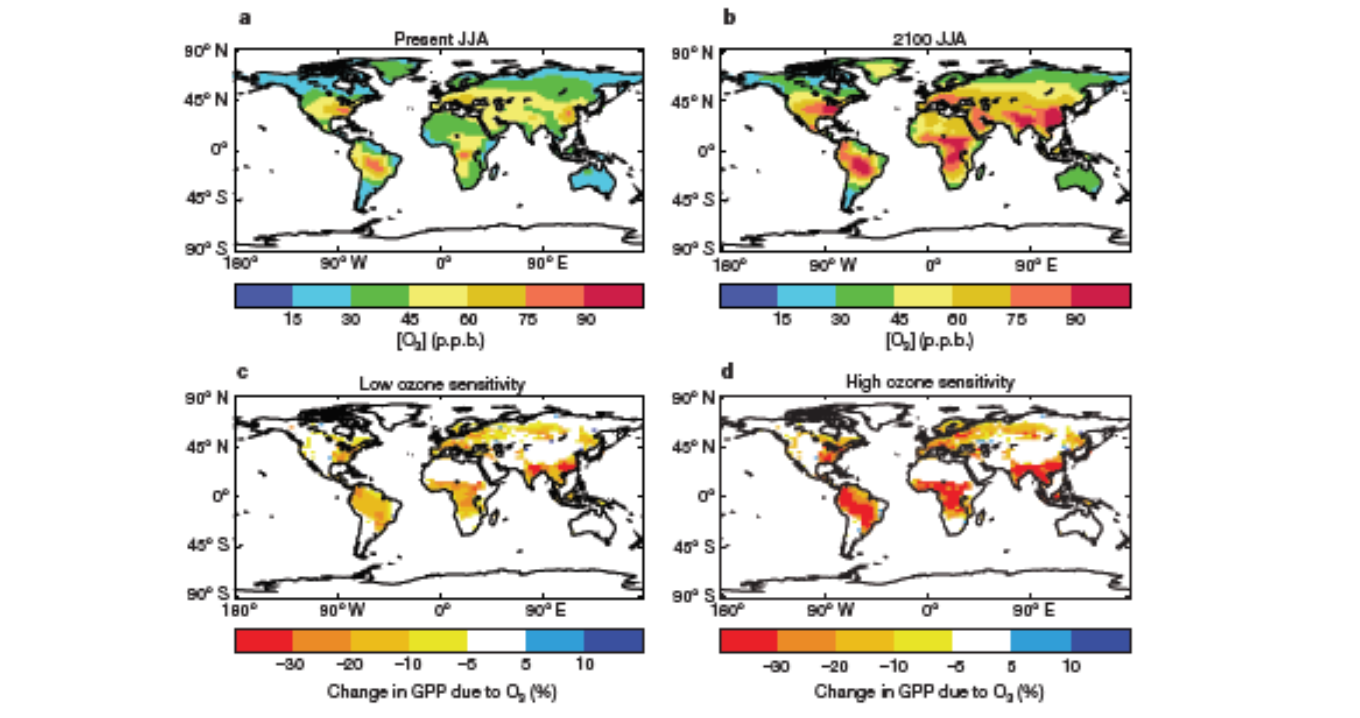
\includegraphics[width=0.8\linewidth]{figures/chap2/ozone} 

}

\caption{Simulated global GPP reduction in response to current and future atmospheric ozone concentrations}\label{fig:f223}
\end{figure}

\hypertarget{case-study-2.2-drought-impact-on-rainforest-gpp}{%
\subsection{Case study 2.2 Drought impact on rainforest GPP}\label{case-study-2.2-drought-impact-on-rainforest-gpp}}

\textbf{Fisher et al.~2007: The response of an Eastern Amazonian rain forest to drought stress: results and modelling analyses from a througfall exclusion experiment }

Climate change projections predict harsher droughts in the Amazon rain forest which could change the amount of \(CO_2\) the forest can absorb, creating a positive feedback system. A lack in appropriate data and process-level understanding creates uncertainty in predicting the forest gas exchange as a response too drought. In this paper these two problems are addressed: new and better data is collected with a TFE experiment and a model (SPA) that predicts sap-flow with soil moisture data is created and fitted to the TFE data. This model is then validated with other independent data.

\begin{figure}

{\centering 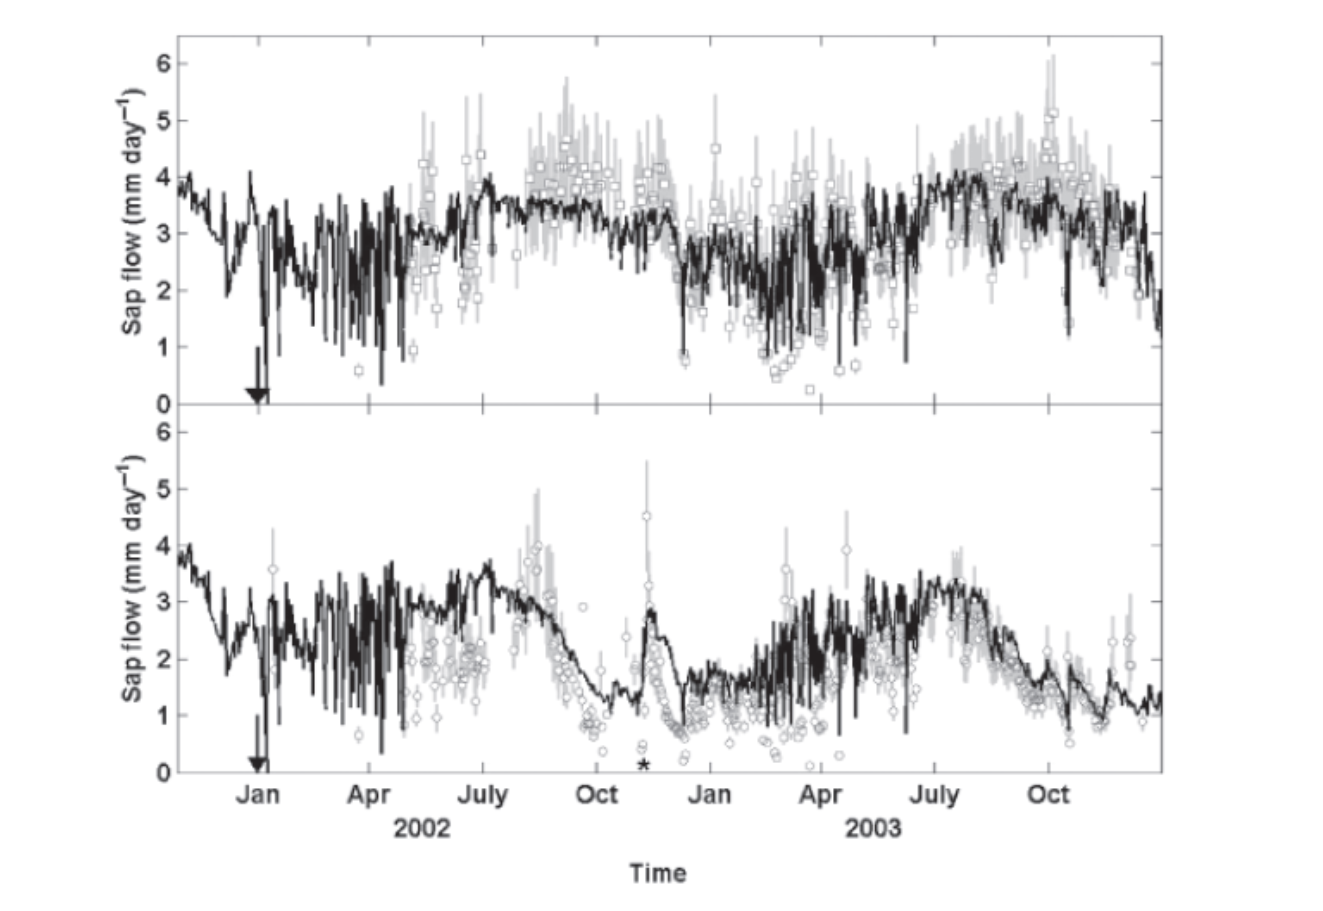
\includegraphics[width=0.8\linewidth]{figures/chap2/fisher1} 

}

\caption{Simulated (SPA model) and observed sapflow for a drought experiment in the Amazon; Fisher et al. 2007}\label{fig:f224}
\end{figure}

Figure \ref{fig:f225} shows the simulations og gs and GPP, black: control plot, grey: dry plot.

\begin{figure}

{\centering 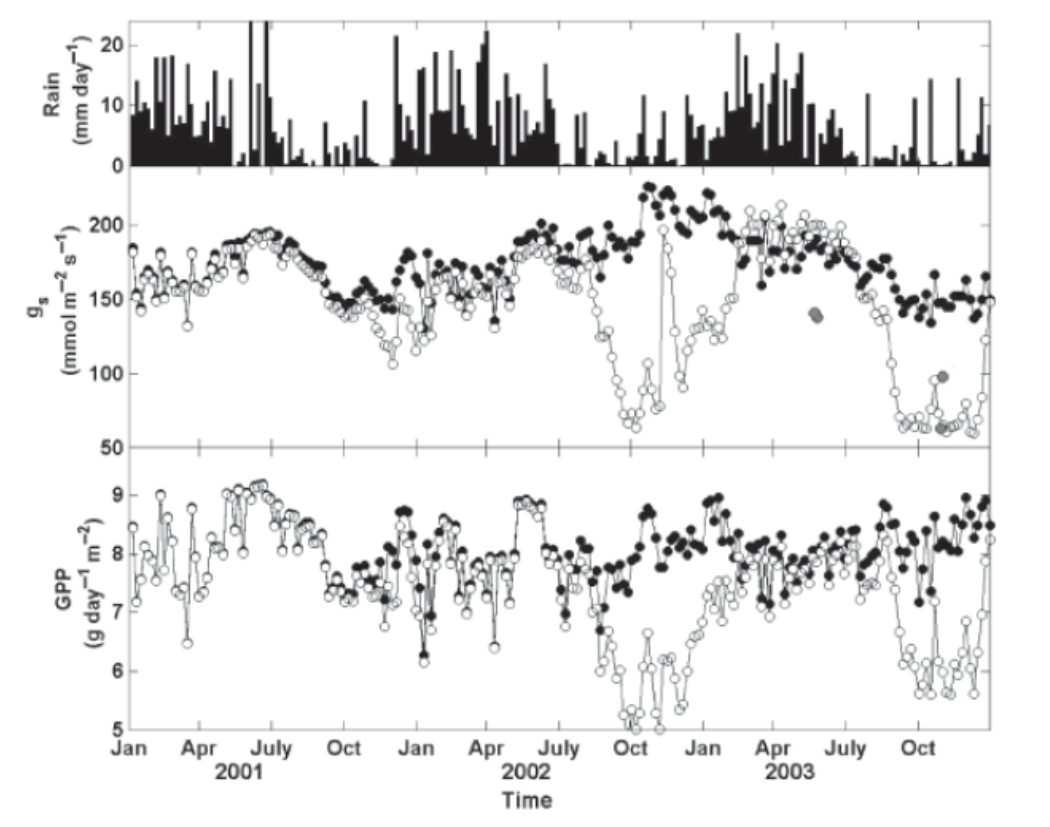
\includegraphics[width=0.8\linewidth]{figures/chap2/fisher2} 

}

\caption{Simulated (SPA model) gs and GPP for a drought experiment in the Amazon. Fisher et al. 2007}\label{fig:f225}
\end{figure}

Conclusions: this model worked better than empirical models, which really predict a collapse of the system. This model is doing better because it simulates the water transport through the tree.
Models need to take into account deep rooting, trees do have access to water in the deep soil, even in the dry period.

\hypertarget{modelling-radiation-vegetation-canopies-and-energy-balance}{%
\chapter{Modelling radiation, vegetation canopies, and energy balance}\label{modelling-radiation-vegetation-canopies-and-energy-balance}}

\chaptermark{Light}

\hypertarget{introduction}{%
\section{Introduction}\label{introduction}}

This chapter deals with upscaling processes from leaf level to canopy level, but still on a (very) short timescale (\textasciitilde hours, sub-daily).

We want a model that is consistent over different scales. If we measure parameters at the leaf level and put those parameter values in our model, we want the results to be as consistent as possible with the data at the canopy scale, for example data from eddy covariance flux towers. Also the other way around, if we optimize model parameters based on flux tower measurements, we want the resulting leaf parameters to be as close as possible to the parameters observed in the field at leaf level.

We first refresh some basics on radiation. The sun emits shortwave radiation, the earth emits longwave radiation (invisible). Longwave radiation has its maximum intensity at a much longer wavelength and contains a much lower amount of energy (surface under the spectral intensity curve). The spectrum of wavelengths the sun emits is different when we measure it on the earth surface (compared to the spectrum at the top of the atmosphere, as the atmosphere absorbs some of the radiation, e.g.~in the ultraviolet light and infrared light absorption takes place. Diffuse radiation (which indirectly reaches the surface) is more shifted towards the blue light, which is one of the wavelengths used by plants. On a sunny day, both diffuse and direct radiation reach the plants. Under full cloud cover, plants only receive diffuse radiation. 50\% of the shortwave radiation is PAR (Photosynthetic Active radiation). PAR is typically expressed as a photon flux density (micromols of photons per m² per s). The lower the zenith angle (higher sun), the higher the PAR fraction in the diffuse and direct radiation that reaches the earth surface. The relative PAR fraction is higher in diffuse radiation.

Secondly, we need to refresh some basics on canopy structure parameters. The leaf area index (LAI) is the total leaf area per unit of ground area. Sometimes it is also defined as the total double-sided surface of the leaves (so the two sides of the leaf), but this is not commonly used. The projected leaf area depends on the orientation of the leaf. Vertically oriented leaves have a smaller projected leaf area than if they would be horizontally oriented. Figure \ref{fig:f31} shows a generalized example of the leaf area density distribution for different vegetation types. The peak of leaf area density is different depending on the vegetation type, with a peak higher in the vegetation for forests and more in the middle for grass. The total LAI is calculated by integrating the function \(a(z)\) showed in figure \ref{fig:f31} over the height. If you keep in mind that trees are higher than grass, it is clear that the total LAI will be bigger for trees than for grass.

\[
total \, LAI = \int_0^{h_c}a(z) \cdot dz
\]

\begin{figure}

{\centering 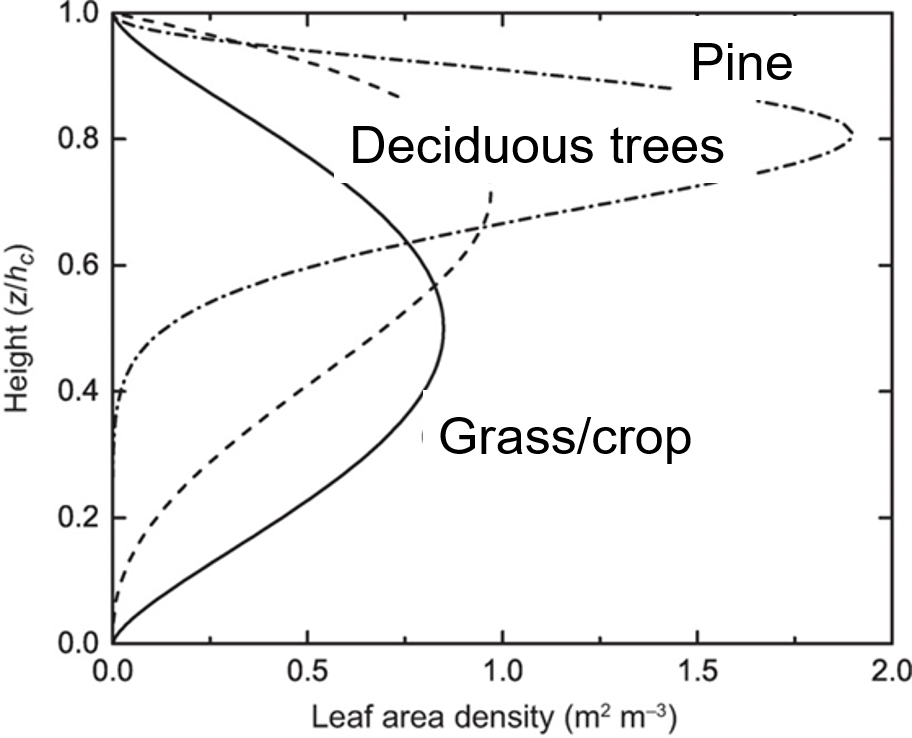
\includegraphics[width=0.8\linewidth]{figures/chap3/f31_LAD} 

}

\caption{Generalized profiles of leaf area density in plant canopies. (Bonan)}\label{fig:f31}
\end{figure}

The cumulative LAI represented in Figure \ref{fig:f32} shows the LAI above a certain point in the canopy. It is calculated as the integral of the function between that point and the canopy height. This figure also shows the cumulative wood area index. If we make the sum of the LAI and the wood area index (WAI) we get the plant area index PAI, which is the total area of plant material per unit of ground area.

\[
cumulative \, LAI = \int_z^{h_c}a(z) \cdot dz
\]

\begin{figure}

{\centering 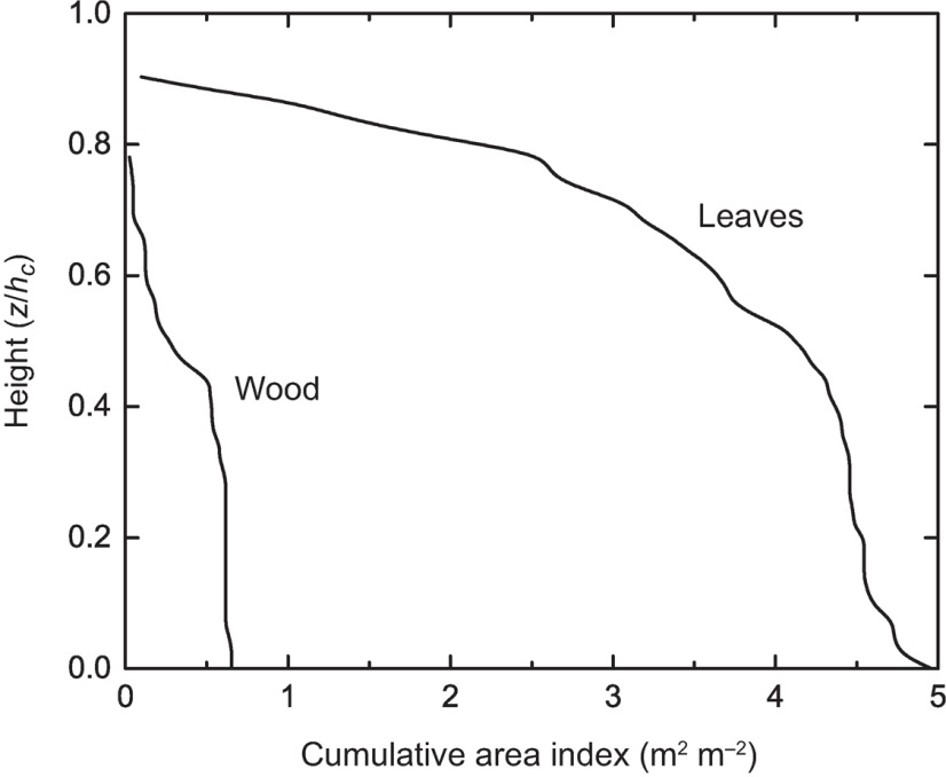
\includegraphics[width=0.8\linewidth]{figures/chap3/f32_cLAI} 

}

\caption{Cumulative LAI and WAI in a deciduous oak-hickory forest. (Bonan)}\label{fig:f32}
\end{figure}

The leaf angle (distribution) is a key structural property of a vegetation canopy. It will largely determine how light will penetrate in the canopy, and is important for other processes, like precipitation interception. Figure \ref{fig:f33} illustrates that the leaf angle can be expressed as the angle between the leaf and the horizontal plane, or as the angle between the zenith line and the line perpendicular to the leaf surface.

\begin{figure}

{\centering 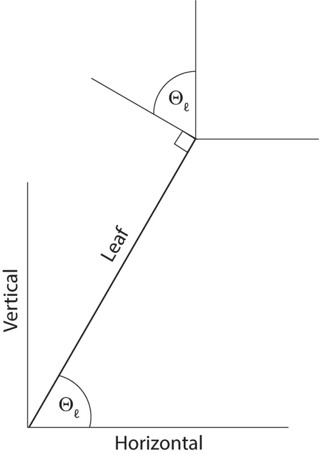
\includegraphics[width=0.8\linewidth]{figures/chap3/f33_Langle} 

}

\caption{Illustration of a leaf (thick line) oriented at an angle Θℓ to horizontal. (Bonan)}\label{fig:f33}
\end{figure}

Leaf angle distributions describe a probability density function of leaf angles of a plant or vegetation. Base on these distribution we can distinguish differences between plants and vegetation types. Planophile leaf angle distributions: most leaves are horizontally oriented; erectophile: most leaves are vertically oriented; plagiophile: average leaf inclination angle is 45°; spherical: mostly used in modelling, corresponds somehow to erectophile, it is a kind of idealized form. This distributions are illustrated in Fig. \ref{fig:f34} Subplot b indicates the cumulative distribution of the leaves.

\begin{figure}

{\centering 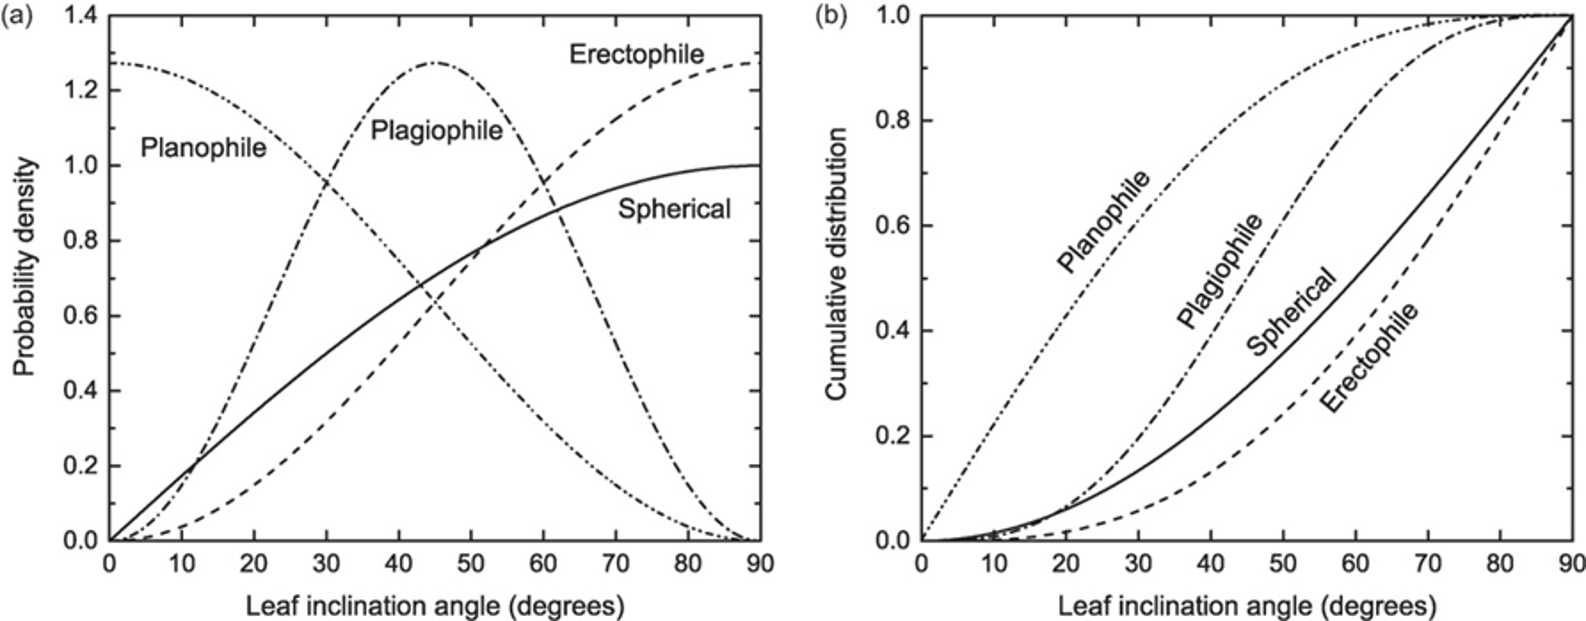
\includegraphics[width=0.8\linewidth]{figures/chap3/f34_angle_distr} 

}

\caption{Planophile, erectophile, plagiophile, and spherical leaf angle distributions showing (a) the probability density function f(Θℓ) and (b) the cumulative distribution F(Θℓ). (Bonan)}\label{fig:f34}
\end{figure}

Figure \ref{fig:f35} illustrates the impact of leaf orientation in two crops on light penetration in the canopy of two crops (lower panel). The complexity of the vegetation plays an important role in where the light is intercepted and how much is intercepted (upper panel). In an erectophile leaf orientation, the light interception is more evenly spread through the vegetation than for a planophile profile, where most of the interception takes place at the center of the vegetation.

\begin{figure}

{\centering 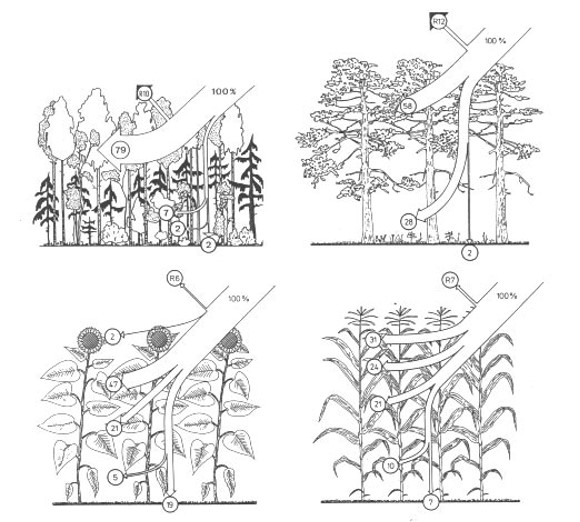
\includegraphics[width=0.8\linewidth]{figures/chap3/f35_architecture} 

}

\caption{Illustration of leaf angle distributions and canopy architecture in general influences radiation attenuation in vegetation canopies.}\label{fig:f35}
\end{figure}

Light extinction follows a typical exponential course when it is observed at multiple heights in vegetation, it decreases very fast at the top of the canopy, with almost no light reaching the soil in this example (Fig. \ref{fig:f36}).
We can conclude that radiative transfer in the canopy depends on:

\begin{itemize}
\tightlist
\item
  the LAI (amount of leaves),
\item
  the optical properties (which depend on the morphology and chemical composition) of the leaves
\item
  the organization of the leaves (architecture, angles,..)
\end{itemize}

\begin{figure}

{\centering 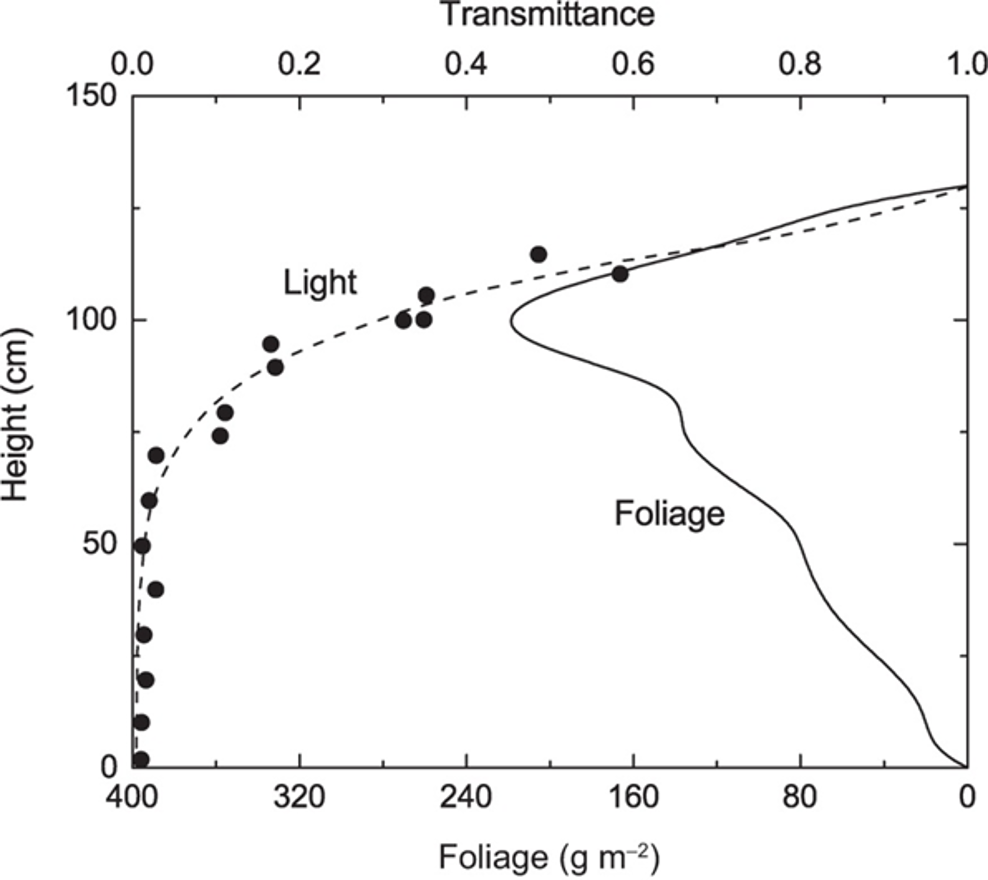
\includegraphics[width=0.8\linewidth]{figures/chap3/f36_obs_profile} 

}

\caption{Profile of light and foliage in a stand of herbaceous plants approximately 130 cm tall. The horizontal axis shows transmittance as a fraction of incident radiation (top axis) and foliage mass (bottom axis) at various heights in the canopy. (Bonan)}\label{fig:f36}
\end{figure}

Radiative transfer theory aims to integrate the light environment of individual vegetation elements (leaves, branches, \ldots) over the entire canopy. It must distinguish between the specific behavior of direct beam radiation and omnidirectional diffuse radiation and it should account for wavelength.

\hypertarget{radiative-transfer-modelling}{%
\section{Radiative transfer modelling}\label{radiative-transfer-modelling}}

Radiative transfer modelling in full 3D is very complex and is a separate branch of science. The radiative transfer schemes in vegetation models are usually relatively simple approximations of full 3D radiative transfer. Such schemes have a lot of assumptions: all leaves are plane-parallel oriented, leaf layers are horizontally homogeneous. We mostly use a one dimensional representation of the canopy (Fig.\ref{fig:f37}), which is often used in vegetation models. Such an approach neglects the horizontal heterogeneity of vegetation and only assume a simplified vertical heterogeneity. A more complex model, subplot b, represents a three dimensional representation of the canopy, with vertical and horizontal variation.

\begin{figure}

{\centering 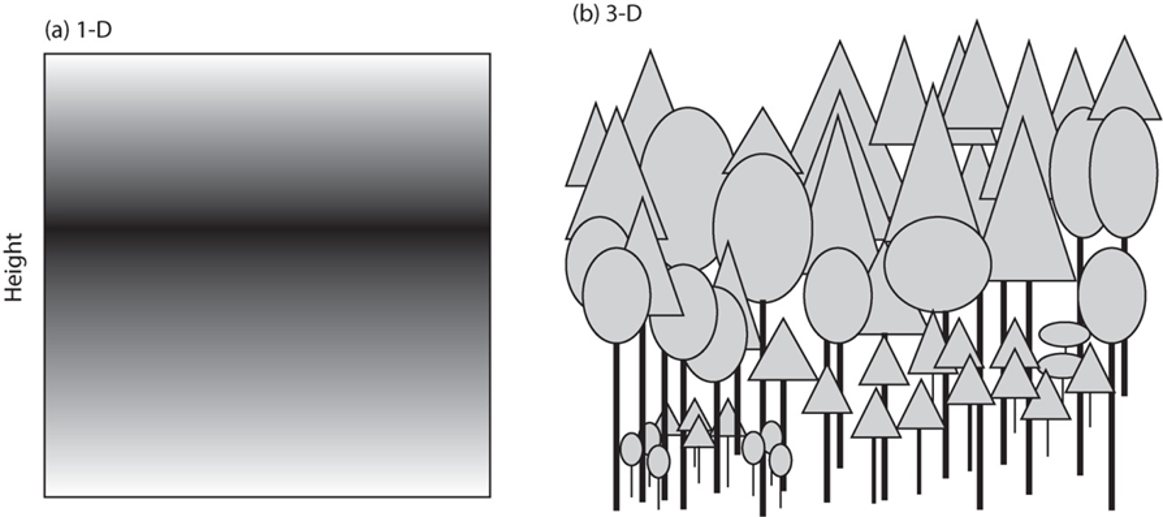
\includegraphics[width=0.8\linewidth]{figures/chap3/f37_RT_principle} 

}

\caption{Representation of a canopy as (a) one-dimensional with a vertical profile of leaf area (shown by grayscale gradation in which darker shading denotes more leaves) that is horizontally homogenous and (b) threedimensional with vertical and spatial structure determined by crown geometry and spacing. (Bonan)}\label{fig:f37}
\end{figure}

\hypertarget{leaf-optical-properties}{%
\subsection{Leaf optical properties}\label{leaf-optical-properties}}

What happens to light when it reaches a leaf? It can be absorbed, reflected or transmitted. We express these in relative fractions as \(\rho\) = reflectance (albedo), \(\tau\) = transmittance, \(\alpha\) = absorbance. Leaves absorb PAR, with a small negative peak at the green light, which they reflect more compared to blue and red light. Also in the infrared wavelength band, radiation is absorbed (mostly longwave radiation). UV light is absorbed by the cuticula to protect the leaves. The reflectance and transmittance curves are inverse curves from the absorptance curve. Here, infrared radiation and green light are reflected/transmitted. The clear difference between VIS and NIR is used in remote sensing for vegetation indices (e.g.~NDVI). Transmittance depends on the thickness of the leave.

\begin{figure}

{\centering 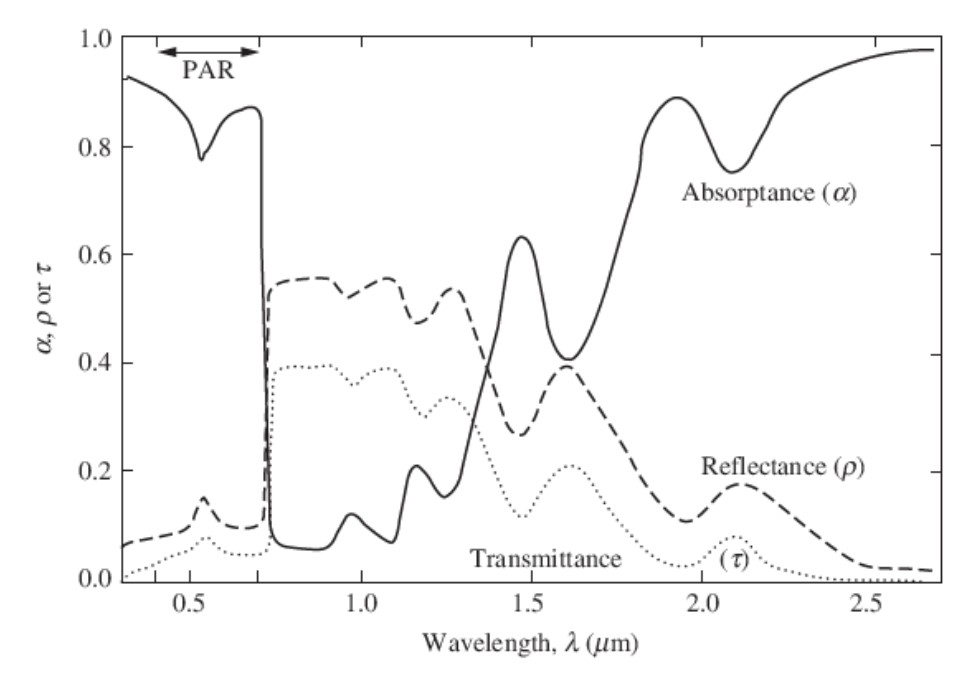
\includegraphics[width=0.8\linewidth]{figures/chap3/f37_leaf_optical} 

}

\caption{Spectrum of absorptance, reflectance and transmittance of a typical plant leaf (Jones, 2014)}\label{fig:f37b}
\end{figure}

The albedo of the total canopy is typically lower than that of its individual leaves, as light that is transmitted or reflected by one leave can be absorbed by another leaf (multiple scattering) (see Table below). Reflectance of needles is lower than the reflectance of broadleaves.

\begin{center}
\captionof{table}{Table showing typical reflectance and absorptance values for leaves and vegetation canopies of different Plant Functional Types (PFT).(Jones, 2014)}
\label{table:reflectance}

\begin{center}\includegraphics[width=0.8\linewidth]{figures/chap3/f38_table_optical} \end{center}
\end{center}

\hypertarget{light-transmission-without-scattering}{%
\subsection{Light transmission without scattering}\label{light-transmission-without-scattering}}

The most basic radiative transfer models, do not consider scattering (no reflection on the leaf). The Beer-Bouguer-Lambert law describes the attenuation of light through a homogeneous medium with thickness \(dz\) in absence of scattering. The absorbed radiation is proportional to the thickness of the medium, the amount of light that comes in and a constant \(K\).

\[
dI^{\downarrow} = -KI^\downarrow dz
\]

with \(dz\): thickness; \(I^\downarrow\): incoming radiation; \(K\): constant; \(dI^\downarrow\): absorbed radiation in the medium.

After integration we can calculate the radiation \(I\) leaving the medium from \(I_0\), the radiation intensity entering the medium.

\[
I^{\downarrow} = I^{\downarrow}_0\cdot e^{-Kz}
\]

For leaves in a canopy, and based on probability theory, Monsi and Saeki (1953) applied the Beer law for a volume with crown thickness \(dz\), with randomly distributed horizontal elements (leaves) with density \(N\) (number of elements per volume, see Fig. \ref{fig:f39}.

\[
dI^{\downarrow} = - I^{\downarrow} a N dz
\]

where the total leaf area in the volume can be calculated as:

\[
L = aNz
\]

with \(N\): density of leaf elements; \(L\): total leaf area; \(a\): surface of individual leaf perpendicular to the path of light; \(z\) the total thickness of the canopy.

After integration we get an exponential function that describes the radiation extinction in the canopy:

\[
I^{\downarrow} = I^{\downarrow}_0\cdot e^{-L}
\]

\begin{figure}

{\centering \includegraphics[width=0.8\linewidth]{figures/chap3/f39_beer} 

}

\caption{Transmission of solar radiation through a homogeneous medium in the absence of scattering. In this example, n non-overlapping opaque particles each with cross-sectional area a oriented perpendicular to the path of light are placed in a medium with cross-sectional area A and thickness dz. The radiation absorbed in the medium is dI.(Bonan)}\label{fig:f39}
\end{figure}

However, in real canopies not all leaves are horizontal, and the light is not coming in perpendicular as assumed in the original equation of Monsi and Saeki. In the exponential function, \(L\) should therefore be adapted to the projected leaf area perpendicular to the light beams, as the model assumes that light comes in perpendicularly.

\[
I^{\downarrow} = I^{\downarrow}_{sky,b}\cdot e^{-K_bL}
\]

Where \(K_b\): direct beam extinction coefficient, and \(LH\) (horizontal leaf area)= \(K_b L\). And \(I^{\downarrow}_{sky,b}\) is the incident radiation at the top of the canopy. \(K_b\) describes how severe light is attenuated in the canopy depending on the LAI. A higher \(K_b\) indicates a faster extinction, so a more dark forest. Fig. \ref{fig:f310} describes the light transmittance with increasing LAI for different \(K_b\) values.

\begin{figure}

{\centering \includegraphics[width=0.8\linewidth]{figures/chap3/f310_Kb} 

}

\caption{Transmission of direct beam radiation τb in relation to leaf area index for typical values of the extinction coefficient Kb. (Bonan)}\label{fig:f310}
\end{figure}

The extinction coefficient depends on solar zenith angle and leaf orientation (as illustrated in Fig.\ref{fig:f311}).

\[
K_b = \frac{L_H}{L} = \frac{G(Z)}{cosZ}
\]

With \(Z\): solar angle; \(\Theta_l\): leaf angle; \(G(Z)\): function depending on the zenith angle (shown in figure \ref{fig:f311}). Divided by \(cosZ\) because we project to the horizontal plane. \(L_h\): leaf area projected on the horizontal plane.

\begin{figure}

{\centering \includegraphics[width=0.8\linewidth]{figures/chap3/f311_LLh} 

}

\caption{Extinction coefficient in relation to solar zenith angle Ζ and leaf inclination angle. In each panel, a unit leaf area (L = 1), shown with a thick line, is projected onto a horizontal surface $L_H$ so that $K_b = L_H$. The leaf inclination angle is 0° (bottom panels), 30° (middle panels), and 60° (top panels). In the left and middle columns, the leaf is oriented towards the Sun and the solar zenith angle is 0° (left column) and 15° (middle column). In the right column, Ζ = 15°, but the leaf is oriented away from the Sun. In each panel, the arrows indicate the solar beam (Bonan)}\label{fig:f311}
\end{figure}

The lower the sun is to the horizon (the higher the zenith angle), the higher the extinction coefficient is, except for horizontal leaves, which have a constant \(K_b\) of 1.

\begin{figure}

{\centering \includegraphics[width=0.8\linewidth]{figures/chap3/f312_Kb_angle} 

}

\caption{Extinction coefficients for horizontal, spherical, and vertical leaf angle distributions. (a) Direct beam radiation Kb in relation to solar zenith angle. (b) Diffuse radiation Kd in relation to leaf area index(Bonan)}\label{fig:f312}
\end{figure}

The above described formulas do not only allow us to describe the light extinction in the canopy, but also to calculate the sun and shaded fraction of leaf are in the canopy. If we divide the canopy into multiple layers, we can calculate for each layer which part is in the sun and which part is in the shade. For every canopy layer, the fraction of sunlit leaves is equal to the fsun(x) function. It represents the amount of light that comes through the layers above it.

\[
f_{sun} (x) = e^{-K_b x}
\]

Where \(x\) is the cumulative LAI above the layer of interest. Similarly we can calculate the actual sunlit leaf area within a certain layer:

\[
\Delta L_{sun} = \frac{e^{-K_b x} \left(1 - e^{-K_b \Delta L} \right)}{K_b}
\]

Where \(\Delta L\) is the actual amount of leaves in that layer, this formula calculates the difference between the sunlit fraction at the top of the layer minus the ``reduction of sunlit fraction'' within the layer. If we apply that formula on a full canopy we can calculate the sunlit leaf area of the full canopy \(L_{sun}\):

\[
L_{sun} = \frac{\left(1 - e^{-K_b L} \right)}{K_b}
\]

\(L_{sun}\): integrated over the whole canopy. Based on this equation you can calculated the amount of leaves that is sunlit in the canopy. And also the shade fraction based on the difference with the total LAI.

In the example below (Fig. \ref{fig:f313}) the sunlit and total LAI are compared between a vegetation with horizontal and with vertical foliage. The latter has more sunlit leaves, as top leaves don't shade the underlaying leaves. In the horizontal foliage, more light is absorbed, so less light is transmitted than in the vertical foliage.

\begin{figure}

{\centering \includegraphics[width=0.8\linewidth]{figures/chap3/f313_sun_shade} 

}

\caption{Radiative transfer and sunlit leaf area index for a canopy of horizontal leaves (top panels) with Kb = 1 and vertical leaves (bottom panels) with Kb = 0.112. The left-hand panels show a canopy consisting of four layers of leaves. Each thick black line represents a leaf area index of 0.1 m2 m–2. The thin lines depict interception or transmission of beam radiation with a zenith angle of 10°. The middle panels show cumulative leaf area index and sunlit leaf area index with depth in the canopy. The right-hand panels show direct beam transmittance with depth in the canopy. (Bonan)}\label{fig:f313}
\end{figure}

When we study the sunlit LAI with increasing cumulative LAI (Fig.\ref{fig:f314}) for different leaf orientations, the same course of the curve applies: first, there is a linear increase of the amount sunlit leave are index with increasing LAI, after which a saturation occurs when the vegetation becomes more dense (higher LAI). The level of saturation depends on the leaf angle distribution.

\begin{figure}

{\centering \includegraphics[width=0.8\linewidth]{figures/chap3/f314_sunlit} 

}

\caption{Sunlit leaf area index in relation to total leaf area index for horizontal, spherical, and vertical foliage orientations with solar zenith angle Ζ = 30°. Kb = 1, 0.577, and 0.368 for horizontal, spherical, and vertical foliage. (Bonan)}\label{fig:f314}
\end{figure}

A final complicating factor that we want to highlight here is that leaves and canopies are not distributed randomly in space, but occur clumped. Leaf clumping means that leaves appear in groups and that there are larger gaps in between. Clumping can occur at different scales: at leaf level, canopy level or landscape level (Fig.\ref{fig:f315}). The clumping factor (\(\Omega\)) adjusts the amount of light that goes through the vegetation (more light passes through). The factor is added in the radiation extinction equations to adjust the extinction coefficient. Where a clumping factor of 1 represents randomly distributed leaves, while values lower then 1 represent clumped leaves (e.g.~0.74 for needleleaf evergreen forest).

\[
I^{\downarrow} = I^{\downarrow}_{sky,b}\cdot e^{-K_b \Omega L}
\]

\[
f_{sun} (x) = e^{-K_b \Omega x}
\]

\begin{figure}

{\centering \includegraphics[width=0.8\linewidth]{figures/chap3/f315_clumping} 

}

\caption{Images illustrating leaf/canopy clumping a various scales: leaf, crown, stand.}\label{fig:f315}
\end{figure}

\hypertarget{diffuse-transmittance}{%
\subsection{Diffuse transmittance}\label{diffuse-transmittance}}

Diffuse radiation is omnidirectional, and therefore it penetrates better into the canopy. The formula below represents the diffuse transmittance. The last part of the equation represents the contribution of a certain sky angle to the total sky irradiation (e.g.~contribution of zenith angle between Z1 and Z2 in Fig.\ref{fig:f316}). The exponential curve with the leaf area \(L\) is the light extinction curve, but here it is also integrated over the zenith angle.

\[
\tau_d = \frac{I^{\downarrow}}{I^{\downarrow}_{sky,d}} \int_0^{\pi/2} exp\left[- \frac{G(Z)}{cosZ}L \right] sinZcosZdz
\]

\begin{figure}

{\centering \includegraphics[width=0.8\linewidth]{figures/chap3/f316_diffuse} 

}

\caption{Illustration of direct beam and diffuse radiation. The sky forms a bowl, or inverted hemisphere, over a horizontal surface. Shown is a cross section of the sky hemisphere. Direct beam (solid line) originates from the  direction of the Sun with zenith angle Ζ. Diffuse radiation (dashed lines) can be treated as independent beams of radiation each with an angle Ζ. The shaded region is the relative contribution between sky angles Ζ1 and Ζ2 to total sky irradiance.(Bonan)}\label{fig:f316}
\end{figure}

The more leaves, the less diffuse light is transmitted through the canopy. The contribution of the zenith angles is shown on Fig.\ref{fig:f317}. There is more light transmitted in the 30°-60° zenith angle range than in the other two groups. Thus perpendicular diffuse sunlight penetrates less easy in the canopy than sunlight under a 30°-60° angle.

\begin{figure}

{\centering \includegraphics[width=0.8\linewidth]{figures/chap3/f317_diff_trans} 

}

\caption{Transmittance of diffuse radiation τd in relation to leaf area index for a spherical leaf distribution. Show are the transmittances for sky zones of 0°–30°, 30°–60°, and 60°–90° and also the total transmittance. Fill patterns show the contribution of each sky zone to total transmittance.(Bonan)}\label{fig:f317}
\end{figure}

It is also interesting to compare the diffuse transmission to the direct transmission. The dashed line (Fig.\ref{fig:f318}) indicates the transmittance for diffuse light (omnidirectional), the solid lines indicate the transmittance for direct light at different solar zenith angles. The transmittance of diffuse light is higher than that of direct light for solar zenith angles greater than 40-50°, direct light penetrates less easy through the canopy compared to diffuse light.

It is important to include diffuse radiation into models as it penetrates deeper into the canopy, it is shifted towards the blue light, which is used by plants for photosynthesis, and because plants depend on it in cloudy conditions.

\begin{figure}

{\centering \includegraphics[width=0.8\linewidth]{figures/chap3/f318_diff_dir_trans} 

}

\caption{Transmission of solar radiation through a canopy with spherical leaf distribution in relation to leaf area index. The solid lines show direct beam transmittance τb for solar zenith angles of 0°–80° (in 10° increments).The dashed line shows the diffuse transmittance τd. (Bonan)}\label{fig:f318}
\end{figure}

\hypertarget{the-norman-model1979}{%
\subsection{The Norman Model(1979)}\label{the-norman-model1979}}

In the Norman model, the canopy is divided into multiple layers of typically 0.5 LAI per layer. For each layer the diffuse, direct and longwave radiation balance is calculated: reflection, absorption and transmission. The model thus accounts for scattering. We do not discuss the equations in detail, but the large number of equations have to be solved numerically, which is very computational expensive, especially in model versions where a sunlit and shade fraction per leaf layer are considered.

\begin{figure}

{\centering \includegraphics[width=0.8\linewidth]{figures/chap3/f319_Norman} 

}

\caption{Radiative fluxes in a canopy of N leaf layers. The vertical profile is oriented with i = 1 the leaf layer at the bottom of the canopy, leaf layer i + 1 above layer i, and i = N the leaf layer at the top of the canopy. Each layer has a leaf area index ΔL. is the downward diffuse shortwave flux onto layer i, is the upward diffuse shortwave flux above layer i, and is the unscattered direct beam flux onto layer i. and are the corresponding downward and upward fluxes of longwave radiation. These depend on leaf Tℓand ground Tg temperatures. Thick arrows denote boundary conditions of diffuse solar radiation , direct beam solar radiation, and atmospheric longwave radiation at the top of the canopy.(Bonan)}\label{fig:f319}
\end{figure}

\hypertarget{the-goudriaan-and-van-laar-model-1994}{%
\subsection{The Goudriaan and van Laar Model (1994)}\label{the-goudriaan-and-van-laar-model-1994}}

This is an analytical solution of the model, which integrates over a single calculation step. To be able to do so, one integrated extinction coefficient for all layers is assumed (K'b, adapted extinction coefficient). One light extinction coefficient is thus used for diffuse and direct radiation together, which is the major simplification in the model. This coefficient also includes a clumping factor. This model is widely used due to its simplicity and low computational demand. It can be applied to a single layer or multi-layer canopy. Due to its assumptions, this model produces more errors, especially for diffuse light (under cloudy conditions).

\begin{figure}

{\centering \includegraphics[width=0.8\linewidth]{figures/chap3/f320_goudriaan} 

}

\caption{ Derivation of absorbed direct beam solar radiation for a leaf layer with leaf area index ΔL (Goudriaan 1982). $ρ_c$ is the reflectance of the leaf layer.(Bonan)}\label{fig:f320}
\end{figure}

\hypertarget{the-two-stream-approximation}{%
\subsection{The Two-Stream approximation}\label{the-two-stream-approximation}}

This model takes ``the best of both worlds''. It is called ``two stream''" because it calculates light penetration separately for direct and diffuse radiation, but it has an analytical solution. It can be used for multilayer models.

\begin{figure}

{\centering \includegraphics[width=0.8\linewidth]{figures/chap3/f321_two_stream} 

}

\caption{Fluxes for (a) direct beam and (b) diffuse radiation in the twostream approximation for a canopy with leaf area index L.(Bonan)}\label{fig:f321}
\end{figure}

The three approaches (Norman/Goudriaan/two stream) are all based on the same theory. They are implemented in a different way, but the results are very similar for direct light. However they show substantial deviations for diffuse light, shaded leaves and denser canopies.

\hypertarget{longwave-radiation}{%
\subsection{Longwave radiation}\label{longwave-radiation}}

Longwave radiation is important for closing the energy balance. To simulate longwave radiation transfer in canopies, similar approaches as above are used, but the emission of longwave radiation by the ground, and leaf surfaces need to be accounted for.

\begin{figure}

{\centering \includegraphics[width=0.8\linewidth]{figures/chap3/f322_LW} 

}

\caption{Longwave radiation fluxes represented for a single leaf layer.(a) Norman’s (1979) numerical model. Shown is the radiative balance for leaf layer i + 1 located above leaf layer i. (b) A simplified model to allow only forward scattering and to permit an analytical solution integrated over a canopy. In both panels, emitted radiation is excluded. Thick lines denote fluxes incident onto the layer. (Bonan)}\label{fig:f322}
\end{figure}

\hypertarget{representing-canopy-structure-in-models}{%
\section{Representing canopy structure in models}\label{representing-canopy-structure-in-models}}

\hypertarget{big-leaf-models}{%
\subsection{Big-leaf models}\label{big-leaf-models}}

Big leaf models can have a shaded and a sunlit fraction in the canopy, or can consider sunlit leaves only. The forest/vegetation is represented as one big leaf, with a leaf area equal to the total leaf area of the forest/vegetation. Such models do not account for the vertical structure of the canopy. These models calculate properties of the big leaf, by upscaling. For example by caluculating an average stomatal or caopy conductance. Evapotranspiration can then be calculated by applying the Penman-Monteith equation and a canopy level conductance. The leaf boundary layer is replaced by the atmosphere surface layer and gsw is the average stomatal conductance of the whole forest.

\begin{figure}

{\centering \includegraphics[width=0.8\linewidth]{figures/chap3/f323_bigleaf} 

}

\caption{Scaling of leaf fluxes to the canopy using a big-leaf model. (a) Shown are leaf sensible heat, transpiration, and CO2 fluxes in relation to various conductances. Fluxes are exchanged between the leaf and air around the leaf. Also shown is the total resistance. (b) Shown are big-leaf canopy fluxes in which leaf fluxes are scaled by the average conductance and leaf area index and are further modified by turbulent transport in the atmospheric surface layer. Surface layer processes are commonly omitted for CO2 exchange. Only a single big leaf is shown, but separate sunlit and shaded big leaves can be similarly depicted. (Bonan)}\label{fig:f323}
\end{figure}

It is not an easy task to integrate GPP (e.g.~calculated by the Farquhar model of Chapter 2) over a canopy represented by a big leaf. We cannot just give the total light absorbed by the canopy to a photosynthesis model, as we need to account for the non-linearity in the process. The task is easier if Amax is assumed to decrease exponentially together with light availability I the canopy, which is a reasonable assumption, as we know that leaf nitrogen content is decreasing from the top to the bottom of the canopy. As such we are assuming a ``photosynthesis extinction''" instead of a light extinction in the canopy.

\[
GPP = \int_0^LA(x)dx
\]

\[
A_{max}(x) = A_{max0}e^{-K_bx}
\]

\[
GPP = \int_0^{L}A(x)dx = A(0) \left[\frac{1 - e^{-K_b L}}{K_b} \right]
\]

However, this is a rough approach, and it does not account for the nonlinear canopy responses. A better approach is to include a sunlit and shade fraction of the leaves. Where the GPP is calculated as the sum for sunlit and shaded leaves separately. Each fraction has a separate value for \(g_s\), \(A_m\) etc\ldots{}

\[
GPP = \left[A_{sun} f_{sun} + A_{shade} (1 - f_{sun}) \right]L
\]

Big leaf models that use the Fraquhar approach often assume an integrated Vcmax value for the canopy, calculated based on an exponential profile of \(V_{cmax}\).

\[
V_{cmax}(x) = V_{cmax0} e^{-K_n x}
\]

\begin{figure}

{\centering \includegraphics[width=0.8\linewidth]{figures/chap3/f324_vcamx_profile} 

}

\caption{Canopy profiles of relative photosynthetic capacity in relation to cumulative leaf area index. Thin lines show exponential profiles using values of Kn for 16 temperate broadleaf forests and two tropical forests ranging from 0.10 to 0.43 (Lloyd et al. 2010). The two thick lines show observed profiles of Vcmax and Jmax from Niinemets and Tenhunen (1997) obtained for sugar maple (Acer saccharum). (Bonan)}\label{fig:f324}
\end{figure}

\hypertarget{multilayer-models}{%
\subsection{Multilayer models}\label{multilayer-models}}

Account for al vertical heterogeneity, such as light, leaf physiology, leaf traits and even micrometeorology, e.g.~RH is different at different leaf layers in the model. All equations (fluxes, energy balance) are calculated for each layer, and GPP is the sum of the photosynthesis of all layers. Figure \ref{fig:f325}: each layer is a big leaf to calculate all leaf level processes. Radiative transfer and leaf fluxes are thus simulated for each layer. Sometimes, even leaf hydraulics are simulated, to simulate leaf water potential and its influence on stomatal conductance. Such models are computationally expensive, especially because they is solved for each layer a set of equations in an iterative way (Fig. \ref{fig:f326}). Nevertheless, such multilayer models are very common in large scale land surface models. Be aware that horizontal heterogeneity is not considered in these models, see later chapters for that.

\begin{figure}

{\centering \includegraphics[width=0.8\linewidth]{figures/chap3/f325_multilayer_process} 

}

\caption{Overview of the main processes in a multilayer canopy model.The canopy is represented by N leaf layers with layer i + 1 above layer i. (a) Diffuse and direct beam solar radiation is transmitted or intercepted. The intercepted portion is absorbed or scattered in the forward and backward direction. Longwave radiation is similar to diffuse radiation. (b) Leaf sensible heat, transpiration, and CO2 fluxes depend on absorbed radiation and leaf boundary layer and stomatal conductances. Sensible heat is exchanged from both sides of the leaf. Water vapor and CO2 can be exchanged from one or both sides of the leaf depending on stomata. Leaf temperature is the temperature that balances the energy budget. (c) Stomatal conductance depends on leaf water potential. Plant water uptake for a canopy layer is in relation to belowground soil and root conductance and aboveground stem conductance acting in series and also a capacitance term. (d) Scalar profiles are calculated from a conductance network. Leaf fluxes provide the source or sink of heat, water vapor, and CO2, along with soil fluxes. (e) Sensible heat, latent heat, and heat storage in soil depend on the ground temperature that balances the soil energy budget. (f) The wetted fraction of the canopy layer depends on the portion of precipitation that is intercepted. (Bonan)}\label{fig:f325}
\end{figure}

\begin{figure}

{\centering \includegraphics[width=0.8\linewidth]{figures/chap3/f326_multilayer_solving} 

}

\caption{Flow diagram of processes in a multilayer canopy model. The shaded area denotes leaf processes resolved at each layer in the canopy. This is a generalized diagram of the required calculations for a dry leaf. Specific models differ in how the equation set is solved and the iterative calculations. Evaporation of intercepted water requires additional complexity.(Bonan)}\label{fig:f326}
\end{figure}

\hypertarget{d-ray-tracing-models}{%
\subsection{3D ray tracing models}\label{d-ray-tracing-models}}

3D ray tracing models are not (yet) use as part of operational vegetation models. They rather for a separate group of models, focus on radiative transfer only (they do not simulate other processes such as photosynthesis). These models are typically used to simulate what a satellite (or other remote sensing sensor) would observe in specific wavelength bands. As such these models are very useful for interpretation of remote sensing observations. They really simulate how light, or individual sun rays penetrate the canopy and do that for the different wavelengths. Based on such models we can also get better insight in radiative transfer and derive better radiative transfer schemes for operational vegetation models.

\begin{figure}

{\centering \includegraphics[width=0.8\linewidth]{figures/chap3/f327_DART} 

}

\caption{Example of the PROSPECT leaf optical model and the DART 3D ray tracing model.}\label{fig:f327}
\end{figure}

These models typically consider simple 3D objects with specific optical properties. However, the newest addition to this research is using detailed 3D reconstructions of trees from lidar scans as model input and run the model with the lidar data as scattering objects in the 3D scene.

\begin{figure}

{\centering \includegraphics[width=0.8\linewidth]{figures/chap3/f328_TLS_RT} 

}

\caption{Example of a study that uses terrestrial laser scanning (TLS) to construct a full 3D model of a forest as input for a 3D ray tracing model (Kükenbrink et al. 2020) }\label{fig:f328}
\end{figure}

\hypertarget{ecosystem-energy-balance}{%
\section{Ecosystem energy balance}\label{ecosystem-energy-balance}}

\hypertarget{basic-principles}{%
\subsection{Basic principles}\label{basic-principles}}

The energy balance is a fundamental part of vegetation models. The goal is to calculate how much energy comes in, how much is lost and in what the resulting temperature is for the leaf or the surface. The energy balance is governed by non-linear equations. However linearizations exist (e.g.~Penman Monteith equations to calculate ET).

\hypertarget{surface-radiation-balance}{%
\subsection{Surface radiation balance}\label{surface-radiation-balance}}

The formula below (Fig. \ref{fig:f329}) calculates the radiation balance

\begin{figure}

{\centering \includegraphics[width=0.8\linewidth]{figures/chap3/f329_rad_balance} 

}

\caption{Radiative balance of an opaque gray body receiving downwelling solar S and longwave L radiation.(Bonan)}\label{fig:f329}
\end{figure}

where \(R_n\): net radiation (how much energy is available for system), \(\rho S^{\downarrow}\): reflected shortwave radiation, \(\epsilon \sigma T^{4}\) the Stefann-Boltzman law. The equation essentially makes the balance between how much shortwave net comes in, and how much longwave is net reflected. The net radiation forms the major input term of the energy balance.

\hypertarget{bulk-surface-energy-balance}{%
\subsection{Bulk surface energy balance}\label{bulk-surface-energy-balance}}

This is the central equation of the surface energy balance:

\[
R_n = \lambda E + H + G +S
\]

The net radiation is the input of energy to the ecosystem which is dissipated via multiple loss terms: latent heat (evapotranspiration), sensible heat flux, ground heat flux and energy storage (in the biomass of the ecosystem). Most of the energy goes to the latent heat to well-watered active vegetation (e.g.~a beach forest in summer).

It is really important to close the energy balance in models. All factors in the equation can be formulated in terms of input factors of the model, such as incoming radiation, and in function of the surface temperature. The equation below is rewriting the above equation in terms of surface temperature.

\[
\sum_{\Lambda} (1 - \rho_{\Lambda} ) S^{\downarrow}_{\Lambda} + \epsilon L^{\downarrow} = Q_{a} \\ = \epsilon \sigma \theta_s^{4} + c_p ( \theta_s - \theta_{ref} ) g_{ac} + \frac{\lambda \left[ q_{sat} ( \theta_s ) - q_{ref} \right] }{ g_c^{-1} + g_{ac}^{-1}} + \frac{k}{\Delta z} (\theta_s - T_1)
\]

Where \(S\) input energy (shortwave) in a certain wave length band (\(\Lambda\)), \(Q\) is the total gross incoming energy. At the right side of the equation we see: the longwave loss term, sensible heat loss, latent heat (in response to vapor pressure) , and the ground heat flux. The surface temperature (\(\Theta_s\)) is the big leaf surface temperature.

The big leaf latent heat (evapotranspiration), in often accounted by the Penman-Monteith equations (as function of net radiation and vapor pressure deficit).

\[
\lambda E = \frac{s (R_n - G) + c_p \left(q_{sat}(T_a) - q_a \right) g_{ac}}{s + (1 + \frac{g_{ac}}{g_c}) \frac{c_p}{\lambda}}
\]

\begin{figure}

{\centering \includegraphics[width=0.8\linewidth]{figures/chap3/f330_E_balance} 

}

\caption{Conductance networks for sensible heat flux (top) and latent heat flux (bottom) for various depictions of the land surface. This chapter describes the bulk surface and big-leaf canopies. (Bonan)}\label{fig:f330}
\end{figure}

\hypertarget{leaf-energy-balance}{%
\subsection{Leaf energy balance}\label{leaf-energy-balance}}

Some models make the leaf energy balance, which is essentially using the same equations as the bulk energy balance, but applying them at the leaf (layer) level and solving team for leaf temperature. The leaf energy balance depends on radiative forcing, boundary layer processes and stomatal physiology. The stomatal conductance is balance photosynthesis, transpiration and energy fluxes.

\[
c_L \frac{\delta T_l}{\delta t} = Q_a - 2 \epsilon_l T_l^4 - H(T_l) + \lambda E(T_l)
\]

\[
Q_a = \sum_\Lambda S^{\downarrow}_\Lambda (1 + \rho_{g \Lambda})(1 - \rho_{g \Lambda} - \tau_{l \Lambda}) + \epsilon_l (L_{sky}^\downarrow+ L_g^{\uparrow})
\]

The dimension of the leaf plays an important role in the solving of the leaf energy balance, for example, the boundary layer conductance depends on the leaf dimensions and the wind speed.

\begin{figure}

{\centering \includegraphics[width=0.8\linewidth]{figures/chap3/f331_leaf_E_balance} 

}

\caption{Biophysics and biochemistry of leaves. (a) The radiative environment consists of solar radiation (left) and longwave radiation (right). (b) Leaf fluxes include CO2, H2O, and heat through the boundary layer. These fluxes are shown as a network of conductances for the adaxial (upper) and abaxial (lower) leaf surfaces. For H2O and CO2, the conductance for each surface is obtained from stomatal and boundary layer conductances acting in series. The total conductance is defined by the adaxial and abaxial surfaces acting in parallel. (c) Stomata open to absorb CO2 for photosynthesis, but, in doing so, water is lost as transpiration. (Bonan)}\label{fig:f331}
\end{figure}

\hypertarget{case-studies-1}{%
\section{Case studies}\label{case-studies-1}}

\hypertarget{case-study-3.1}{%
\subsection{Case study 3.1}\label{case-study-3.1}}

How is the amount of diffuse light impacting photosynthesis? (diffuse radiation fertilization) In normal circumstances, the sun leaves are in the saturated zone of photosynthesis, while shaded leaves are somewhere on the linear increase part. If you would change the radiation composition (e.g.~more clouds), this would result in less light for the sunlit leaves, which has only limited impact on their photosynthesis. For the shaded leaves on the other hand, more diffuse radiation has a big impact on the photosynthesis. So, the hypothesis in this study is that if you have more diffuse radiation, more photosynthesis takes place at the canopy level. This hypothesis is tested by using data of two fluxtower stations and a multilayer vegetation model.

\begin{figure}

{\centering \includegraphics[width=0.8\linewidth]{figures/chap3/f332_knohl1} 

}

\caption{Principle of the effect of increased diffuse raditaion on leaf/canopy photosynthesis. (Knohl et al. 2008)}\label{fig:f332}
\end{figure}

The x axis (Fig. \ref{fig:f333}) represents the diffuse radiation over the total radiation. Photosynthesis increases with increasing diffuse radiation an reaches a maximum at 45\% diffuse light. Transpiration increases also but at a slower pace, and the water use efficiency increases faster. So, forests have a higher water use efficiency when the amount of diffuse radiation is higher (again with max but now around 0.65). On cloudy days the Rd/Rs is higher than the optimum. The net carbon balance increased if you have more diffuse light (in relative terms), the transpiration remains stable but the WUE is increasing (more photosynthesis for the same amount of transpiration). However, for the studied sites, the situation is in 61\% of the time beyond the optimum (on cloudy days), resulting in a net decreasing impact on the net carbon uptake.

\begin{figure}

{\centering \includegraphics[width=0.8\linewidth]{figures/chap3/f333_knohl2} 

}

\caption{Resulting impact of changing diffuse fraction on carbon and water fluxes and WUE (Knohl et al. 2008)}\label{fig:f333}
\end{figure}

\hypertarget{case-study-3.2}{%
\subsection{Case study 3.2}\label{case-study-3.2}}

Studies have shown that the increase of atmospheric CO2 since the 1850's caused an enhancement in plant growth, but the magnitude varies. This enhancement also manifests itself in the enhancement of LAI (leaf area index), the area of leafs on a specific ground area.
In the paper, Boreal Ecosystem Productivity Simulator (BEPS) was used as process-based diagnostic model. It initially was used, as the name states, for boreal ecosystems, but has been adapted for all ecosystems on Earth. It simulates the impact of drivers (climate, CO2 concentration, and nitrogen deposition) on the GPP (Gross Primary Production) and as well carbon pools below GPP and respiration activities, generally, the whole carbon cycle, this on a daily time interval for each pixel. It makes use of various satellite data (assimilate LAI) and LUE (light-use efficiency) models.

Running these simulations on three LAI series, it stated that the enhancement of LAI contributed 12,4\% to the accumulated carbon sink.
In satellite observations it was observed that the global leaf area index has increased over the past 40 years, and they wanted to investigate whether this has had an effect on global carbon sink. The model used in this study is driven by remote sensing data, it is a diagnostic and not really a process-based model. The model calculates the GPP based on the equation (seen today) which used LAIshade and LAIsun based on similar equation with exponential function, clumping factor and so on. The study aims to quantify how much the LAI increase is contributing to the simulated carbon uptake globally.
Map shows the trends of the LAI in the world.

\begin{figure}

{\centering \includegraphics[width=0.8\linewidth]{figures/chap3/f334_chen1} 

}

\caption{Global map of LAI trend between 1981 and 2016 based on remote sensing (Chen et al. 2021).}\label{fig:f334}
\end{figure}

They calculated the different factors which are accounted for in their model and tested how sensitive their model result was to that different driving factors. According to the model, global ecosystem productivity has increased (light blue line in Fig. \ref{fig:f335}). N deposition did not a net effect. Climate change (T increase, drought stress) has reduced the sink strength. The LAI increase had a positive impact, contributes to the increased sink.
They observed that the relative increase of the maximum LAI per year was larger than the relative increase of the average LAI per year. This indicates that the average LAI increase is mainly caused by the higher maximum LAI, and not by the lengthening of the growing season.

\begin{figure}

{\centering \includegraphics[width=0.8\linewidth]{figures/chap3/f335_chen2} 

}

\caption{Simulated impact of different factors contributing to the increased global land C sink since 1981 (Chen et al. 2021) }\label{fig:f335}
\end{figure}

\hypertarget{modelling-temporal-and-seasonal-dynamics}{%
\chapter{Modelling temporal and seasonal dynamics}\label{modelling-temporal-and-seasonal-dynamics}}

\chaptermark{dynamics}

The main topic of this chapter is temporal variations in fluxes and leaf seasonality. We will study the upscaling in time, going from instantaneous processes to daily and seasonal dynamics (temporal dynamics), focusing on phenology.

\hypertarget{introduction-on-temporal-dynamics}{%
\section{Introduction on temporal dynamics}\label{introduction-on-temporal-dynamics}}

An example shows how we use flux data to evaluate the diurnal and seasonal cycles of models (Figure \ref{fig:f41}). The modeled data is shown in black, the measured data in different colors, for different variables. The model can predict diurnal (instantaneous) fluxes good, seasonal cycles are more difficult to predict because the leaf area changes over time.

\begin{figure}

{\centering \includegraphics[width=0.8\linewidth]{figures/chap4/f41_Krinner} 

}

\caption{Evaluation of the temporal dynamics of fluxes (Rn: Net Radiation, H: sensible heat, LE: latent heat, NEE: net ecosystem exchanges of CO2) simulated by the global model ORCHIDEE. LEFT: measured (color) and modelled "summer" diurnal cycle for each flux and each PFT. RIGHT: measured (color) and modelled seasonal cycle for each flux and each PFT. (Krinner et al. 2005)}\label{fig:f41}
\end{figure}

The temporal dynamics of fluxes respond to multiple factors and depending on the scales we are looking at, we need to take other processes into account. If we are interested in \textbf{instantaneous} responses, we need to modulate the physiological processes (stomata of leaves). On the other hand, if we look at \textbf{seasonal} responses, we need to consider both physiology and phenology (the amount of leaves the vegetation has). It is also important to mention \textbf{long-term} responses; for example, if you want to simulate carbon fluxes for the coming decades, more (slower) processes need to be considered (e.g.~forest succession).
The focus of this chapter will be on seasonal responses and phenology. These are processes that are typically calculated on an intermediate time step (e.g.~daily or monthly) in vegetation models.

\hypertarget{phenology-the-background}{%
\section{Phenology: the background}\label{phenology-the-background}}

\textbf{Phenology} is the study of periodic events in biological life cycles and how these are influenced by seasonal and interannual variations in climate, as well as habitat factors (such as elevation). There is a link with carbon allocation, which means how much carbon will be distributed over different plant compartments.
The phenological processes respond to climate variability, the so-called environmental cue, an environmental trigger. For example, from observational data, the ecodormancy responds both to high temperatures and longer day length. It is a complex mechanism with many factors, and we still don't know the underlying physiological processes.

\hypertarget{trends-in-phenology}{%
\subsection{Trends in phenology}\label{trends-in-phenology}}

There are important trends in phenology with climate change because it's not only global average temperatures that are changing, but also spring temperatures are advancing. Autumn temperatures are coming later in the year. Figure \ref{fig:f42} shows an example of needle appearance dates (for larch), where it is possible to identify a trend of needles appearing earlier. New needles of larch trees appear more early over time and this shift is accelerating. Shifts are occurring in the range of weeks. Such phenological trends have an impact on ecosystem functioning, and those impacts of shifting leaf phenology can manifest in multiple ways (Fig. \ref{fig:f43}).

\begin{figure}

{\centering \includegraphics[width=0.8\linewidth]{figures/chap4/f42_Defilia} 

}

\caption{Larch needle appearance in Sargans 1958-2002. Dashed line is trend 1958-1999, solid line is trend 1958-2002.  (Defilia and Clot 2005)}\label{fig:f42}
\end{figure}

\begin{figure}

{\centering \includegraphics[width=0.8\linewidth]{figures/chap4/f43_Polgar} 

}

\caption{Concept of various effect that changing phenology can have on ecosystem processes (e.g. productivity or transpiration). (Polgar and Primack 2011)}\label{fig:f43}
\end{figure}

A shift in phenology has an impact on the functioning of ecosystems. In a normal year the physiological activity (e.g.~photosynthesis) increases after leaves are formed, reaches a maximum, and after the summer a decrease occurs because of less efficient leaves and less light input. Due to changes in phenology, this is influenced (direct or lagged, positive or negative):

\begin{enumerate}
\def\labelenumi{\Alph{enumi})}
\item
  Full positive effect, faster maximum
\item
  A total increase in amount of leaves, also benefits in summer
\item
  Earlier onset of leaves cause earlier senescence of leaves, causing less assimilation in autumn
\item
  Faster ageing leaves: decrease activity after spring
\end{enumerate}

\hypertarget{leaf-phenology-models}{%
\section{Leaf phenology models}\label{leaf-phenology-models}}

Leaf phenology models are essentially models used to update the leaf area state variable for PFTs in vegetation models.

\textbf{Phenology is typically a PFT dependent process in vegetation models:}

\begin{itemize}
\tightlist
\item
  Evergreen PFTs typically have a constant background leaf turnover rate.
\item
  Summer green and rain green PFTs have a leaf phenology driven by environmental factors (temperature, water, light, \ldots).
\end{itemize}

\textbf{How to model phenology?} We don't have (bio)physical models, only empirical models:

\begin{itemize}
\item
  Option 1: prescribed phenology

  \begin{itemize}
  \item
    Prescribed dates of leaf onset and offset (4 dates to determine carbon allocation phases to leaves).
  \item
    Or data assimilation of remote sensing data (LAI).
  \end{itemize}
\item
  Option 2: prognostic phenology

  \begin{itemize}
  \tightlist
  \item
    A complete leaf phenology model includes carbon allocation, leaf onset and growth, and litterfall as influenced by environmental conditions (still empirical).
  \end{itemize}
\end{itemize}

\hypertarget{prescribed-phenology}{%
\subsection{Prescribed phenology}\label{prescribed-phenology}}

An option to model phenology is using the dates of leaf onset and offset (typical 4 dates; start leaf formation, maximal activity, start senescence, all leaves `are gone') .

An alternative is to fit a function to remote sensing data. What is typically done is fitting a logistic function of time to remote sensing observations of leaf phenology:

\[
y(t)=\frac{c}{1+e^{a+bt}}+d
\]

If we observed phenology with satellites, it could be done using vegetation indices (NDVI, EVI, \ldots). Based on observation indices throughout the year, we could define dates to phenological events (Figure \ref{fig:f44})

\begin{figure}

{\centering \includegraphics[width=0.8\linewidth]{figures/chap4/f44_zhang} 

}

\caption{Sample time series of MODIS EVI data and estimate phenological transition dates for a mixed forest pixel in New England. Diamonds: EVI data, solid line with stars: fitted logistic model. (Zhang et al. 2003)}\label{fig:f44}
\end{figure}

This approach allows plotting maps with the key days for phenology (Figure \ref{fig:f45}) and seeing the spacial variance in shifts in phenology. Such datasets can be used to train prognostic models.

\begin{figure}

{\centering \includegraphics[width=0.8\linewidth]{figures/chap4/f45_zhang_map} 

}

\caption{Maps of phenological transition dates for New England. (Zhang et al. 2003)}\label{fig:f45}
\end{figure}

\hypertarget{budburst-models}{%
\subsection{Budburst models}\label{budburst-models}}

Budburst models are prognostic models and are the most developed ones (compared to senescence models for example). They simulate when a bud is becoming a leaf. These models are based on environmental signals (cues), and the most common approaches are:

\begin{itemize}
\tightlist
\item
  Degree day sums (summation of daily temperature above 5°, for example).
\item
  Chilling requirement (to pass the danger of spring frost) (accumulation of cold T).
\item
  Photoperiod (daylength).
\item
  Soil moisture (for rain green plants).
\end{itemize}

Some models combine approaches of the above, and others use just one approach. Most of the time, air temperature is used in these models (and not bud temperature).

\textbf{Growing degree-day model}

It's the simplest version of the budburst models but also the most widely used. However, this approach only works well in systems where temperature is the only limiting factor:

\[
GDD = \sum_{T>T_{base}}(T-T_{base}) \\
budburst:GDD>F^*
\]

Identify some threshold value of GDD \(F^∗\) that corresponds to the metric of interest, which is budburst in this case. Similar models can be made for fruiting or harvest.

\textbf{Photoperiod}

Used only for some species where there is empirical evidence that photoperiod plays a dominant role. Typically not used in global models.

\textbf{Models including chilling}

More complicated phenology models use a combination of growing degree days and a chilling requirement (amount of cold days). There are diffent ways to implement such a combination:

\begin{itemize}
\item
  \emph{Sequential models}: forcing (GDD) only starts when the chilling requirement is met.
\item
  \emph{Parallel models}: chilling and forcing accumulated in parallel and critical values then applied to both.
\item
  \emph{Alternating models}: the temperature \(F^∗\) is a decreasing function of chilling.
\end{itemize}

\hypertarget{snescence-models}{%
\subsection{Snescence models}\label{snescence-models}}

Process of leaf ageing. Many models are based on daylength (photoperiod), but many others use temperature or drought. Some models are also driven by the negative carbon balance of the leaf.

\hypertarget{leaf-age}{%
\subsection{Leaf age}\label{leaf-age}}

Leaf age is quite important because if you want to simulate fluxes throughout the season, it will depend not only on the number of leaves but also on the physiological activity of leaves related to their physiological age (e.g.~young leaves perform typically photosynthesis at a higher). For example, the leaf's functional traits (nutrient content and water content) will change over time. This effect is especially important for evergreen species. If we want to have a good simulation for boreal forests, we should account for leaf age.

Some models track (big) leaf age and link the values of leaf parameters to leaf age. Figure \ref{fig:f46} shows an example based on data where Vcmax is linked to leaf age. The photosynthetic capacity is typically reduced significantly from a certain leaf age threshold.

Some models also use leaf age classes, where it is assumed that a certain fraction of the leaf area of the system is young and a different fraction is constituted of middle-aged leaves. Of course, with the beginning of the growing season, more young leaves are added, but the leaves aged and change fraction. However, the majority of vegetation models do not account for leaf age classes.

\begin{figure}

{\centering \includegraphics[width=0.8\linewidth]{figures/chap4/f46_vc_age} 

}

\caption{Relation  between Vcmax and leaf age in the ED2 vegetation model. (Kim et al. 2011)}\label{fig:f46}
\end{figure}

\hypertarget{phenology-in-dgvms}{%
\subsection{Phenology in DGVMs}\label{phenology-in-dgvms}}

A few general facts are important to know concerning phenology in global vegetation models:

\begin{itemize}
\item
  The precise way to model phenology is highly uncertain
\item
  Vegetation models differ significantly in detail for modelling phenology
\item
  The phenology models are mainly based on empirical equations and parameters
\item
  Phenology is an important process in monitoring, modelling and understanding vegetation dynamics and their response to climate variations.
\item
  The growing amount of observational data on phenology at various scales will allow us to make better phenology models in the future.
\item
  Likely that for some areas at least, species-specific (or slightly broader groupings of species) parameterizations of phenology need to be considered rather than just broad PFT definitions.
\end{itemize}

\hypertarget{phenology-in-the-tropics}{%
\subsection{Phenology in the tropics}\label{phenology-in-the-tropics}}

Phenology is very complex if we focus on evergreen tropical forests. Figure \ref{fig:f47} shows an example of the Yangambi reserve (centre of the Congo basin) classified as a semideciduous tropical forest. Based on digitized historical data, we can make an overall summary (Figure \ref{fig:f48}) showing the phenology complexity of the tropical rainforests. It is very hard to see an overall pattern. In the semi-deciduous forest, many trees lose their leaves at (ir)regular moments. Evergreen species are continuously dropping leaves, whereas deciduous trees have more specific periods (more clear seasonality). Most models in evergreen forests assume that the leaf area is (more or less) constant over time, but this figure shows that in reality the leaf area can also change over time in evergreen forests. An attempt of improving phenology modelling in evergreen forests is discussed in case study 4.2.

\begin{figure}

{\centering \includegraphics[width=0.8\linewidth]{figures/chap4/f49_junglerythms} 

}

\caption{Example of how manual historical phenology observations in Yangambi (DR Congo) are trasnlated in a visual phenology pattern for a single tree species. (junglerythms.org))}\label{fig:f47}
\end{figure}

\textbackslash begin\{figure\}

\{\centering \includegraphics[width=0.8\linewidth]{figures/chap4/f410_kearsley}

\}

\textbackslash caption\{Overview of species-specific timing of onset of leaf phenophases for evergreen and deciduous species in tropical forest in Yangambi (DR Congo). The median timing of the onset of leaf senescence and turnover is indicated for each species. Species-specific bootstrapped 95\%-confidence intervals are indicated with a line segment. Species are arranged according to the variability in the timing of the phenophase, with species with the lowest uncertainty at the outer edge and continuing towards the center. Species with an annual (full circles) or sub-annual (crosses) fourier-based seasonality are indicated. Grey shaded areas represent the average timing of the long and short dry seasons (LD and SD; monthly precipitation \textless{} 150 mm), separated by the long and short wet seasons (LW and SW). (Kearsley et al.~2021))\}\label{fig:f48}
\textbackslash end\{figure\}

\hypertarget{case-studies-2}{%
\section{Case studies}\label{case-studies-2}}

\hypertarget{case-study-4.1}{%
\subsection{Case study 4.1}\label{case-study-4.1}}

\textbf{Richardson, A. D., Anderson, R. S., Arain, M. A., Barr, A. G., Bohrer, G., Chen, G., \ldots{} \& Xue, Y. (2012). Terrestrial biosphere models need better representation of vegetation phenology: results from the N orth A merican C arbon P rogram S ite S ynthesis. Global Change Biology, 18(2), 566-584.}

The study of Richardson et al.(2012) is part of the North American Carbon Program, an initiative that is stuying the North American land carbon cycle use various data platforms, including multiple flux tower stations. In this specific project, 14 vegetation models are compared and ran for the same flux towers with a very detailed protocol to make results comparable. The study is focused on how good models are predicting seasonal cycles. Figure \ref{fig:f49} represents the simulated leaf area index (LAI) for five sites on deciduous forests. The overall growing season was predicted too long by models (too early spring and too late autumn), leading to an overestimation of GPP.

\begin{figure}

{\centering \includegraphics[width=0.8\linewidth]{figures/chap4/f47_LAI_richardson} 

}

\caption{Simulated and observed LAI for 5 deciduous forest sites and 14 vegetation models participating to the NACP model intercomparison project. (Richardson et al. 2012)}\label{fig:f49}
\end{figure}

Large biases are present for deciduous forests, evergreen forests are better predicted. If we want to be able to perform better C-fluxes simulations in the future, better understanding of phenology is necessary.

\begin{figure}

{\centering \includegraphics[width=0.8\linewidth]{figures/chap4/f48_bias_richardson} 

}

\caption{Bias in modeled gross ecosystem photosynthesis (GEP=GPP) for deciduous broadleaf (top) and evergreen needleleaf (bottom) forests. Left panels show bias, by model. Right panels show the frequency distribution of these spring and autumn biases in re-scaled model GEP, across all models, sites, and years of data, for each forest type. The sign convention is that positive bias means that modeled GEP > tower GEP. (Richardson et al. 2012)}\label{fig:f410}
\end{figure}

The conclusion of this study is the models are not very good at predicting the timing of seasonality.

\hypertarget{case-study-4.2}{%
\subsection{Case study 4.2}\label{case-study-4.2}}

\textbf{Chen, X., Maignan, F., Viovy, N., Bastos, A., Goll, D., Wu, J., \ldots{} \& Ciais, P. (2020). Novel representation of leaf phenology improves simulation of Amazonian evergreen forest photosynthesis in a land surface model. Journal of Advances in Modeling Earth Systems, 12(1), e2018MS001565.}

The study of Chen et al.~(2018) is an attempt to improve phenology modelling in evergreen forests. This study uses a leaf age -- leaf functioning relation and shows clearly the \textbf{links between phenology and photosynthetic activity}.

\begin{figure}

{\centering \includegraphics[width=0.8\linewidth]{figures/chap4/f411_chen1} 

}

\caption{Observed and assumed relation between Vcmax and leaf age in the ORCHIDEE global model, for the tropical evergreen PFT. (Chen et al. 2018)}\label{fig:f411}
\end{figure}

Improved GPP simulation if phenology and leaf age is better represented.

\begin{figure}

{\centering \includegraphics[width=0.8\linewidth]{figures/chap4/f412_chen2} 

}

\caption{Comparison of litterfall data with two new and the old leaf turnover schemes in the ORCHIDEE model for 4 sites in the Amazon. (Chen et al. 2018)}\label{fig:f412}
\end{figure}

Improved GPP simulation if phenology and leaf age is explicitly discussed.

\begin{figure}

{\centering \includegraphics[width=0.8\linewidth]{figures/chap4/f413_chen3} 

}

\caption{Comparison of GPP fluxtower data with two new and the old leaf turnover schemes in the ORCHIDEE model for 4 sites in the Amazon. (Chen et al. 2018)}\label{fig:f413}
\end{figure}

\hypertarget{part-modelling-vegetation-dynamics}{%
\part{Modelling vegetation dynamics}\label{part-modelling-vegetation-dynamics}}

\hypertarget{modelling-c-allocation-and-biogeochemical-cycles}{%
\chapter{Modelling C-allocation and biogeochemical cycles}\label{modelling-c-allocation-and-biogeochemical-cycles}}

\chaptermark{Grotwh}

\hypertarget{introduction-1}{%
\section{Introduction}\label{introduction-1}}

\begin{figure}

{\centering \includegraphics[width=0.8\linewidth]{figures/chap5/f51_bauters} 

}

\caption{Forest succession. (a) the biogeochemical perspective: variation of aboveground carbon (AGC) and soil organic carbon (SOC) along the forest succession in the Maringa-Lopori-Wamba landscape (DR Congo. Young: recently abandoned farmland, 5–25 years; SYoung: second growth young forest, 25–30 years; SOld: second growth old forest, approx. 150–300 years; Old-Mix: old growth mixed forest, 1700 years; Old-Gil: old growth Gilbertiodendron forest.BA stands for basal area. Error bars represent standard deviations. Percentages are stock values relative to the value of Old-Mix forest. The dashed horizontal line indicates the regional mean AGC of old growth forests across Central Africa (Lewis et al., 2013). (b) the forest structure perspective: Variation of four forest structure plot variables along the successional stages at our study site. Bars represent mean plot values per successional stage. Error bars represent standard deviations. BA stands for basal area. Error bars represent standard deviations. No standard deviations were calculated for Old-Mix because of its single plot replicate. Significant differences across forest types are indicated by different letters per type (p < 0.05)(Bauters et al. 2019)}\label{fig:f51}
\end{figure}

\hypertarget{carbon-cycle-models-stocks-and-fluxes}{%
\section{Carbon cycle models: stocks and fluxes}\label{carbon-cycle-models-stocks-and-fluxes}}

This chapter will develop the ecological foundation and mathematics to describe ecosystem carbon dynamics using biogeochemical models.
Biogeochemical models abstract an ecosystem as pools of carbon and the flows of carbon among these pools.

Biogeochemical models simulate processes of allocation of photosynthetic carbon gain to plant parts (e.g., foliage, fine root, wood), turnover of plant biomass as litterfall, transformation of litter to soil organic matter, and carbon loss during respiration.

Principles:
- net carbon input is equal to gross primary production minus autotrophic respiration;
- carbon flows from donor to receiver pools at a rate that depends on the donor pool size and its chemical quality as modified by the environment;
- mass balance is maintained as carbon flows through the system of interconnected pools;
- decay of litter and soil organic matter releases CO 2 as heterotrophic respiration.

Models:
a system of first-order, linear differential equations to describe carbon pools and fluxes (typically time step of one day)

Pools and fluxes to be included:
- Carbon gain from gross primary production minus autotrophic respiration
- Allocation of carbon to growth of leaves, wood, and roots pools (partitioning varies with light availability, soil temperature, soil moisture, and nutrients + temporal for leaves (ref to phenology)
- Carbon turnover (comprising litterfall, background mortality, and disturbances) + turnover rates depending on the plant material
- litter pools: metabolic litter, structural litter, coarse woody debris (vary in chemical quality and turnover rate; base turnover rates are modified for soil temperature and soil moisture (environmental scaling factors))
- decomposition to soil organic matter pools: fast SOM, slow SOM, passive SOM (vary in chemical quality and turnover time)
- portion of the decomposition flow lost as heterotrophic respiration

\begin{figure}

{\centering \includegraphics[width=0.8\linewidth]{figures/chap5/f52_stocks_fluxes} 

}

\caption{Forest carbon cycle: stocks and fluxes.}\label{fig:f52}
\end{figure}

\begin{figure}

{\centering \includegraphics[width=0.8\linewidth]{figures/chap5/f53_GPP_NBP} 

}

\caption{Definitions of productivity terms in the carbon cycle (Schulze et al. 2000)}\label{fig:f53}
\end{figure}

\begin{figure}

{\centering \includegraphics[width=0.8\linewidth]{figures/chap5/f54_casa_cnp} 

}

\caption{Structure of the nine-pool CASA-CNP biogeochemical model (Wang et al. 2010). Plant carbon mass consists of leaf c1, fine root c2, and wood c3. Net primary production is allocated to plant material in proportion to bi. Plant residue becomes metabolic litter c4, structural litter c5, or coarse woody debris c6. These pools decompose to fast c7, slow c8, and passive c9 soil organic matter. Pools differ in base turnover rate ki. Lines indicate carbon pathways, with aij the fraction of carbon turnover from pool j that enters pool i after heterotrophic respiration loss. Curved arrows denote heterotrophic respiration fluxes for each pathway. Shown are representative allocation and turnover rates for evergreen broadleaf forest. (Bonan)}\label{fig:f54}
\end{figure}

\begin{figure}

{\centering \includegraphics[width=0.8\linewidth]{figures/chap5/f55_casa_result} 

}

\caption{Carbon dynamics of evergreen broadleaf forest using parameters described in (Bonan Table 17.3 and Table 17.4) with net primary production equal to 1000 g C m–2 y–1. The thick black line denotes soil organic matter at equilibrium.Definitions of productivity terms in the carbon cycle. (Bonan)}\label{fig:f55}
\end{figure}

\begin{figure}

{\centering \includegraphics[width=0.8\linewidth]{figures/chap5/f56_turnover} 

}

\caption{Turnover of carbon in terrestrial ecosystems (Schulze 2000).}\label{fig:f56}
\end{figure}

\hypertarget{carbon-allocation-models}{%
\section{Carbon allocation models}\label{carbon-allocation-models}}

\begin{itemize}
\item
  allocation parameters
\item
  fixed allocation and dynamic allocation (specified by biome or based on environmental conditions)
\item
  Optimality models: plants optimally allocate resources to balance light acquisition (foliage), structural support and water transport (stems), and water and nutrient uptake (roots).
\item
  allocation based on scaling relationships among plant components (specified ratios of foliage, root, and wood biomass)
\item
  Turnover rates vary depending on plant material and are specified as a fraction of biomass.
\item
  Turnover rates are commonly estimated as the inverse of residence time or longevity
\item
  biogeochemical models can be applied to any type of ecosystem such as grassland, savanna, forest, shrubland, and tundra
\end{itemize}

\begin{figure}

{\centering \includegraphics[width=0.8\linewidth]{figures/chap5/f57_schulze_alloc} 

}

\caption{Schematic model of internal carbon, water and nutrient pools and fluxes within the plant (full lines) as well as important feedbacks and regulation (dashed lines). regylating factors are climate (a), stomata and impact of water balance on carbon allocation (b, c, d, e) and nutrient impacts (f) (Schulze and Chapin 1987).}\label{fig:f57}
\end{figure}

\begin{figure}

{\centering \includegraphics[width=0.8\linewidth]{figures/chap5/f58_alloc_factors} 

}

\caption{Biomass allocation to leaf, root, and wood in relation to relative light availability f1 for (a) wet (f2 = 1) and (b) dry (f2 = 0.5) soil as in Arora and Boer (2005).}\label{fig:f58}
\end{figure}

\begin{figure}

{\centering \includegraphics[width=0.8\linewidth]{figures/chap5/f59_storage_pool} 

}

\caption{Two different representations of plant growth. (a) Autotrophic respiration Ra is subtracted from gross primary production (GPP) and the remaining carbon is allocated to the growth of leaves, wood, and roots. (b) GPP first enters a storage pool from which maintenance respiration Rm is subtracted. The remaining carbon is allocated to growth after accounting for growth respiration Rg.(Bonan)}\label{fig:f59}
\end{figure}

\begin{figure}

{\centering \includegraphics[width=0.8\linewidth]{figures/chap5/f510_face} 

}

\caption{The Swiss Canopy Crane (SCC) free air CO2 enrichment (FACE) experiment  conducted in a mature mixed deciduous forest near Hofstetten, 15 km south of Basel, Switzerland. Fatichi et al.2013. }\label{fig:f510}
\end{figure}
\begin{figure}

{\centering \includegraphics[width=0.8\linewidth]{figures/chap5/f511_fatichi_sf} 

}

\caption{A comparison between observed sapflow and simulated transpiration in relative units for the Swiss Crane forest stand in ambient (AMB) and elevated (ELE) CO2 conditions during the growing season of 2004 (subplots a and c) and 2005 (subplots b and d). Scatter plots of daily sums (subplots a and b) and time series for two representative five day periods (subplots c and d) are shown. Fatichi et al. 2013.}\label{fig:f511}
\end{figure}
\begin{figure}

{\centering \includegraphics[width=0.8\linewidth]{figures/chap5/f512_fatichi_growth} 

}

\caption{A comparison between observations [OBS. (1)] (solid lines) with uncertainty bounds (colored area) and model simulations (SIM., triangles) of stem growth (species averaged) per unit surface area for the period of 2000 through 2010 in ambient (AMB.) and elevated (ELE.) CO2 conditions. The stand carbon increments using only the Acrown derived for trees equipped with dendrometers in ambient and elevated conditions [OBS. (2)] in the upscaling are also reported (dashed lines). Fatichi et al. 2013.}\label{fig:f512}
\end{figure}

\begin{figure}

{\centering \includegraphics[width=0.8\linewidth]{figures/chap5/f513_fatichi_pools} 

}

\caption{The simulated dynamics of green aboveground, living sapwood, fine roots and carbohydrate reserves carbon pools of (a) Fagus sylvatica (Fs) and (b) Quercus petraea (Qp) under ambient (dashed lines) and elevated (solid lines) CO2 conditions for the period of 2001 through 2010.Fatichi et al. 2013}\label{fig:f513}
\end{figure}

\hypertarget{soil-biogeochemistry-models}{%
\section{Soil biogeochemistry models}\label{soil-biogeochemistry-models}}

\hypertarget{decomposition-models}{%
\subsection{Decomposition models}\label{decomposition-models}}

\begin{figure}

{\centering \includegraphics[width=0.8\linewidth]{figures/chap5/f514_leaf_decomp} 

}

\caption{Mass decline over time during decomposition of different plant materials.}\label{fig:f514}
\end{figure}

\begin{figure}

{\centering \includegraphics[width=0.8\linewidth]{figures/chap5/f514_chapin_decomp_controls} 

}

\caption{Controling factors on the decomposition process. The thickness of the arrows are proportional to the level of control. (CHapin).}\label{fig:f514bis}
\end{figure}

\begin{figure}

{\centering \includegraphics[width=0.8\linewidth]{figures/chap5/f515_decomp_phases} 

}

\caption{Phases of decomposition over time depending on the constitution of the remaing litter.}\label{fig:f515}
\end{figure}

\begin{figure}

{\centering \includegraphics[width=0.8\linewidth]{figures/chap5/f516_decay_lignin} 

}

\caption{Relation between the decomposition constant and the lignin:nitrogen ration.}\label{fig:f516}
\end{figure}

\begin{figure}

{\centering \includegraphics[width=0.8\linewidth]{figures/chap5/f517_litter_cohort} 

}

\caption{Decomposition as represented by a litter cohort model. Foliage, twig, root, and wood litter form individual cohorts with an initial carbon, nitrogen, and lignin mass. Each box represents an individual cohort for a particular year. Foliage litter can vary in initial quality, represented by multiple litter cohorts. The cohorts decompose over time, immobilize nitrogen, and transfer to humus upon reaching a critical nitrogen concentration. Fresh wood first passes through a well-decayed wood pool (WDW) before becoming humus. Humus decomposes and mineralizes nitrogen.(Bonan)}\label{fig:f517}
\end{figure}

\begin{figure}

{\centering \includegraphics[width=0.8\linewidth]{figures/chap5/f518_daycent} 

}

\caption{Example of a full soil biogeochemical model DAYCENT. Litter, soil organic matter, and coarse woody debris pools and fluxes represented. The model has leaf, fine root, and three coarse woody debris litter flux inputs (u1–u5) and twelve carbon pools (c1–c12). Shown are litter flux partitioning parameters bij, base decomposition rates kii (per year), fractional carbon transfer fij, and respiration fraction rij. Solid lines indicate decomposition pathways, with curved arrows denoting heterotrophic respiration fluxes for each pathway. DAYCENT allows for photodegradation from solar radiation, but that was not included in Bonan et al. (2013). Nor was leaching loss included. (a) Leaves decompose as surface material represented by two litter pools and two organic matter pools (shown on the left). Fine roots decompose as belowground material represented by two litter pools and three organic matter pools (shown on the right). The actual decomposition rate varies with soil temperature T, soil moisture θ, and pH. Belowground decomposition additionally varies with anaerobic conditions (O2), cultivation, and soil texture. Structural litter decomposition also depends on lignin fraction flig. The total turnover of the surface slow pool depends on decomposition and mixing, with a fraction to the belowground slow pool and the remainder to the surface active pool. The C/N of organic matter differs among pools and varies with soil mineral nitrogen. Shown is the minimum and maximum value for each pool and (in parentheses) the soil mineral nitrogen (g N m–2) for the minimum C/N. (b) Coarse woody debris decomposes to the active and slow pools. Fine-branch and large-wood debris flows to surface pools, and coarse root flows to belowground pools.(Bonan)}\label{fig:f518}
\end{figure}

\hypertarget{nutrient-cycle-models}{%
\subsection{NUtrient cycle models}\label{nutrient-cycle-models}}

\begin{itemize}
\item
  similar to carbon with an associated nitrogen pool and transfer.
\item
  cycling of nitrogen can be represented by a system of linear differential equations similar to that for carbon.
\item
  allocation of plant nitrogen uptake up to plant pools
\item
  loss of nitrogen in litterfall + portion is reabsorbed
\item
  soil nitrogen cycle is more complex (various forms)
\item
  decomposition of litter and soil organic matter, (mineralization and immobilization)
\item
  nitrification, denitrification, leaching, ammonia volatilization
\item
  additional inputs from biological nitrogen fixation, atmospheric deposition, and fertilizer
\end{itemize}

\begin{figure}

{\centering \includegraphics[width=0.8\linewidth]{figures/chap5/f519_N_cycle} 

}

\caption{Depiction of the nitrogen cycle. Circles indicate various pools (solid lines) or gaseous losses (dashed lines). Boxes denote processes. Also shown are natural inputs from biological nitrogen fixation and anthropogenic inputs from nitrogen deposition, fertilizer, and manure.(Bonan).}\label{fig:f519}
\end{figure}

\begin{figure}

{\centering \includegraphics[width=0.8\linewidth]{figures/chap5/f520_zhaele} 

}

\caption{Cumulative C sequestration from the CMIP5 models and plausible range of C sequestration considering N constraints (CMIP5-N) for the HadGEM2-ES and IPSL-CM5A-LR models. Zhaele et al. 2015}\label{fig:f520}
\end{figure}

\begin{figure}

{\centering \includegraphics[width=0.8\linewidth]{figures/chap5/f521_goll_jsbach} 

}

\caption{Schematic representation of pools and fluxes in JSBACH. Solid arrows indicate carbon fluxes and dashed arrows nutrient fluxes. The plant compartment consists of the three C pools: active (leaves and non-lignified tissue), wood (stem and branches) and reserve (sugar and starches). The litter compartment consists of non-lignified litter, and woody litter (lignified litter and fast-decomposing soil organic matter).The soil compartment consists of one pool (slow) representing slow-decomposing organic matter. All carbon pools except the reserve pool have a corresponding nutrient pool with variable C :N: P ratio (slow, non-lignified litter) or fixed C :N: P ratio (rest). There is one mobile plant pool representing mobile nutrients stored internally in plants. Soil mineral nitrogen is represented by a single pool (soil mineral pool), while mineral P is represented by labile (available) pool and sorbed pool. The opposing triangles indicated that the flux is controlled by phosphorus (red triangles), nitrogen (blue triangles) or both (mixed triangles).Goll et al. 2012}\label{fig:f521}
\end{figure}

\begin{figure}

{\centering \includegraphics[width=0.8\linewidth]{figures/chap5/f522_goll_Pmaps} 

}

\caption{The simulated P in vegetation (top left), sorbed P (top right), P in soil organic matter and litter (bottom left), and the annual P uptake by vegetation (bottom right) for present day as simulated by JSBACH. Goll et al. 2012.}\label{fig:f522}
\end{figure}

\begin{figure}

{\centering \includegraphics[width=0.8\linewidth]{figures/chap5/f523_goll_sink} 

}

\caption{The simulated change in land carbon storage under the SRES A1B scenario. Shown are the 10-yr mean of soil temperature (a), the CO2 concentration as used in the forcing simulation (b), the resulting change in total land C storage (c), and the changes in the two main land compartments vegetation (d) and soil (e). Goll et al. 2012.}\label{fig:f523}
\end{figure}

\begin{figure}

{\centering \includegraphics[width=0.8\linewidth]{figures/chap5/f524_gool_sink_map} 

}

\caption{The reduction in C storage (kgm−2) by nutrient limitation at the end of the 21st century. Shown is the difference in the mean C storage (2070–2099) between the CN simulation and the C-only simulation (upper panel), and between the CP simulation and the C-only simulation (lower panel). The latitudinal means over land points are shown on the right side.Goll et al. 2012.}\label{fig:f524}
\end{figure}

\hypertarget{water-balance-models}{%
\section{Water balance models}\label{water-balance-models}}

\begin{itemize}
\item
  focus on the surface energy balance and vertical water movement in the soil--plant atmosphere system (e.g., soil moisture control of evapotranspiration)
\item
  Specific components in terrestrial biosphere models:\\
  Interception, throughfall, stemflow, infiltration, surface runoff, soil water redistribution, subsurface runoff, snow melt, evaporation, transpiration, plant water uptake, stomatal conductance
\end{itemize}

\hypertarget{modelling-vegetation-dynamics-and-demography}{%
\chapter{Modelling Vegetation Dynamics and Demography}\label{modelling-vegetation-dynamics-and-demography}}

\chaptermark{Biodiversity}

\hypertarget{introduction-2}{%
\section{Introduction}\label{introduction-2}}

\begin{figure}

{\centering \includegraphics[width=0.8\linewidth]{figures/chap6/f61_svenning_SDM} 

}

\caption{Example of a species distribution model (SDM), used to simulate current and past species distribution (Svenning et al. 2011). LGM: Last Glacial Maximum. Such models can also be used to predict future species distributions.}\label{fig:f61}
\end{figure}

\begin{figure}

{\centering \includegraphics[width=0.8\linewidth]{figures/chap6/f62_demography} 

}

\caption{Illustration of succesional forest dynamics.}\label{fig:f62}
\end{figure}

\hypertarget{gap-models-area-and-cohort-based-models}{%
\section{Gap models, area and cohort based models}\label{gap-models-area-and-cohort-based-models}}

\begin{figure}

{\centering \includegraphics[width=0.8\linewidth]{figures/chap6/f63_3types} 

}

\caption{Representation of vegetation patches in models. (a) Forest gap models are individual-based models and represent a landscape as patches that differ in stage of post-disturbance development. Shown are two patches, each comprised of multiple trees that differ in size and species. (b) Area-based dynamic global vegetation models (DGVMs) represent vegetation as discrete patches of plant functional types (PFTs) that differ in area. In this example, the model grid cell has six plant functional types (distinguished by canopy shape and shading) that differ in biomass (size of plant) and patch area (size of subgrid tile). (c) Ecosystem demography models define patches based on time elapsed since disturbance. Multiple plant functional types can exist within a patch and are represented as cohorts defined by plant type and size. Shown are six patches with different subgrid area and cohort assemblages. (Bonan)}\label{fig:f63}
\end{figure}

Another class of models, known as individual plant or ecosystem demography models, retains the complexity of individual plants or cohorts of similar plants. In these models, ecosystem properties such as carbon storage are the outcome of demographic processes.

\begin{itemize}
\tightlist
\item
  plant populations
\item
  community composition
\item
  ecosystem structure
\item
  driven by demographic processes of recruitment, establishment, growth, and mortality
\end{itemize}

\hypertarget{area-based-models}{%
\subsection{Area based models}\label{area-based-models}}

\begin{figure}

{\centering \includegraphics[width=0.8\linewidth]{figures/chap6/f64_LPJ_fllowchart} 

}

\caption{Coupling of a dynamic global vegetation model with a land surface model. Shown are linkages among the biogeophysics, biogeochemistry, and vegetation dynamics components of the model. The lightly shaded biogeophysical processes represent the traditional hydrometeorological scope of land surface models. The darker boxes represent the greening of land surface models with the introduction of dynamic vegetation and the carbon cycle. (Bonan)}\label{fig:f64}
\end{figure}

\begin{figure}

{\centering \includegraphics[width=0.8\linewidth]{figures/chap6/f65_LPJ_PFTmap} 

}

\caption{Map of LPJ simulated dominant PFTs (Sitch et al. 2003)}\label{fig:f65}
\end{figure}

\begin{figure}

{\centering \includegraphics[width=0.8\linewidth]{figures/chap6/f66_LPJ_comparison_sitch} 

}

\caption{Comparison of LPJ-simulated distributions of woody vegetation with satellite-based maps, for percentages of tree cover, partitioned according to phenology (evergreen vs. deciduous), and leaf morphology (broadleaf vs. needleleaf). (Sitch et al. 2003)}\label{fig:f66}
\end{figure}

\begin{figure}

{\centering \includegraphics[width=0.8\linewidth]{figures/chap6/f67_DGM_boreal_succession} 

}

\caption{Boreal forest dynamics in terms of (a) percentage cover and (b) plant carbon pools as simulated by a dynamic global vegetation model. The simulation is from initially bare ground for a single model grid cell in the boreal forest over 1000 years in the absence of fire. Percentage cover is the annual extent of plant functional types in the grid cell.(Bonan)}\label{fig:f67}
\end{figure}

\begin{figure}

{\centering \includegraphics[width=0.8\linewidth]{figures/chap6/f68_amazon_dieback} 

}

\caption{Evolution of the vegetation cover in the Amazon from a coupled climate-carbon cycle simulation with the TRIFFID DGVM and the HadCM3LC climate models. (Cox et al. 2004)}\label{fig:f68}
\end{figure}

\hypertarget{gap-models}{%
\subsection{Gap models}\label{gap-models}}

\begin{itemize}
\tightlist
\item
  small scale models; landscape represented as a mosaic of hundreds of independent forest patches, each of which can differ in species composition and stage of development in response to disturbance that creates an opening in the canopy
\item
  models track the establishment, growth, and death of individual trees in an area of land.
\item
  Each tree is characterized by its species, stem diameter, height, and age.
\item
  trees compete for light, soil moisture, and nutrients.
\item
  patch undergoes temporal changes in the density, size, and composition of trees with the formation of a gap in the canopy
\item
  Community composition, biomass, productivity, and biogeochemical cycles are emergent outcomes of individual trees interacting among themselves and with the environment to acquire the resources necessary for growth and survival
\end{itemize}

\begin{figure}

{\centering \includegraphics[width=0.8\linewidth]{figures/chap6/f69_gap_dynamics} 

}

\caption{Cyclic growth and thinning of trees in a forest patch during gap dynamics.(Bonan)}\label{fig:f69}
\end{figure}

\begin{figure}

{\centering \includegraphics[width=0.8\linewidth]{figures/chap6/f610_gap_model} 

}

\caption{Depiction of a boreal forest gap model. The growth of an individual tree depends on its diameter, age, and height as modified by environmental constraints. Mortality depends on the age of the tree as modified by stress, wildfire, and insects. Regeneration depends on seed availability, the ability to sprout or layer, and site conditions. (Bonan)}\label{fig:f610}
\end{figure}

\begin{figure}

{\centering \includegraphics[width=0.8\linewidth]{figures/chap6/f611_gap_upscaling_shurgart} 

}

\caption{General functioning of a gapmodel. As one moves to the right to left, spatial scale increases from an individual tree to a small plot to a landscape. The tree-level response shown here is the elementary growth equation from the FORET (Shugart and West 1977) model. The magnitude of the tree-mortality probablity of each tree is also determined at the tree-level depending on tree growth as an index of vigor, species longevities and other conditions. The form of the growth equation with no constraints is shown at the top and the decrement to this optimal growth equation is found below according to the particular controlling environmental factors (available light, soil moisture, etc). At the plot level, the vertical profile of light, available soil moisture, and other environmental and biogeochemical factors are calculated and tree to tree interactions are computed. Conditions for potential new seedlings for each year are determined factors such as the environmental conditions and seed sources. At the landscape model, a basic gap model can be used to represent the landscape as: (a) the summation of a Monte Carlo collection of independent random points; (b) gridded points at some spacing, (c) a tessellation of adjacent plots; (d) a spatially explicit landscape simulation with a spatial map of trees that is ‘windowed’ or updated for tree birth, growth and death by dropping a gap-model computational window onto the tree-stem map to solve for a subset of a new map. This is repeated to produce the new map. The size of this subset determines the resolution of the spatial map. (Shugart et al. 2018)}\label{fig:f611}
\end{figure}

\begin{figure}

{\centering \includegraphics[width=0.8\linewidth]{figures/chap6/f612_forclim_succession} 

}

\caption{Comparison of the behavior of two versions of the gap model ForClim under current climate (years 0–800) and under conditions of climatic change (years 800–900) and under a hypothetical future constant climate (years 900–1500) at two sites in the European Alps, Bever (a, b) and Davos (c,d). Model version 2.4 (a, c) has a parabolic temperature response function for tree growth (like JABOWA model), whereas model version 2.9 (b, d) features an asymptotic response function. (Bugmann 2001)}\label{fig:f612}
\end{figure}

\begin{figure}

{\centering \includegraphics[width=0.8\linewidth]{figures/chap6/f613_formind_amazon} 

}

\caption{High-resolution biomass map for the Amazon rainforest at 1000 m resolution (left) and relative frequency distributions at 40 m resolution (right) derived by linking FORMIND (IBM) simulation results with remote sensing data. (Rödig et al. 2017)}\label{fig:f613}
\end{figure}

\begin{figure}

{\centering \includegraphics[width=0.8\linewidth]{figures/chap6/f614_uvafme_russia} 

}

\caption{Difference in UVAFME simulated total carbon biomass (tonnes of carbon per hectare (t C·ha–1) for a mature forest between year 2000 and year 2095 following 95 years of temperature and precipitation as represented by NCAR CCSM A1B and A2 scenarios.(Shuman et al 2015)}\label{fig:f614}
\end{figure}

\hypertarget{cohort-based-models}{%
\subsection{Cohort based models}\label{cohort-based-models}}

\begin{itemize}
\tightlist
\item
  cohort-based models define patches based on age since disturbance and simulate the dynamics of cohorts of similar plant functional types rather than tracking every individual.
\item
  Common to each model is the representation of vegetation demography, with age- and size-dependent growth and mortality and in which growth is constrained by allometric relationships of stem diameter with height, sapwood area, leaf area, and biomass. cohort models --\textgreater{} modelling size distributions
\end{itemize}

\begin{figure}

{\centering \includegraphics[width=0.8\linewidth]{figures/chap6/f615_ED_structure} 

}

\caption{Schematic representation of the multiple hierarchical levels in the ED-2.2 model, organized by increasing level of detail from top to bottom. Static levels (grid, polygons, and sites) are assigned during the model initialization and remain constant throughout the simulation. Dynamic levels (patches and cohorts) may change during the simulation according to the dynamics of the ecosystem.(Longo et al 2019)}\label{fig:f615}
\end{figure}

\begin{figure}

{\centering \includegraphics[width=0.8\linewidth]{figures/chap6/f616_ED_biophysics} 

}

\caption{ED2.2 biophysics. Schematic of the fluxes that are solved in ED-2.2 for a single patch (thermodynamic envelope). In this example, the patch has NT cohorts, NG soil layers, and NS=1 temporary surface water. Both NG and the maximum NS are specified by the user; NT is dynamically defined by ED-2.2. Letters near the arrows are the subscripts associated with fluxes, although the flux variables have been omitted here for clarity. Solid red arrows represent heat flux with no exchange of mass, and dashed yellow arrows represent exchange of mass and associated enthalpy. Arrows that point to a single direction represent fluxes that can only go in one (non-negative) direction, and arrows pointing to both directions represent fluxes that can be positive, negative, or zero.(Longo et al 2019)}\label{fig:f616}
\end{figure}

\begin{figure}

{\centering \includegraphics[width=0.8\linewidth]{figures/chap6/f617_ED_biogeochemistry} 

}

\caption{ ED2.2 biogeochemistry. Schematic of the patch-level carbon cycle solved in ED-2.2 for a patch containing NT cohorts. Like Fig. 6.15, letters near the arrows are the subscripts associated with fluxes. Fluxes shown in solid yellow lines are part of the CO2 cycle, and dashed red lines are part of the carbon cycle but do not directly affect the CO2 flux.(Longo et al 2019)}\label{fig:f617}
\end{figure}

\begin{figure}

{\centering \includegraphics[width=0.8\linewidth]{figures/chap6/f618_ED_harvard} 

}

\caption{ Visualization of the ecosystem composition in the Harvard Forest flux tower footprint as simulated by ED2. Midsuccessional hardwoods (red) dominate, but the footprint also contains early successional hardwoods (green), pines (blue), late successional conifers (magenta) and late successional hardwoods (gray). (b) Distribution of basal area of the different plant functional types across tree diameter classes.(Medvigy et al. 2009)}\label{fig:f618}
\end{figure}

\begin{figure}

{\centering \includegraphics[width=0.8\linewidth]{figures/chap6/f619_ED_amazon} 

}

\caption{ Examples of size, age, and functional structure simulated by ED-2.2, after 500 years of simulation using local meteorological forcing and active fires. (a, b) Individual realization of simulated stands for sites (a) Paracou (GYF, tropical forest); (b) Brasília (BSB, woody savanna). The number of individuals shown is proportional to the simulated stem density, the distribution in local communities is proportional to the patch area, the crown size and stem height are proportional to the cohort size, and the crown color indicates the functional group. (c, d) Distribution of cohorts as a function of size (DBH and height) and age since last disturbance (patch age) for sites (c) GYF and (d) BSB. Crown sizes are proportional to the logarithm of the stem density within each patch.(Longo et al 2019)}\label{fig:f619}
\end{figure}

\hypertarget{growth-and-allometric-relations-in-demographic-models}{%
\section{Growth and allometric relations in demographic models}\label{growth-and-allometric-relations-in-demographic-models}}

\begin{itemize}
\tightlist
\item
  link with growth modelling of previuous chapter
\item
  allometric relationships are a critical driver of individual tree growth.
\item
  Height is important for its effect on stem diameter increment, both directly through tree volume growth and indirectly through shading.
\item
  Biomass allocation: empirical equations that constrain foliage, stem, and root mass for a given size tree
\item
  relationship between stem diameter and leaf area drives light extinction in the canopy
\item
  annual growth of a tree is calculated from its diameter and height as modified by light, climate, and site conditions.
\end{itemize}

\begin{figure}

{\centering \includegraphics[width=0.8\linewidth]{figures/chap6/f620_HD_allom} 

}

\caption{Height-diameter allometry in the JABOWA individual based model.(Buggman 2001)}\label{fig:f620}
\end{figure}

\begin{figure}

{\centering \includegraphics[width=0.8\linewidth]{figures/chap6/f621_BD_allom} 

}

\caption{Relationships between stem diameter and (a) aboveground biomass and (b) height for sugar maple, yellow birch, beech, and red spruce trees at the Hubbard Brook Experimental Forest, New Hampshire using allometric relationships. (Bonan)}\label{fig:f621}
\end{figure}

\begin{figure}

{\centering \includegraphics[width=0.8\linewidth]{figures/chap6/f622_LD_allom} 

}

\caption{Leaf area - diameter allometry in the JABOWA individual based model. (Buggman 2001)}\label{fig:f622}
\end{figure}

\begin{figure}

{\centering \includegraphics[width=0.8\linewidth]{figures/chap6/f623_jabowa_growth} 

}

\caption{The JABOWA equation of maximum tree growth plotted for a tree with Hmax = 40 m, Dmax = 285 cm, and G = 143 cm/yr. (Buggman 2001)}\label{fig:f623}
\end{figure}

\begin{figure}

{\centering \includegraphics[width=0.8\linewidth]{figures/chap6/f624_growthfactor} 

}

\caption{Tree height and light competition in a forest gap model. (a) Height in relation to stem diameter for two species of trees. (b) Leaf area in relation to stem diameter. (c) Light profile in relation to cumulative leaf area index. (d) Light growth factors for shade tolerant and intolerant species. Height is shown for basswood (Tilia americana) and blackjack oak (Quercus marilandica) with parameters from a model of forests in eastern North America (Pastor and Post 1985). Leaf area and light extinction are from FORET (Shugart 1984). (Figure from Bonan)}\label{fig:f624}
\end{figure}

\begin{figure}

{\centering \includegraphics[width=0.8\linewidth]{figures/chap6/f625_growth_factorbis} 

}

\caption{Growth factors for (a) temperature (growing degree-days), (b) soil moisture, and (c) soil nitrogen illustrated for basswood and blackjack oak (Pastor and Post 1985). Basswood grows at more northern locations than blackjack oak, on wetter soils, and is intolerant of low soil nitrogen. (Bonan)}\label{fig:f625}
\end{figure}

\begin{figure}

{\centering \includegraphics[width=0.8\linewidth]{figures/chap6/f626_growth strategies} 

}

\caption{Stem diameter growth in relation to age as represented in gap models. Relationships are shown for basswood (Dmax = 100 cm, hmax = 30 m, G0 = 188.7 cm y–1, maximum age 140 years) and blackjack oak (Dmax = 50 cm, hmax = 15 m, G0 = 34.0 cm y–1, maximum age 400 years). Parameter values are from Pastor and Post (1985). (Bonan)}\label{fig:f626}
\end{figure}

\hypertarget{competition-for-light-in-demographic-models}{%
\section{Competition for light in demographic models}\label{competition-for-light-in-demographic-models}}

\begin{itemize}
\tightlist
\item
  critical driver of forest dynamics
\item
  shading of smaller individuals by taller trees
\item
  vertical profile of leaf area in the patch (vertical structure in which trees are arranged into canopy layers)
\item
  height of a tree determines its location in the cumulative leaf area profile
\item
  light extinction coefficient
\end{itemize}

\begin{figure}

{\centering \includegraphics[width=0.8\linewidth]{figures/chap6/f627_light_comp} 

}

\caption{Representation of plant canopies in vegetation dynamics models.(a) Actual canopies have complex three-dimensional structure determined by the spatial location of trees and their crown geometry. (b) Gap models simplify the canopy so that the crown of an individual tree is a thin, flat layer of leaves at the top of the tree. Shown are six trees with different heights (white vertical lines). The leaf area of each tree (black horizontal lines) spreads over the area of the patch so that the tallest tree shades all others, and so forth, through the canopy. Horizontal positioning is for illustration only. The models do not represent spatial location, only the vertical dimension. Darker shading denotes progressively less light deeper in the canopy. The ecosystem demography model (ED) uses a similar concept, but applied to cohorts rather than individual trees. (c) The perfect plasticity approximation (PPA) organizes canopies into layers. All cohorts in the overstory (white boxes) receive identical light for that layer. The understory (black boxes) receives less light. Spatial location is for illustration only. (Bonan)}\label{fig:f627}
\end{figure}

\begin{figure}

{\centering \includegraphics[width=0.8\linewidth]{figures/chap6/f628_ppa} 

}

\caption{Canopy organization in the perfect plasticity approximation. Shown are 10 cohorts arranged from tallest to shortest. The cumulative crown area of the six tallest cohorts (C1–C6) sums to one, and these form the overstory. The remaining cohorts (C7–C10) form the understory. The height z∗ separates the two canopy layers. (Bonan)}\label{fig:f628}
\end{figure}

\begin{figure}

{\centering \includegraphics[width=0.8\linewidth]{figures/chap6/f629_ppa_purves} 

}

\caption{Crown shapes modelled by the Ideal Tree Distribution model (ITD) following the perfect plasticity approximation (Purves et al. 2007)}\label{fig:f629}
\end{figure}

\begin{figure}

{\centering \includegraphics[width=0.8\linewidth]{figures/chap6/f630_canopy_dynamics} 

}

\caption{Depiction of cohort and patch dynamics. (a) Growth of cohorts leads to crown expansion, resulting in splitting of a cohort and demotion to the understory. Shown are four overstory cohorts (C1–C4). Part of the shortest cohort (C4) is demoted to the understory to form a new cohort. (b) Mortality leads to open canopy space that can be filled by promotion of understory cohorts to the overstory. In this example, the two understory cohorts form new cohorts (C5, C6) in the overstory. Patch area is unchanged. (c) The open canopy space upon mortality can also be used to create a new patch that is filled by new cohorts. The area of the old patch decreases, and a new patch is formed from the open canopy area.(Bonan)}\label{fig:f630}
\end{figure}

\hypertarget{competition-for-water-and-nutrients-in-demographic-models}{%
\section{Competition for water and nutrients in demographic models}\label{competition-for-water-and-nutrients-in-demographic-models}}

\begin{figure}

{\centering \includegraphics[width=0.8\linewidth]{figures/chap6/f631_root_competition} 

}

\caption{Illustration of resource partitioning in vegetation demographic models. (a, b) show two alternative depictions of resource partitioning in an age-since-disturbance resolving (ED-type) model. In (a) resources (water/nutrients) are resolved for each age-since-disturbance patch, meaning that different extraction levels can affect resource availability over the successional gradient, a situation made more likely by large spatial-scale disturbances. In (b) all patches share a common pool, a situation more relevant to smaller (individual) scale disturbances. (Fischer et al. 2018)}\label{fig:f631}
\end{figure}

\hypertarget{seed-dispersal-and-recruitment}{%
\section{Seed dispersal and recruitment}\label{seed-dispersal-and-recruitment}}

\begin{itemize}
\item
  regeneration: stochastic process
\item
  seeds of species are assumed to be present on-site
\item
  available light at the forest floor, climate tolerances, and other site conditions determine which species become established.
\item
  sprouting based on size
\item
  Species are characterized by life history characteristics
\end{itemize}

\hypertarget{mortality}{%
\section{Mortality}\label{mortality}}

\begin{itemize}
\item
  stochastic process
\item
  Trees die with a constant probability each year
\item
  The probability of mortality increases when tree growth is less than some minimum
\item
  disturbance related mortality : Wildfire and insect outbreaks can be included
\item
  The occurrence of fire is treated stochastically with an annual probability of burning. An individual patch may, for example, have a 1\% change of burning in any given year.
\end{itemize}

\begin{figure}

{\centering \includegraphics[width=0.8\linewidth]{figures/chap6/f632_mortality_jabowa} 

}

\caption{Changes of mortality patterns with tree age and their approximation in the JABOWA model. AIM – age-independent ‘background’ mortality; SM – stress-related mortality.(Buggman 2001)}\label{fig:f632}
\end{figure}

\hypertarget{conclusion}{%
\section{Conclusion}\label{conclusion}}

\begin{figure}

{\centering \includegraphics[width=0.8\linewidth]{figures/chap6/f633_LM3_ppa_succession} 

}

\caption{Forest dynamics simulated by LM3-PPA. Shown is (a) basal area of aspen (Populus tremuloides), red maple (Acer rubrum), and sugar maple (Acer saccharum) in relation to stand age. Also shown for year 80 are (b) stem diameter distribution and (c) biomass distribution. (Bonan))}\label{fig:f633}
\end{figure}

\begin{figure}

{\centering \includegraphics[width=0.8\linewidth]{figures/chap6/f634_table} 

}

\caption{Summary of the differences between area based, cohort based and individual based vegetation models.}\label{fig:f634}
\end{figure}

\hypertarget{case-study-6.1}{%
\section{Case study 6.1}\label{case-study-6.1}}

\begin{figure}

{\centering \includegraphics[width=0.8\linewidth]{figures/chap6/f635_bohn1} 

}

\caption{Overview of drivers influencing wood production. External variables in this study are temperature, radiation and precipitation. Forest properties are divided into two groups: species composition properties (e.g. Rao’s Q as a measure of functional diversity and species distribution index OAWP) and forest structure properties (e.g. forest height, leaf area index and tree height heterogeneity). (Bohn et al. 2018)}\label{fig:f635}
\end{figure}

\begin{figure}

{\centering \includegraphics[width=0.8\linewidth]{figures/chap6/f636_bohn2} 

}

\caption{Overview of forest properties and resulting temperature sensitivity of AWP of three exemplary forests: (a) old even-aged spruce forest; (b) mature deciduous forest; (c) a quite young mixed species forest. The middle (panels d, e and f) shows the corresponding stem size distributions and provides information on the highest tree in the forest (Hforest) and species distribution index OAWP (which quantifies the suitability of a species distributed within the forest structure with regard to AWP). Each forest is treated with 320 climate time series; the last column (panels g, h and i) shows the AWP as a function of mean annual temperature (MAT). The colours indicate different inter-annual temperature amplitudes (Q95) of the used time series. (The coloured bands show the standard deviation due to the variability of the five different time series that exist for each combination of mean annual temperature and intra-annual temperature amplitude.(Bohn et al. 2018).}\label{fig:f636}
\end{figure}

\hypertarget{case-study-6.2}{%
\section{Case study 6.2}\label{case-study-6.2}}

\begin{figure}

{\centering \includegraphics[width=0.8\linewidth]{figures/chap6/f637_levine1} 

}

\caption{Impact of changes in soil clay fraction (A and B) and plant water stress (C and D) on AGB in the ED2 (A and C) and ED2-BL (B and D) model simulations. Four climatological conditions are shown, a 2-month dry season, a 4-month dry season, a 6-month dry season, and an 8-month dry season.(Levine et al. 2016)}\label{fig:f637}
\end{figure}

\begin{figure}

{\centering \includegraphics[width=0.8\linewidth]{figures/chap6/f638_levine2} 

}

\caption{(A) Change in AGB with DSL (dry season length) for remote sensing-based estimates (black and gray circles), ground-based plot measurements (blue triangles), ED2 model output (green circles), and ED2-BL model output (purple circles).(B) Distribution of AGB in the observations and the two models. (C) Change in the percentage of biomass variability, with the coefficient of variation (CV) defined as 1σ/mean. Results are for undisturbed primary vegetation forests. (Levine et al. 2016) }\label{fig:f638}
\end{figure}

\hypertarget{representing-functional-biodiversity-in-vegetation-models}{%
\chapter{Representing functional biodiversity in vegetation models}\label{representing-functional-biodiversity-in-vegetation-models}}

\chaptermark{Dynamics}

\hypertarget{introduction-3}{%
\section{Introduction}\label{introduction-3}}

\hypertarget{functional-diversity}{%
\section{Functional diversity}\label{functional-diversity}}

\begin{figure}

{\centering \includegraphics[width=0.8\linewidth]{figures/chap7/f71_species_map_Kier} 

}

\caption{Estimated vascular plant species richness per ecoregion (Kier et al. 2005)}\label{fig:f71}
\end{figure}

\begin{figure}

{\centering \includegraphics[width=0.8\linewidth]{figures/chap7/f72_violle} 

}

\caption{Arnold’s (1983) framework revisited in a plant ecology perspective. Morpho-physio-phenological (M-P-P) traits (from 1 to k) modulate one or all three performance traits (vegetative biomass, reproductive output and plant survival) which determine plant performance and, in fine, its individual fitness. M-P-P traits may be inter-related (dashed double-arrows). For clarity, interrelations among performance traits and feedbacks between performance and M-P-P traits are not represented. (Violle et al. 2007)}\label{fig:f72}
\end{figure}

Any morphological, physiological or phenological feature measurable at the individual level, from the cell to the whole-organism level, without reference to the environment or any other level of organization.
It is functional if it affects fitness indirectly via its effects on growth, reproduction and survival.

\begin{figure}

{\centering \includegraphics[width=0.8\linewidth]{figures/chap7/f73_violle2} 

}

\caption{Pathways linking the challenge of interest of different organizational levels, through their related inherent components, to some examples of traits found in the literature. Without trait-based information, scaling-up to higher organizational levels needs complex integration information (I). Thus fitness components of an individual determine the components of the finite rate of increase (lambda) of the population (Ii-p). Occurrence and frequency of species at the community level encompass components of lambda through complex integration (e.g. biotic interactions) (Ip-c). Finally, scaling-up to ecosystem properties can be done by combining functional property of each species of the community (Ic-e). Using traits as proxies of a process at a particular organizational level can sometimes be done without such integration function. For example, at the ecosystem level, ecosystem productivity (one component of ecosystem functioning) shows a strong positive relationship with plant height (an effect trait) (Saugier et al. 2001; Violle et al. 2007)}\label{fig:f73}
\end{figure}

\begin{figure}

{\centering \includegraphics[width=0.8\linewidth]{figures/chap7/f74_LES} 

}

\caption{Illustration of the leaf economics spectrum.}\label{fig:f74}
\end{figure}

\begin{figure}

{\centering \includegraphics[width=0.8\linewidth]{figures/chap7/f75_LES_wright} 

}

\caption{The leaf economic spectrum. Three-way trait relationships among six leaf traits with reference to LMA (leaf mass per area), one of the key traits in the leaf economics spectrum. The direction of the data cloud in three-dimensional space can be ascertained from the shadows projected on the floor and walls of the three-dimensional space. Sample sizes for three-way relationships are necessarily a subset of those for each of the bivariate relationships. a) Amass, LMA and Nmass; 706 species. b) LL, Rmass and LMA; 217 species. c) Nmass, Pmass and LMA; 733 species. d) Aarea, LMA and Narea; 706 species. (Wright et al. 2004)}\label{fig:f75}
\end{figure}

\begin{figure}

{\centering \includegraphics[width=0.8\linewidth]{figures/chap7/f76_WES} 

}

\caption{Illustration of the wood economics spectrum. Relationship between wood density and relative growth rate (log-transformed, a), and mortality rate (log-transformed, b), for two tropical forest sites (Barro Colorado Island, Panama, white circles, and Pasoh, Malaysia, black circles). All correlations were highly significant (P < 0.001), and the correlation coefficients ranged between r2 = 0.13 and 0.19. Demographic data were collected from saplings 1–5 cm in diameter. (Chave et al. 2009).}\label{fig:f76}
\end{figure}

\begin{figure}

{\centering \includegraphics[width=0.8\linewidth]{figures/chap7/f77_PES} 

}

\caption{The global spectrum of plant form and function. a, Projection of global vascular plant species (dots) on the plane defined by principal component axes (PC) 1 and 2 (based on PCA of gloabl trait data). Solid arrows indicate direction and weighing of vectors representing the six traits considered; icons illustrate low and high extremes of each trait vector. Circled numbers indicate approximate position of extreme poles of whole-plant specialization, illustrated by typical species. The colour gradient indicates regions of highest (red) to lowest (white) occurrence probability of species in the trait space defined by PC1 and PC2, with contour lines indicating 0.5, 0.95 and 0.99 quantiles. Red regions falling within the limits of the 0.50 occurrence probability correspond to the functional hotspots. b, c, location of different growth-forms (b) and major taxa (c) in the global spectrum. (Diaz et al. 2015).}\label{fig:f77}
\end{figure}

\begin{figure}

{\centering \includegraphics[width=0.8\linewidth]{figures/chap7/f78_kraft_filtering} 

}

\caption{Environmental filtering in relation to other community assembly processes in the context of species abundance changes across an environmental gradient. Firstly, a species may be absent from a focal site on the gradient because of dispersal limitation. Next, environmental filtering (sensu stricto) occurs when a species arrives at a focal site but fails to establish or persist with neighbours removed. Competitive exclusion occurs when a species arrives and can persist in the absence of neighbours but not in their presence. Finally, at a different focal site, within‐site abiotic heterogeneity (not typically defined as environmental filtering) can contribute to the ability of community members to persist locally. Note that in this hypothetical example, the observed pattern of species abundance shifts across the gradient emerges from the combined action of all four processes. (Kraft et al. 2015).}\label{fig:f78}
\end{figure}

\begin{figure}

{\centering \includegraphics[width=0.8\linewidth]{figures/chap7/f79_try_kier} 

}

\caption{Geographic representativeness of the TRY database: (a) the number of species with at least one trait measurement in an ecoregion in TRY version 5; (b) number of species per ecoregion estimated by Kier et al. (2005); (c) fraction of species represented in TRY version 5 versus number of species per ecoregion estimated by Kier et al. (2005). (Kattge et al. 2020)}\label{fig:f79}
\end{figure}

\begin{figure}

{\centering \includegraphics[width=0.8\linewidth]{figures/chap7/f710_try_distr} 

}

\caption{Examples of trait frequency distributions for four ecologically relevant traits in the first version of the TRY database. Upper panels: (a) seed mass and (b) plant height for all data and three major plant growth forms (white, all database entries; light grey, herbs/grasses; dark grey, trees; black, shrubs). Rug-plots provide data ranges hidden by overlapping histograms. Lower panels: (c) Specific leaf area (SLA) and (d) leaf nitrogen content per dry mass [Nm, white, all database entries excluding outliers (including experimental conditions); light grey, database entries from natural environment (excluding experimental conditions); medium grey, growth form trees; dark grey, PFT needle-leaved evergreen; black, Pinus sylvestris]. (Kattge et al. 2011)}\label{fig:f710}
\end{figure}

\begin{figure}

{\centering \includegraphics[width=0.8\linewidth]{figures/chap7/f711_try_models} 

}

\caption{Frequency distributions of specific leaf area (SLA, mm2 mg-1) values (grey histograms) compiled in the TRY database and parameter values for SLA (red dashes) published in the context of the following global vegetation models: Frankfurt Biosphere Model (Ludeke et al., 1994; Kohlmaier et al., 1997), SCM (Friend and Cox, 1995), HRBM (Kaduk and Heimann, 1996), IBIS (Foley et al., 1996; Kucharik et al., 2000), Hybrid (Friend et al., 1997), BIOME-BGC (White et al., 2000), ED (Moorcroft et al., 2001), LPJ-GUESS (Smith et al., 2001), LPJDGVM (Sitch et al., 2003), LSM (Bonan et al., 2003), SEIB–DGVM (Sato et al., 2007). n, number of SLA data in the TRY database version 1 per PFT.(Kattge et al. 2011)}\label{fig:f711}
\end{figure}

\hypertarget{representing-400.000-plant-species-in-a-single-model-the-pft-approach}{%
\section{Representing 400.000 plant species in a single model: the PFT approach}\label{representing-400.000-plant-species-in-a-single-model-the-pft-approach}}

\begin{figure}

{\centering \includegraphics[width=0.8\linewidth]{figures/chap7/f712_pft_wullschleger} 

}

\caption{A conceptual diagram showing critical aspects of PFT classification, remote sensing, trait databases and methods of PFT parameterization that will be important as DGVMs develop into the future.(Wullschleger et al. 2014)}\label{fig:f712}
\end{figure}

\begin{figure}

{\centering \includegraphics[width=0.8\linewidth]{figures/chap7/f713_lpj_bioclim_table} 

}

\caption{PFT bioclimatic limits in the LPJ model. Tcmin: minimum coldest temperature for survical; Tcmax: maximum coldest-month temperature for establishment; GDDmin: minimum degree-day sum (5°C base) for establishment; Twcmin: minimum warmests minus coldest month temperature range. (Sitch et al. 2003)}\label{fig:f713}
\end{figure}

\begin{figure}

{\centering \includegraphics[width=0.8\linewidth]{figures/chap7/f714_LPJ_pft_table} 

}

\caption{PFT parameter values in the original LPJ model. z1 and z2 are the fraction of fine roots in the upper and lower soil layers, respectively; gmin is the minimum canopy conductance; rfire is the fire resistance; aleaf is the leaf longevity; fleaf, fsapwood, froot are the leaf, sapwood and fine root turnover times, respectively; tmort,min is the temperature base in the heat damage mortality function and Sgdd is th egrowing degree day requirement to grow full leaf coverage? (Sitch et al. 2003)}\label{fig:f714}
\end{figure}

\begin{figure}

{\centering \includegraphics[width=0.8\linewidth]{figures/chap7/f715_ed2_pft_table} 

}

\caption{Summary of PFTs in the ED2 model for temperate forest. (Medvigy  et al. 2009)}\label{fig:f715}
\end{figure}

\begin{figure}

{\centering \includegraphics[width=0.8\linewidth]{figures/chap7/f716_ED2_pft_values_table} 

}

\caption{Eco-Physiological, Life-History, and Allometric Parameters for the Plant Functional Types in the ED2 model for temperate forest. (Medvigy et al. 2009)}\label{fig:f716}
\end{figure}

\hypertarget{limitations-of-the-pft-concept}{%
\section{Limitations of the PFT concept}\label{limitations-of-the-pft-concept}}

\hypertarget{alternative-approaches-to-account-for-trait-variability}{%
\section{Alternative approaches to account for trait variability}\label{alternative-approaches-to-account-for-trait-variability}}

\begin{figure}

{\centering \includegraphics[width=0.8\linewidth]{figures/chap7/f717_aDGVM} 

}

\caption{Conceptual modelling framework for a next-generation dynamic global vegetation model (DGVM). Individuals are characterized by their traits that influence their carbon (C) status and phenotype. All individuals at a site form the community, which influences resources, environmental conditions and disturbances via engineering and modulating impacts. These conditions interact to influence growth of the individuals. Individuals, through reproduction, can add their traits to the community trait pool. Crossover and mutation of the community trait pool yield the community seed bank. PDF, probability density function. (Sheiter et al. 2013)}\label{fig:f717}
\end{figure}

\begin{figure}

{\centering \includegraphics[width=0.8\linewidth]{figures/chap7/f718_berzaghi} 

}

\caption{Physio–demo–genetic (PDG) models integrate physiological, demographic, and evolutionary processes. They have been developed to better understand the interplay among plasticity and genetic adaptation and the effects of both processes on tree population dynamics under global change. The advantage of PDG models is their ability to account for the variability in functional traits due to both standing genetic variation and evolutionary change in response to changing local environmental conditions. This figure shows the conceptual framework of PDGmodels. PDGmodels couple: (i) a biophysical module to simulate carbon and water fluxes at the tree level using climate observations; (ii) a forest dynamics module to calculate demographic rates for adult trees (growth, mortality, and reproduction) based on carbohydrate reserves, and to simulate ecological processes across the life cycle; and, (iii) a quantitative genetics module relating genotype to the phenotype of one or more functional traits. (Berzaghi et al. 2019)}\label{fig:f718}
\end{figure}

\begin{figure}

{\centering \includegraphics[width=0.8\linewidth]{figures/chap7/f719_franklin} 

}

\caption{Framework for the use of organizing principles in vegetation modelling. The application of organizing principles (circles) helps predict (arrows) vegetation properties (boxes). Natural selection drives the evolution of species (or plant types) and their heritable functional traits, modelled as emergent evolutionairy stable strategies. Natural selection is also the reason that phenotypic plasticity in response to environmental variation is predictable through fitness-proxy maximization (optimality). At the community level, collective self-organization among many plants results in predictable patterns of spatial structure at the stand level (for example, due to plasticity of stem angles in the perfect plasticity approximation). Self-organization influences the biotic environment, which, together with the abiotic (external) environment, feeds back on plant reproduction and survival—that is, the natural selection of community composition. Many different community compositions may be possible, and the most likely can be predicted by MaxEnt. The external environment includes abiotic factors and all other external drivers, including disturbance regimes. (Franklin et al. 2020)}\label{fig:f719}
\end{figure}

\hypertarget{case-study-7.1}{%
\section{Case study 7.1}\label{case-study-7.1}}

\begin{figure}

{\centering \includegraphics[width=0.8\linewidth]{figures/chap7/f720_lpjML_1} 

}

\caption{Simulated rainforest biomass under climate change and different plant trait diversity. Annual biomass over 800 simulation years for 400 ha of Ecuadorian rainforest (longitude: 77.75 W; latitude: 1.25 S) from three different versions of the vegetation model LPJmL under a severe climate change scenario (RCP 8.5 HadGEM2).DeltaT: annual temperature difference to the mean temperature of pre-impact time (1971–2000) in K. (Sakschewski et al. 2016)}\label{fig:f720}
\end{figure}

\begin{figure}

{\centering \includegraphics[width=0.8\linewidth]{figures/chap7/f721_lpjML_2} 

}

\caption{Forest height structure recovers with biomass. a, Mean biomass contribution of tree height classes for pre-, mid- and post-impact time. b, Visualization of model output showing 0.5 ha of the 400 ha of Ecuadorian rainforest in a selected year during pre-, mid-, and post-impact time, respectively (top to bottom). Different crown (stem) colours denote different SLA (WD) values of individual trees. Crown size, stem diameter and tree height are scaled by model output. Green squares indicate tree gaps covered by herbaceous plants. (Sakschewski et al. 2016)}\label{fig:f721}
\end{figure}

\hypertarget{case-study-7.2}{%
\section{Case study 7.2}\label{case-study-7.2}}

\begin{figure}

{\centering \includegraphics[width=0.8\linewidth]{figures/chap7/f722_porcia1} 

}

\caption{Simulated liana contributions to forest carbon pools and fluxes for the Paracou site in French Guiana, with observed liana contributions in parentheses. B, biomass; GPP, gross primary productivity; NEE, net ecosystem exchange (negative values mean carbon uptake); NPP, net primary productivity; R, respiration. (di Porcia et al. 2019) }\label{fig:f722}
\end{figure}

\begin{figure}

{\centering \includegraphics[width=0.8\linewidth]{figures/chap7/f723_porcia2} 

}

\caption{Forest demographic composition for two simulated sites: young forest in Gigante, Panama (a–b–c), and old growth forest in Paracou, French Guiana (d–e–f). Panels (a) and (d) show a representative area of modeled forest of 1 ha. To visualize the forest composition, the forest is decomposed into patches according to their simulated relative area, and the three cohort densities and sizes are preserved (as well as the liana tree tracking). Panels (b–c) and (e–f) compare the basal area distributions of liana and tree PFTs, respectively, as observed locally (black) or simulated according by ED2 (shades of blue and green). Tree basal area values (panels c and f) are compared for the simulations with (solid bars) or without (hatched bars) lianas. Σ represents the total basal area according to the model (blue or green) and field observations (black). Error bars represent the standard deviation of the different plot measurements (smaller error bars correspond to more homogeneous plots). The K–Sstat is the test statistic of the two‐sample Kolmogorov–Smirnov test between the observed and simulated size distributions (with a sampling size of 250 for each distribution). Liana basal area in Gigante was the only case in which the observed and simulated distribution did not significantly differ. (di Porcia et al. 2019)}\label{fig:f723}
\end{figure}

\begin{figure}

{\centering \includegraphics[width=0.8\linewidth]{figures/chap7/f724_porcia3} 

}

\caption{Comparison of simulations of forest succession with (solid lines) and without (dashed lines) lianas. The upper graphs (a–c–e) show the aboveground biomass (AGB), while the bottom graphs (b–d–f) represent LAI as a function of time for one patch (a–d) and for the forest aggregate (b–c–e–f). The gray zones represent the period during which the model outputs were averaged for all other plots (corresponding to the approximate stand age of the forest sites). The increases in LAI are caused by the crossing of the reproductive thresholds for the different plant functional types (PFTs). (di Porcia et al. 2019)}\label{fig:f724}
\end{figure}

\begin{figure}

{\centering \includegraphics[width=0.8\linewidth]{figures/chap7/f725_porcia4} 

}

\caption{Relative changes in carbon pools and fluxes for Paracou, French Guiana (brown), and Gigante, Panama (yellow), upon inclusion of the liana plant functional type in the simulations (by comparing a simulation with and without the liana PFT). B, biomass; GPP, gross primary productivity; NPP, net primary productivity; R, respiration. (di Porcia et al. 2019)}\label{fig:f725}
\end{figure}

\hypertarget{part-upscaling-and-applications}{%
\part{Upscaling and applications}\label{part-upscaling-and-applications}}

\hypertarget{spatial-heterogeneity-landscape-scale-and-disturbance}{%
\chapter{Spatial heterogeneity, landscape scale and disturbance}\label{spatial-heterogeneity-landscape-scale-and-disturbance}}

\chaptermark{Heterogeneity}

\hypertarget{introduction-landscape-scale}{%
\section{Introduction: landscape scale}\label{introduction-landscape-scale}}

\begin{figure}

{\centering \includegraphics[width=0.8\linewidth]{figures/chap8/f81_landscape} 

}

\caption{Illustration of the importance of scale in landscape ecology.}\label{fig:f81}
\end{figure}

\begin{figure}

{\centering \includegraphics[width=0.8\linewidth]{figures/chap8/f82_patch} 

}

\caption{Illustration of 3 situations in landscape dynamics represented by patches on 3 time steps: a landscape in equilibrium, a landscape with patch dyanmics, an averaged landscape in steady-state but with dyanmics in de individual patches.}\label{fig:f82}
\end{figure}

\hypertarget{land-use-change}{%
\section{Land use change}\label{land-use-change}}

\hypertarget{disturbance}{%
\section{Disturbance}\label{disturbance}}

\begin{figure}

{\centering \includegraphics[width=0.8\linewidth]{figures/chap8/f83_disturbance_chapin} 

}

\caption{Spectrum of disturbance severity associated with major types of disturbance, ranging from normal steady-state functioning of ecosystems to primary succession. (Chapin 2012)}\label{fig:f83}
\end{figure}

\begin{figure}

{\centering \includegraphics[width=0.8\linewidth]{figures/chap8/f84_disturbance2_chapin} 

}

\caption{Properties of a system that influence its probability of changing state. The solid ball represents the state of the system after a perturbation. The open ball shows the most likely future states of the system. A, A system shows a small response to a perturbation if the perturbation is small or the system is resistant to change.B, After a perturbation, a system can assume many possible states; if it is highly resilient, it may return quickly to its original state; if it is less resilient, or if the perturbation is large, the system may move to a new state.(Chapin 2002)}\label{fig:f84}
\end{figure}

\hypertarget{fire}{%
\subsection{Fire}\label{fire}}

\begin{figure}

{\centering \includegraphics[width=0.8\linewidth]{figures/chap8/f85_spitfire} 

}

\caption{Scheme describing model features a process-based fire model for dynamic vegetation models or climate-vegetation models should consider. (Thonicke et al., 2010).}\label{fig:f85}
\end{figure}

\begin{figure}

{\centering \includegraphics[width=0.8\linewidth]{figures/chap8/f86_spitfire_output} 

}

\caption{Simulation results of the SPITFIRE model: (a) fire danger index, (b) number of fires, (c) fractional area burnt (all as annual averages for 1982–1999). (Thonicke et al. 2010).}\label{fig:f86}
\end{figure}

\begin{figure}

{\centering \includegraphics[width=0.8\linewidth]{figures/chap8/f87_CLM_fire} 

}

\caption{Structure of the fire parameterization developed for CLM by Li et al. 2012. Text boxes in yellow, red, and blue colors represent three parts in the fire module: fire occurrence, fire spread, and fire impact.}\label{fig:f87}
\end{figure}

\begin{figure}

{\centering \includegraphics[width=0.8\linewidth]{figures/chap8/f88_fire_ellips} 

}

\caption{Conceptual elliptical fire shape that is used to estimate the burned area with the wind direction along the major axis and the point of ignition at one of the foci in the CLM model. (Li et al. 2012)}\label{fig:f88}
\end{figure}

\begin{figure}

{\centering \includegraphics[width=0.8\linewidth]{figures/chap8/f89_CLM_fire_relations} 

}

\caption{Dependence of fire occurrence on (a) fuel availability fb, (b) relative humidity fRH, and (c) soil wetness f(theta) in the CLM model. (Li et al. 2012)}\label{fig:f89}
\end{figure}

\hypertarget{herbivory-case-study-8.1}{%
\subsection{Herbivory (Case study 8.1)}\label{herbivory-case-study-8.1}}

\textbackslash begin\{figure\}

\{\centering \includegraphics[width=0.8\linewidth]{figures/chap8/f810_Kurz1}

\}

\textbackslash caption\{Geographic extent of mountain pine beetle outbreak in North America. a, Extent (dark red) of mountain pine beetle. b, The study area includes 98\% of the 2006 outbreak area. c, A photograph taken in 2006 showing an example of recent mortality: pine trees turn red in the first year after beetle kill, and grey in subsequent years. (Kurz et al.~2008) Photo credit: Joan Westfall, Entopath Management Ltd.\}\label{fig:f810}
\textbackslash end\{figure\}

\begin{figure}

{\centering \includegraphics[width=0.8\linewidth]{figures/chap8/f811_Kurz2} 

}

\caption{Area infested with the mountain pine beetle during the simulation period. Statistics are used from 2000 to 2006 and projections are used from 2007 to 2020. a, Percentiles describing the parameter space resulting from 100 Monte Carlo projections of the beetle-infested area. Our projections of decreasing area after 2009 are largely based on the decline in available live host (pine) area. b, Area statistics for the single Monte Carlo simulation used for scenario analysis broken down by host mortality class. (Kurz et al. 2008)}\label{fig:f811}
\end{figure}

\begin{figure}

{\centering \includegraphics[width=0.8\linewidth]{figures/chap8/f812_Kurz3} 

}

\caption{Total ecosystem carbon stock change for three scenarios. The control simulation was run with no beetle outbreak, and with base harvest and fires. The beetle simulation added insect impacts to the control scenario. The additional harvest simulation added the management response of increased harvest levels from 2006 to 2016 to the beetle simulation. Negative ecosystem carbon stock change values represent fluxes from the forest to the atmosphere (net source of carbon). The source in 2003 was, in part, the result of the large area burned (2,440km2 in the study area) that was included in all three scenarios.(Kurz et al. 2008)}\label{fig:f812}
\end{figure}

\hypertarget{forest-management}{%
\subsection{Forest management}\label{forest-management}}

\begin{figure}

{\centering \includegraphics[width=0.8\linewidth]{figures/chap8/f813_LPJ_manag1} 

}

\caption{Forest management in LPJguess (Lindeskog et al. 2021). Examples of age structure setup at three different structural levels, patch, stand and stand type. Beech monocultures are created from clearcut of potential natural vegetation. The target in year 2000 was three cohorts of 100, 67 and 33 years. (a) Within-patch. One secondary stand with 1 patch created in 1901. Thinnings in 1933 and 1967. Age structure depends on timing of increased light 150 and subsequent reestablishment of seedlings. (b) Among-patch. One secondary stand with 3 patches created in 1901. Clearcut in patches 2 and 3 in 1933 and 1967 (evenly spread age distribution). (c) Among-stand. Three secondary stands with 1 patch created in 1901, 1933 and 1967. Age structure from area fraction input.}\label{fig:f813}
\end{figure}

\begin{figure}

{\centering \includegraphics[width=0.8\linewidth]{figures/chap8/f814_LPJmanag2} 

}

\caption{Example of forest management change in LPJ-GUESS (Lindeskog et al. 2021). Spruce monoculture changed to mixed broadleaved, both with automated thinning and clearcut. Management change is activated after first management has completed by a clearcut event.}\label{fig:f814}
\end{figure}

\begin{figure}

{\centering \includegraphics[width=0.8\linewidth]{figures/chap8/f815_LPJ_manag_result} 

}

\caption{Simulated European forests with LPJguess including forest management (Lindeskog et al. 2021): (a) total carbon pool 2010 in a simulation with thinning, (b) total carbon pool 2010 difference between simulations with and without wood harvest in regrowth forest, (c) Mean 2001-2010 NEE (net ecosystem exchange) in a simulation with thinning, (d) Mean 2001-2010 NEE difference between simulations with and without thinning.}\label{fig:f815}
\end{figure}

\hypertarget{case-study-8.2}{%
\subsection{Case study 8.2}\label{case-study-8.2}}

\begin{figure}

{\centering \includegraphics[width=0.8\linewidth]{figures/chap8/f816_naudts1} 

}

\caption{Main changes in European forest management between 1750 and 2010. (A) Relative distribution (percent) of tree growth forms in 1750 and (B) 2010. Total forest area in 1750 was 1,929,000 km2 and increased to 2,126,000 km2 by 2010. (C) Relative distribution (percent) of wood extraction strategies in 1750 and (D) 2010. (Naudts et al. 2016)}\label{fig:f816}
\end{figure}

\begin{figure}

{\centering \includegraphics[width=0.8\linewidth]{figures/chap8/f817_naudts2} 

}

\caption{Effects of species conversion in Europe since 1750 as simulated by the ORCHIDEE-CAN model coupled to the LMDZ atmospheric model (Naudts et al. 2016). Temperature changes are for boundary layer temperature during summer (kelvin). (A) Temperature change due to changes in emissivity (DTa,ea) caused by species conversion, (B) changes in albedo (Da) due to species conversion, (C) total temperature change (DTa) due to species conversion, and (D) correlation between species-induced and land use–induced temperature change. In (C), black dots denote significant temperature changes at the 0.05 significance level, as determined by a modified paired one-sample t test.}\label{fig:f817}
\end{figure}

\hypertarget{upscaling-from-the-leaf-to-the-globe}{%
\chapter{Upscaling from the leaf to the globe}\label{upscaling-from-the-leaf-to-the-globe}}

\chaptermark{Globe}

Some references:
- Scalling processes and problems, Jarvis 1995
- upscalling in global change research, Harvey 2000

\hypertarget{spatial-and-temporal-non-linearities-cascading-effect-in-the-earth-system}{%
\section{Spatial and temporal non-linearities: Cascading effect in the Earth system}\label{spatial-and-temporal-non-linearities-cascading-effect-in-the-earth-system}}

\begin{itemize}
\tightlist
\item
  spatial upscalling
\item
  temporal upscalling
\item
  classification of upscalling problems:

  \begin{itemize}
  \tightlist
  \item
    Spatial variability + process nonlinearity
  \item
    Minimim scale to observe the process
  \item
    Different processes dominate at different scales
  \item
    Feedbacks between scales
  \item
    Development of emergent properties
  \item
    Edge effects
  \item
    Temporal lag dependent on spatial scale change
  \item
    Collective response with differential effects
  \end{itemize}
\item
  Solutions to upscaling problems:

  \begin{itemize}
  \tightlist
  \item
    Ignore (easy solution)
  \item
    Increase model resolution (now more and more possible thanks to computing ressources, and data assimilation)
  \item
    etc\ldots{} ** Nice review in Harvey 2000 **
  \end{itemize}
\end{itemize}

--\textgreater{} Solution depends on the application, show some examples here

\hypertarget{land-surface-models}{%
\section{Land surface models}\label{land-surface-models}}

\begin{itemize}
\tightlist
\item
  Dependence to other disciplines (Biology, ecology, physics, chemistry (VOC, etc), hydrology, pedology, datascience and mathematics, etc\ldots)
\item
  Figure 1.7 from Bonan
\item
  UCL 4.2: Land surface schemes
\item
  Focus on the coupling of different models and what it implies, not the technical aspects
  \#\#\# Soil-Vegetation-Atmosphere-Transer models
\item
  Description of SVAT models, regroups what we studied in Chap1-9
\end{itemize}

\hypertarget{dvgms-as-a-part-of-earth-system-models}{%
\section{DVGMs as a part of Earth System Models}\label{dvgms-as-a-part-of-earth-system-models}}

\begin{itemize}
\tightlist
\item
  Partially in UCL 4.3.3
\end{itemize}

\hypertarget{one-biosphere}{%
\subsection{One Biosphere}\label{one-biosphere}}

\begin{itemize}
\tightlist
\item
  Chapter 1 of Bonan, specifically 1.5
\item
  Coupling to other components
\end{itemize}

\hypertarget{atmosphere-ocean-lakes-and-urban-areas}{%
\subsection{Atmosphere, Ocean, lakes and urban areas}\label{atmosphere-ocean-lakes-and-urban-areas}}

\begin{itemize}
\tightlist
\item
  Rapid desciption of other models
\item
  Reference here to previous chapter on heterogeneity
\end{itemize}

\hypertarget{coupling-of-processes-with-different-time-steps-and-regional-scale}{%
\subsection{Coupling of processes with different time steps and regional scale}\label{coupling-of-processes-with-different-time-steps-and-regional-scale}}

\hypertarget{simulating-feedbacks}{%
\subsection{Simulating feedbacks}\label{simulating-feedbacks}}

\begin{itemize}
\tightlist
\item
  Nice transition to chap 11 with future scenarii
\end{itemize}

\hypertarget{model-projections-and-scenario-analysis}{%
\chapter{Model projections and scenario analysis}\label{model-projections-and-scenario-analysis}}

\chaptermark{Projections}

\hypertarget{climate-scenarios}{%
\section{Climate scenarios}\label{climate-scenarios}}

\hypertarget{representative-concentration-pathway-rcp-scenarios}{%
\subsection{Representative Concentration Pathway (RCP scenarios)}\label{representative-concentration-pathway-rcp-scenarios}}

\begin{itemize}
\tightlist
\item
  How scenarios are defined
\item
  How current emissions are measured and attributed to different factors?
\end{itemize}

\hypertarget{different-models-different-rcp}{%
\subsection{Different models, different RCP}\label{different-models-different-rcp}}

\begin{itemize}
\tightlist
\item
  The central role of ESM: coupling to Atmosphere and Ocean and feedbacks
\item
  Here refers to preivous Chapter 10
\item
  list some examples and differences: IPSL, HadGEM, etc\ldots{}
\end{itemize}

\hypertarget{use-of-rcp-in-vegetation-modelling}{%
\subsection{Use of RCP in vegetation modelling}\label{use-of-rcp-in-vegetation-modelling}}

\begin{itemize}
\tightlist
\item
  ENSEMBLE simulations
\item
  IPCC
\item
  Example of applications
\end{itemize}

\hypertarget{how-can-we-evaluate-future-scenarios}{%
\subsection{How can we evaluate future scenarios?}\label{how-can-we-evaluate-future-scenarios}}

\begin{itemize}
\tightlist
\item
  FACE
\item
  Rainfall exclusion experiments
\item
  Natural gradient (Iceland and soil temperature based on volcano and geothermy)
\end{itemize}

\hypertarget{the-central-role-of-paleo-studies-and-historical-datasets.}{%
\subsection{The central role of Paleo studies and historical datasets.}\label{the-central-role-of-paleo-studies-and-historical-datasets.}}

\begin{itemize}
\tightlist
\item
  Good performance for past and current conditions is mandatory to evaluate future scenarios
\item
  Here remind the central role of experiments and monitoring
\end{itemize}

\hypertarget{land-use-scenarios}{%
\section{Land-use scenarios}\label{land-use-scenarios}}

\hypertarget{construction-of-land-use-scenarios}{%
\subsection{Construction of Land-use scenarios}\label{construction-of-land-use-scenarios}}

\begin{itemize}
\tightlist
\item
  Hyde for historical land-use, \url{https://themasites.pbl.nl/tridion/en/themasites/hyde/}
\item
  Scenario for future land-use
\end{itemize}

--\textgreater{} We can follow the same structure as for RCP?

\hypertarget{how-can-we-evaluate-land-use-scenarios}{%
\subsection{How can we evaluate land use scenarios?}\label{how-can-we-evaluate-land-use-scenarios}}

\begin{itemize}
\tightlist
\item
  Based on historical data
\item
  Remote sensing
\end{itemize}

\hypertarget{management-scenarios}{%
\section{Management scenarios}\label{management-scenarios}}

\hypertarget{construction-of-land-use-scenarios-1}{%
\subsection{Construction of Land-use scenarios}\label{construction-of-land-use-scenarios-1}}

\hypertarget{how-can-we-evaluate-management-scenarios}{%
\subsection{How can we evaluate management scenarios?}\label{how-can-we-evaluate-management-scenarios}}

\hypertarget{some-concrete-applications-of-vegetation-models}{%
\section{Some concrete applications of vegetation models}\label{some-concrete-applications-of-vegetation-models}}

\begin{itemize}
\tightlist
\item
  As a conclusion of the whole course I see a nice diagram that we constructed throughout the course with small boxes added to each others and we link that to all the possible application
\end{itemize}

\hypertarget{part-appendix}{%
\part{Appendix}\label{part-appendix}}

\hypertarget{contributing-to-this-document}{%
\chapter*{Contributing to this document}\label{contributing-to-this-document}}
\addcontentsline{toc}{chapter}{Contributing to this document}

\hypertarget{first-steps}{%
\section*{First steps}\label{first-steps}}
\addcontentsline{toc}{section}{First steps}

First, visit the course webpage on \url{https://github.com/femeunier/VegMod_course}, and fork it to your own github account. Open a RStudio session and (if it is your first time with git) introduce yourself:

\begin{Shaded}
\begin{Highlighting}[]
\FunctionTok{git}\NormalTok{ config }\AttributeTok{{-}{-}global}\NormalTok{ user.name }\StringTok{"FULLNAME"}
\FunctionTok{git}\NormalTok{ config }\AttributeTok{{-}{-}global}\NormalTok{ user.email you@yourdomain.example.com}
\end{Highlighting}
\end{Shaded}

Note that you can do every single step below using the terminal and the git tabs in RStudio. Clone the newly forked folder to your local machine:

\begin{Shaded}
\begin{Highlighting}[]
\FunctionTok{git}\NormalTok{ clone https://github.com/femeunier/VegMod\_course.git}
\end{Highlighting}
\end{Shaded}

or using SSH (to set up it first, see for instance \url{https://help.github.com/en/github/authenticating-to-github/connecting-to-github-with-ssh})

\begin{Shaded}
\begin{Highlighting}[]
\FunctionTok{git}\NormalTok{ clone git@github.com:femeunier/VegMod\_course.git}
\end{Highlighting}
\end{Shaded}

Define upstream

\begin{Shaded}
\begin{Highlighting}[]
\BuiltInTok{cd}\NormalTok{ VegMod\_course}
\FunctionTok{git}\NormalTok{ remote add upstream git@github.com:femeunier/VegMod\_course.git}
\end{Highlighting}
\end{Shaded}

\hypertarget{new-pull-request}{%
\section*{New pull request}\label{new-pull-request}}
\addcontentsline{toc}{section}{New pull request}

Get the latest code from the main repository

\begin{Shaded}
\begin{Highlighting}[]
\FunctionTok{git}\NormalTok{ pull upstream master}
\end{Highlighting}
\end{Shaded}

Create a new branch (here new\_branch is the new branch's name)

\begin{Shaded}
\begin{Highlighting}[]
\FunctionTok{git}\NormalTok{ checkout }\AttributeTok{{-}b}\NormalTok{ new\_branch}
\end{Highlighting}
\end{Shaded}

Do some coding, add files and commit them

\begin{Shaded}
\begin{Highlighting}[]
\FunctionTok{git}\NormalTok{ add filepath}
\FunctionTok{git}\NormalTok{ commit }\AttributeTok{{-}m}\NormalTok{ “Message”}
\end{Highlighting}
\end{Shaded}

Push your changes to your github (when a feature is working, a set of bugs are fixed, or you need to share progress with others).

\begin{Shaded}
\begin{Highlighting}[]
\FunctionTok{git}\NormalTok{ push origin new\_branch}
\end{Highlighting}
\end{Shaded}

Before submitting code back to the main repository, make sure that book compiles (buikd book). Open the PR online by visiting your github repository. To ease those previous steps you can take advantage of the git GUI in RStudio. To do so, create a new project from an existing directory.

\hypertarget{supporting-material}{%
\chapter*{Supporting material}\label{supporting-material}}
\addcontentsline{toc}{chapter}{Supporting material}

Crash course, basic programming (R), theory about model evaluation etc.

\hypertarget{part-practicals}{%
\part{Practicals}\label{part-practicals}}

\hypertarget{practical-a}{%
\chapter*{Practical A}\label{practical-a}}
\addcontentsline{toc}{chapter}{Practical A}

PC-room, supervised exercise

Simple model on diurnal variation in solar angle, radiation extinction and photosynthesis in vegetation types with different and canopy structure and LAI: grassland, broadleaved forest, coniferous forest

Scale: aggregated stand level (big leaf model)

Methodological focus: model formulation: translating a few equations into code

Methodological focus: compiling code, running model, reading input-output

\hypertarget{practical-b}{%
\chapter*{Practical B}\label{practical-b}}
\addcontentsline{toc}{chapter}{Practical B}

Group work, report, PC room

Modelling diurnal cycle of carbon and water fluxes for flux tower sites (Savanna's Sahel)

Scale: aggregated stand level

Methodological focus: model-data comparison (goodness-of-fit), simple parameter optimisation

\hypertarget{practical-c}{%
\chapter*{Practical C}\label{practical-c}}
\addcontentsline{toc}{chapter}{Practical C}

PC-room, supervised exercise

Modelling the size structure of a temperate forest (stand diameter distribution)

Scale: forest stand

Methodological focus: initial conditions

\hypertarget{practical-d}{%
\chapter*{Practical D}\label{practical-d}}
\addcontentsline{toc}{chapter}{Practical D}

Group work, report, PC room

Modelling carbon stocks (above and belowground) and fluxes

Scale: ecosystem

Methodological focus: Spinup and sensitivity analysis (testing which climate variables have strongest impact on stocks)

\hypertarget{practical-e}{%
\chapter*{Practical E}\label{practical-e}}
\addcontentsline{toc}{chapter}{Practical E}

PC-room, supervised exercise

Simulating forest succession, meta-analysis of trait dataset to prescribe vegetation functional composition (using PEcAn-framework)

Scale: landscape

Methodological focus: parameter meta-analysis (PFT construction), data assimilation

\hypertarget{practical-f}{%
\chapter*{Practical F}\label{practical-f}}
\addcontentsline{toc}{chapter}{Practical F}

PC-room, group work, microteaching

Climate/land use/management scenario analysis

Scale: site/globe? (Pecan framework) each group choses a question and a model

Methodological focus: sensitivity and uncertainty analysis

  \bibliography{book.bib,packages.bib}

\end{document}
